% This work is licensed under the Creative Commons
% Attribution-NonCommercial-ShareAlike 4.0 International License. To view a copy
% of this license, visit http://creativecommons.org/licenses/by-nc-sa/4.0/ or
% send a letter to Creative Commons, PO Box 1866, Mountain View, CA 94042, USA.

%%%%%%%%%%%%%%%%%%%%%%%%%%%%%%%%%%%%%%%%%%%%%%
% Dies ist nur eine Vorlage und soll die künstlerische Freiheit des Autors einer Mitschrift in keiner Weise schmälern.
% Der Inhalt dieser Vorlage soll eher Möglichkeiten anbieten und bewährte Lösungswege aufzeigen.
% Wichtige Dinge sind aktuell enthalten, optionale Dinge sind auskommentiert.
%%%%%%%%%%%%%%%%%%%%%%%%%%%%%%%%%%%%%%%%%%%%%%

\documentclass[]{scrreprt}

\newcommand{\directoryPrefix}{../latex/} 
\input{\directoryPrefix packages}
%\input{\directoryPrefix counters} % section counter benutzt römische Zahlen
\input{\directoryPrefix theoremenvironments}
\input{\directoryPrefix font}
\input{\directoryPrefix commands}
\input{\directoryPrefix commands_hen}
% This work is licensed under the Creative Commons
% Attribution-NonCommercial-ShareAlike 4.0 International License. To view a copy
% of this license, visit http://creativecommons.org/licenses/by-nc-sa/4.0/ or
% send a letter to Creative Commons, PO Box 1866, Mountain View, CA 94042, USA.

% Commands für PDENMW
\newcommand{\boundary}{\rand}



%% This work is licensed under the Creative Commons
% Attribution-NonCommercial-ShareAlike 4.0 International License. To view a copy
% of this license, visit http://creativecommons.org/licenses/by-nc-sa/4.0/ or
% send a letter to Creative Commons, PO Box 1866, Mountain View, CA 94042, USA.

\DeclareMathOperator{\WN}{WN}          % weißes Rauschen
\DeclareMathOperator{\IID}{IID}        % unabhängig identisch verteilt % lokale Commands und packages werden auch ausgelagert. Lokal bedeutet nur diese Vorlesung betreffend.

\makeindex % erstellt Stichwortverzeichnis
\setlength{\parindent}{0px} % verhindert das Einrücken eines Absatzes bei einer leeren Codezeile.
%\renewcommand{\thesection}{\arabic{section}} % nützlich, falls es keine Chapter, sondern nur sections gibt.

\title{
	Vorlesung\\
	Numerik mit partiellen Differentialgleichungen – weiterführende Konzepte:\\ 		
	Adaptive Finite-Elemente-Methoden
}
%\subject{Thema}
\subtitle{Sommersemester 2019}
\author{
	Vorlesung:  Prof. Dr. Oliver Sander\\
}
\date{\today}
\publishers{\url{https://github.com/LostInDarkMath/MatheMaster}}
%\dedication{Widmung}

\begin{document}
	%\begin{hack}: fix overfull hbox warning caused by \tableofcontents when exceeding 100 pages	
	\makeatletter
  	\renewcommand{\@pnumwidth}{2em}
  	%\renewcommand{\@tocrmarg}{3em} % currently unnecessary
  	\makeatother
  	%\end{hack}
  	
  	\selectlanguage{english}
  	
	\pagenumbering{gobble}	% disable pagenumbering
	\maketitle
	%\epigraph{Hier steht eine Lebensweisheit.}{\textit{Der Admin}}
	%\newpage
	\doclicenseThis
	\tableofcontents
	\pagenumbering{arabic}	% enable pagenumbering
	
	%\addchap{Hauptüberschrift} % sinnvoll in Kombination mit Zeile 15
	% !TEX root = SCCOMP.tex
% This work is licensed under the Creative Commons
% Attribution-NonCommercial-ShareAlike 4.0 International License. To view a copy
% of this license, visit http://creativecommons.org/licenses/by-nc-sa/4.0/ or
% send a letter to Creative Commons, PO Box 1866, Mountain View, CA 94042, USA.

\chapter{Large Sparse Linear Systems}
\section{Model problems and discretization}%
\label{sec:Modelproblems and discretization}


\begin{equation}\label{eq:eq_1}\tag{1}
	\frac{\partial^2 u}{\partial x_1^2} + \frac{\partial^2 u}{\partial x_2^2} =: \laplace u = f(x) 
\end{equation}
with $\Omega \subset \R^2$ bounded, open domain and 
$ x =
\begin{pmatrix}
x_1 \\
x_2
\end{pmatrix}
\in \Omega$
\begin{figure}[H]
	\center
\begin{tikzpicture}[scale=3]
		
		\def \xone{0};
		\def \yone{0};		
		% draw coordinate system
		\coordinate (A) at (\xone,\yone);
		
		\draw[->] (A) -- ++(0,1);
		\draw[->] (A) -- ++(1,0);
		\draw[->] (A) ++(0.9,0.5) -- ++(0.5,0);

		% a circle is easier to draw than another object
        \draw (A) ++(0.5,0.5) circle (0.4cm);
        
        \fill[black,font=\footnotesize] (A) ++(1,0) node[below] {$x_{1}$}
										(A) ++(0,1) node[left] {$x_{2}$}
										(A) ++(1.4,0.5) node[below] {$n$};
                                        
\end{tikzpicture}

\caption{example $\Omega$,  $n$   outer normal on $\partial \Omega$}
\label{first picture}
\end{figure}

n outer normal on $\partial \Omega$
with boundary conditions
\[
\alpha u + \beta \frac{\partial u}{\partial n} = g \qquad \text{ on } \partial \Omega
.\] 

If \begin{itemize}
	\item $ \beta = 0$ and $\alpha=0$, we get a Dirichlet problem.
	\item  $\beta \neq 0$ and $ \alpha = 0$, we get a general Neumann problem.
	\item $\beta = 1$ and $\alpha = 0$, we have
		\begin{enumerate}
			\item Since $u = \text{const}$ solves \href{eq:eq_1}{(1)} 
				for $f=0 \text{ and } g = 0$, the solution to \href{eq:eq_1}{(1)} is unique up to a constant
			\item Integrating \href{eq:eq_1}{(1)} over $\Omega$ and Green's formula yield
				\[
				- \int_{\partial\Omega} \frac{\partial u}{\partial n} = - \int_{\Omega} \laplace u = \int_{\Omega} f
				.\] 
				This means, we get a compatibility condition
				\[
				\int_{\partial \Omega} g + \int_{\Omega}f = 0
				.\] 
		\end{enumerate}
\end{itemize} 

Another variant of \href{eq:eq_1}{(1)} is
\[
	Lu := \nabla(A\nabla u)
.\] 
where A is a positive definite matrix.

\begin{equation} \label{eq:eq_2}\tag{2}
LU = f \qquad \in \Omega \text{ + boundary condition}
\end{equation}

\section{Discretization with finite differences}%
\label{sec:Discretization with finite differences}

The basic idea is:

\begin{itemize}
	\item local approximation of partial derivatives
	\item derived by low order Taylor series
\end{itemize}

\begin{itemize}
	\item \underline{(1D-case):} 
		\[
			u'(x) \approx \frac{u(x+h)-u(x)}{h} = \delta^{+}u(x) \qquad \text{(forward difference)}
		.\] 
		For functions $u \in C^{4}$ in a neighbourhood of $x$, we get by Taylor's formula:
		\begin{equation} \label{eq:eq_3} \tag{$\ast$}
			u(x+h) = u(x) + h u'(x) + \frac{h^{2}}{2} u''(x) + \frac{h^{3}}{6}u'''(x) + \frac{h^{4}}{24}u''''(\xi_{+})	
		\end{equation}
		for some $\xi_{+} \in (x, x+h)$. Rearranging the equation gives
		\[
			u'(x) = \frac{u(x+h)-u(x)}{h}-\frac{h}{2}u''(x) + \O(h^{2})
		.\] 
		Now we plug this in in \href{eq:eq_4}{($\ast$)} and replace $h$ by $-h$ to get
		\begin{equation} \label{eq:eq_4} \tag{$\ast \ast$}
			u(x-h) = u(x) - hu'(x) + \frac{h^{2}}{2}u''(x)- \frac{h^{3}}{6} u'''(x) + \frac{h^{4}}{24}u''''(\xi _{-})
		\end{equation}
		For some appropriate $\xi _{-} \in (x-h, x)$.
		Adding up \href{eq:eq_3}{($\ast$)} and \href{eq:eq_4}{($\ast \ast)$} yields
		\[
			u''(x)= \frac{u(x+h) - 2u(x) + u(x-h)}{h^{2}} + \frac{h^{2}}{12}u''''(\xi )
		.\] for some $\xi  \in [\xi _{-}, \xi _{+}]$

		This is called the central difference approximation of the second order derivative.
		
		Let
		\[
			u'(x) \approx \frac{u(x)-u(x-h)}{h} = \delta^{-}u(x) \qquad \text{(backward difference)}
		.\] Then $u''(x) \approx \delta^{-}\delta^{+}u(x)$.

		For the elliptic operator $L:=\partial_{x} \Big(a(x)\partial_{x}\Big)$ we get a second order accurate formula by evaluating $a(x)$ inside the intervals $(x-h, x)$ and $(x, x+h)$
		\begin{align*}
			\partial_{x}(a(x) \partial_{x}u) &=
			\delta^{+}\Big(a(x- \frac{h}{2}) \delta^{-} u\Big) + \O(h^{2}) \\
											 &\approx \frac{a(x+\frac{h}{2})\Big(u(x+h)-u(x)\Big)-a(x-\frac{h}{2})\Big(u(x)-u(x-h)\Big)}{h^{2}}
		\end{align*}
		with $a(x \pm \frac{h}{2})$ either evaluated directly or by the average
		\[
			a(x \pm \frac{h}{2}) \approx \frac{1}{2}\Big(a(x \pm h) - a(x)\Big)
		.\] 
		
	\item \underline{(2D \& 3D cases):} 
		The laplacian is the sum of all second derivatives
		\[
			\laplace = \partial x_1^2 + \partial x_2^2 (+\partial x_3^2)
		.\] 
		With (possibly) different step width $h$ in each coordinate direction we get
		\begin{align*}
			\laplace u(x) &\approx \frac{u(x_1 + h_1, x_2) - 2u(x_1, x_2) + u(x_1 -h_1, x_2)}{h_1^2}\\
						  &+ \frac{u(x_1, x_2 + h_2) - 2u(x_1, x_2) + u(x_1, x_2 -h_2)}{h_2^2}
		\end{align*}
		but for $h_1 = h_2 = h$ we get
		\begin{align*}
			&\laplace u(x) \approx\\ 
			&\frac{1}{h^2}\left[u(x_1+ h, x_2) + u(x_1-h, x_2) + u(x_1, x_2 -h) + u(x_1, x_2 -h) -4u(x_1, x_2)\right].
		\end{align*}
		Denoting the forward/backward difference formulas
		in the direction i by $\delta_{i}^{+}$ and $\delta_{i}^{-}$ we can write
		\[
			\laplace u(x) \approx \sum_{i=1}^{2}{\delta_{i}^{+}\delta_{i}^{-}u(x)}=:\laplace_{h}^{(5)}u(x)
		.\] 
		The formula can be sketched as a stencil, the so called " 5-point stencil "
		%\tikzset
%{
%	treenode/.style = {circle, draw=black!60, fill=white!40, very thick, minimum size=6mm}
%}

\begin{figure}[H]
	\center

	\begin{tikzpicture}%[level/.style={sibling distance = 2cm/#1, level distance = 3cm}]
	
	\def \xone{0};
	\def \yone{0};
	\def \h{1.5}	

	\coordinate (M) at (\xone ,\yone);
	\coordinate (L) at (\xone-\h ,\yone);
	\coordinate (R) at (\xone+\h ,\yone);
	\coordinate (O) at (\xone ,\yone+\h);
	\coordinate (U) at (\xone ,\yone-\h);
	\draw (L) -- (R);
	\draw (U) -- (O);

	%draw nodes
	\node[circle,draw=black!60, fill=white!40] at (M) {-4};
	\node[circle,draw=black!60, fill=white!40] at (L) {1};
	\node[circle,draw=black!60, fill=white!40] at (R) {1};
	\node[circle,draw=black!60, fill=white!40] at (O) {1};
	\node[circle,draw=black!60, fill=white!40] at (U) {1};

		
	\end{tikzpicture}
	
\caption{5-point stencil (second order accurate)}
\label{five_point}
\end{figure}

		where the values in the nodes correspond to the coefficients in the formula.
		Other possible stencils are:
		\begin{itemize}
			\item rotated 5-point-stencil, $2^{\text{nd}}$ order accurate
				\begin{figure}[H]
	\center

	\begin{tikzpicture}

	\def \xone{0};
	\def \yone{0};
	\def \h{1.2}	

	\coordinate (M) at (\xone ,\yone);
	\coordinate (LU) at (\xone-\h ,\yone-\h);
	\coordinate (RU) at (\xone+\h ,\yone-\h);
	\coordinate (LO) at (\xone-\h ,\yone+\h);
	\coordinate (RO) at (\xone+\h ,\yone+\h);
	\draw (LU) -- (RO);
	\draw (RU) -- (LO);

	%draw nodes
	\node[circle,draw=black!60, fill=white!40] at (M) {-4};
	\node[circle,draw=black!60, fill=white!40] at (LO) {1};
	\node[circle,draw=black!60, fill=white!40] at (RO) {1};
	\node[circle,draw=black!60, fill=white!40] at (LU) {1};
	\node[circle,draw=black!60, fill=white!40] at (RU) {1};

		
	\end{tikzpicture}
\caption{rotated 5-point stencil}
\label{five_point_rot}
	
\end{figure}

			\item 9-point-stencil,  $2^{\text{nd}}$ order accurate and even $6^{\text{th}}$ order accurate for harmonic functions
				\begin{figure}[H]
	\center

	\begin{tikzpicture}
	
	\def \xone{0};
	\def \yone{0};
	\def \h{1.5}	

	\coordinate (M) at (\xone ,\yone);
	\coordinate (L) at (\xone-\h ,\yone);
	\coordinate (R) at (\xone+\h ,\yone);
	\coordinate (O) at (\xone ,\yone+\h);
	\coordinate (LU) at (\xone-\h ,\yone-\h);
	\coordinate (RU) at (\xone+\h ,\yone-\h);
	\coordinate (LO) at (\xone-\h ,\yone+\h);
	\coordinate (RO) at (\xone+\h ,\yone+\h);
	\coordinate (U) at (\xone ,\yone-\h);

	\draw (L) -- (R);
	\draw (U) -- (O);
	\draw (LU) -- (RO);
	\draw (RU) -- (LO);

	%draw nodes
	\node[circle,draw=black!60, fill=white!40] at (M) {-20};
	\node[circle,draw=black!60, fill=white!40] at (L) {4};
	\node[circle,draw=black!60, fill=white!40] at (R) {4};
	\node[circle,draw=black!60, fill=white!40] at (O) {4};
	\node[circle,draw=black!60, fill=white!40] at (U) {4};

	%draw diagonal nodes
	\node[circle,draw=black!60, fill=white!40] at (LO) {1};
	\node[circle,draw=black!60, fill=white!40] at (RO) {1};
	\node[circle,draw=black!60, fill=white!40] at (LU) {1};
	\node[circle,draw=black!60, fill=white!40] at (RU) {1};

	
	\end{tikzpicture}
	\caption{9-point stencil}
\label{nine_point}
	
\end{figure}

		\end{itemize}
\end{itemize}

\subsection{Finite difference on a grid}%
\label{sec:Finite difference on a grid}
Let $\Omega =(0, X_{E}) \times (0,Y_{E})$ and subdivide each interval into $N_{x}+1 / N_{y} + 1$ subintervals.

\[
\left.
	\begin{array}{c}
	N_{x} = 1 \\
	N_{y} = 2
\end{array}
\right\} \qquad
h_{x} = \frac{x_{E}}{N_{x}+1}, \quad h_{y}= \frac{y_{E}}{N_{y}+1}
.\] 

\begin{figure}[H]
	\center
\begin{tikzpicture}[scale=3]
		
		\def \xone{0};
		\def \yone{0};		
		% draw coordinate system
		\coordinate (A) at (\xone,\yone);
		
		\draw[->] (A) -- ++(0,1.1);
		\draw[->] (A) -- ++(1.1,0);
		\draw (A) ++(0.5,0) -- ++ (0,1);
		\draw (A) ++(1,0) -- ++ (0,1) -- ++(-1,0);
		\draw (A) ++(0,0.333) -- ++ (1,0);
		\draw (A) ++(0,0.666) -- ++ (1,0);
		\draw[red!60] (A) -- (A) ++ (0,0.333);
		\draw[blue!60] (A) -- (A) ++ (0.5,0);

        \fill[black,font=\footnotesize] (A)  ++(1,0) node[below] {$x_{E}$}
										(A)  ++(0,1) node[left] {$y_{E}$}
										(A)  ++(0.25,0) node[below] {$h_{x}$}
										(A)  ++(0,0.1666) node[left] {$h_{y}$};
                                        
\end{tikzpicture}

\caption{Visualization of a grid}
\label{ch_0_example_grid}
\end{figure}

Each node (vertex) in this grid is assigned an index tuple
\[
	(x,y) = (ih_{x}, jh_{y}) \stackeq{\wedge} (i,j)
.\] 
for $i \in \{0,1, \ldots , N_{x}+1\}, j \in  \{0,1, \ldots , N_{y}+1\}$

We denote the value at the node $(i,j)$ by
\[
	u(x,y)=u(ih_{x},jh_{y})=:u_{i,j}
.\] 
This results in the discrete Laplace operator $(h=h_{x}=h_{y})$
\[
	\laplace_{h}^{(5)}u_{i,j}=\frac{1}{2}(u_{i+1,j}+u_{i-1,j} +u_{i,j+1}+ u_{i,j-1} - 4u_{i,j})
.\]

\newpage
\subsection{Node ordering}%
\label{sec:Node ordering}
To form a linear system, the nodes $(i,j)$ have to be numbered consecutively, i.e. we have to use a map
\[
	l\colon \N^{d} \rightarrow \N
.\] 

Examples:

\begin{enumerate}[label=\alph{enumi})]
	\item  Lexicographical ordering
		\[
			l(i,j) = j \cdot (N_{x} + 2) + i 
			\quad\text{ or }\quad
			l(i,j) = i \cdot (N_{y} + 2) + j
		.\] 

		\begin{figure}[ht!]
			\begin{center}
				

\tikzset{every picture/.style={line width=0.75pt}} %set default line width to 0.75pt        

\begin{tikzpicture}[x=0.75pt,y=0.75pt,yscale=-2,xscale=2]
%uncomment if require: \path (0,214); %set diagram left start at 0, and has height of 214

%Shape: Grid [id:dp20427001490833852] 
\draw  [draw opacity=0][fill={rgb, 255:red, 255; green, 255; blue, 255 }  ,fill opacity=1 ] (289.5,62) -- (369.67,62) -- (369.67,142.5) -- (289.5,142.5) -- cycle ; \draw   (289.5,62) -- (289.5,142.5)(309.5,62) -- (309.5,142.5)(329.5,62) -- (329.5,142.5)(349.5,62) -- (349.5,142.5)(369.5,62) -- (369.5,142.5) ; \draw   (289.5,62) -- (369.67,62)(289.5,82) -- (369.67,82)(289.5,102) -- (369.67,102)(289.5,122) -- (369.67,122)(289.5,142) -- (369.67,142) ; \draw    ;
%Shape: Circle [id:dp7961893048519293] 
\draw  [fill={rgb, 255:red, 255; green, 255; blue, 255 }  ,fill opacity=1 ] (284.71,142) .. controls (284.71,139.35) and (286.85,137.21) .. (289.5,137.21) .. controls (292.15,137.21) and (294.29,139.35) .. (294.29,142) .. controls (294.29,144.65) and (292.15,146.79) .. (289.5,146.79) .. controls (286.85,146.79) and (284.71,144.65) .. (284.71,142) -- cycle ;
%Shape: Circle [id:dp11966537247793707] 
\draw  [fill={rgb, 255:red, 255; green, 255; blue, 255 }  ,fill opacity=1 ] (304.71,142) .. controls (304.71,139.35) and (306.85,137.21) .. (309.5,137.21) .. controls (312.15,137.21) and (314.29,139.35) .. (314.29,142) .. controls (314.29,144.65) and (312.15,146.79) .. (309.5,146.79) .. controls (306.85,146.79) and (304.71,144.65) .. (304.71,142) -- cycle ;
%Shape: Circle [id:dp10804608038481334] 
\draw  [fill={rgb, 255:red, 255; green, 255; blue, 255 }  ,fill opacity=1 ] (324.71,142) .. controls (324.71,139.35) and (326.85,137.21) .. (329.5,137.21) .. controls (332.15,137.21) and (334.29,139.35) .. (334.29,142) .. controls (334.29,144.65) and (332.15,146.79) .. (329.5,146.79) .. controls (326.85,146.79) and (324.71,144.65) .. (324.71,142) -- cycle ;
%Shape: Circle [id:dp09169839430121018] 
\draw  [fill={rgb, 255:red, 255; green, 255; blue, 255 }  ,fill opacity=1 ] (344.71,142) .. controls (344.71,139.35) and (346.85,137.21) .. (349.5,137.21) .. controls (352.15,137.21) and (354.29,139.35) .. (354.29,142) .. controls (354.29,144.65) and (352.15,146.79) .. (349.5,146.79) .. controls (346.85,146.79) and (344.71,144.65) .. (344.71,142) -- cycle ;
%Shape: Circle [id:dp583721092220175] 
\draw  [fill={rgb, 255:red, 255; green, 255; blue, 255 }  ,fill opacity=1 ] (364.71,142) .. controls (364.71,139.35) and (366.85,137.21) .. (369.5,137.21) .. controls (372.15,137.21) and (374.29,139.35) .. (374.29,142) .. controls (374.29,144.65) and (372.15,146.79) .. (369.5,146.79) .. controls (366.85,146.79) and (364.71,144.65) .. (364.71,142) -- cycle ;
%Shape: Circle [id:dp7957737292663944] 
\draw  [fill={rgb, 255:red, 255; green, 255; blue, 255 }  ,fill opacity=1 ] (364.71,102) .. controls (364.71,99.35) and (366.85,97.21) .. (369.5,97.21) .. controls (372.15,97.21) and (374.29,99.35) .. (374.29,102) .. controls (374.29,104.65) and (372.15,106.79) .. (369.5,106.79) .. controls (366.85,106.79) and (364.71,104.65) .. (364.71,102) -- cycle ;
%Shape: Circle [id:dp4337691692976733] 
\draw  [fill={rgb, 255:red, 255; green, 255; blue, 255 }  ,fill opacity=1 ] (364.71,122) .. controls (364.71,119.35) and (366.85,117.21) .. (369.5,117.21) .. controls (372.15,117.21) and (374.29,119.35) .. (374.29,122) .. controls (374.29,124.65) and (372.15,126.79) .. (369.5,126.79) .. controls (366.85,126.79) and (364.71,124.65) .. (364.71,122) -- cycle ;
%Shape: Circle [id:dp6938306155681562] 
\draw  [fill={rgb, 255:red, 255; green, 255; blue, 255 }  ,fill opacity=1 ] (344.71,122) .. controls (344.71,119.35) and (346.85,117.21) .. (349.5,117.21) .. controls (352.15,117.21) and (354.29,119.35) .. (354.29,122) .. controls (354.29,124.65) and (352.15,126.79) .. (349.5,126.79) .. controls (346.85,126.79) and (344.71,124.65) .. (344.71,122) -- cycle ;
%Shape: Circle [id:dp7383635507732627] 
\draw  [fill={rgb, 255:red, 255; green, 255; blue, 255 }  ,fill opacity=1 ] (324.71,122) .. controls (324.71,119.35) and (326.85,117.21) .. (329.5,117.21) .. controls (332.15,117.21) and (334.29,119.35) .. (334.29,122) .. controls (334.29,124.65) and (332.15,126.79) .. (329.5,126.79) .. controls (326.85,126.79) and (324.71,124.65) .. (324.71,122) -- cycle ;
%Shape: Circle [id:dp0688209668837807] 
\draw  [fill={rgb, 255:red, 255; green, 255; blue, 255 }  ,fill opacity=1 ] (304.71,122) .. controls (304.71,119.35) and (306.85,117.21) .. (309.5,117.21) .. controls (312.15,117.21) and (314.29,119.35) .. (314.29,122) .. controls (314.29,124.65) and (312.15,126.79) .. (309.5,126.79) .. controls (306.85,126.79) and (304.71,124.65) .. (304.71,122) -- cycle ;
%Shape: Circle [id:dp7530655534187332] 
\draw  [fill={rgb, 255:red, 255; green, 255; blue, 255 }  ,fill opacity=1 ] (284.71,122) .. controls (284.71,119.35) and (286.85,117.21) .. (289.5,117.21) .. controls (292.15,117.21) and (294.29,119.35) .. (294.29,122) .. controls (294.29,124.65) and (292.15,126.79) .. (289.5,126.79) .. controls (286.85,126.79) and (284.71,124.65) .. (284.71,122) -- cycle ;
%Shape: Circle [id:dp3625747513152686] 
\draw  [fill={rgb, 255:red, 255; green, 255; blue, 255 }  ,fill opacity=1 ] (284.71,102) .. controls (284.71,99.35) and (286.85,97.21) .. (289.5,97.21) .. controls (292.15,97.21) and (294.29,99.35) .. (294.29,102) .. controls (294.29,104.65) and (292.15,106.79) .. (289.5,106.79) .. controls (286.85,106.79) and (284.71,104.65) .. (284.71,102) -- cycle ;
%Shape: Circle [id:dp6795946046973622] 
\draw  [fill={rgb, 255:red, 255; green, 255; blue, 255 }  ,fill opacity=1 ] (304.71,102) .. controls (304.71,99.35) and (306.85,97.21) .. (309.5,97.21) .. controls (312.15,97.21) and (314.29,99.35) .. (314.29,102) .. controls (314.29,104.65) and (312.15,106.79) .. (309.5,106.79) .. controls (306.85,106.79) and (304.71,104.65) .. (304.71,102) -- cycle ;
%Shape: Circle [id:dp41690154167403715] 
\draw  [fill={rgb, 255:red, 255; green, 255; blue, 255 }  ,fill opacity=1 ] (324.71,102) .. controls (324.71,99.35) and (326.85,97.21) .. (329.5,97.21) .. controls (332.15,97.21) and (334.29,99.35) .. (334.29,102) .. controls (334.29,104.65) and (332.15,106.79) .. (329.5,106.79) .. controls (326.85,106.79) and (324.71,104.65) .. (324.71,102) -- cycle ;
%Shape: Circle [id:dp12388036817192649] 
\draw  [fill={rgb, 255:red, 255; green, 255; blue, 255 }  ,fill opacity=1 ] (344.71,102) .. controls (344.71,99.35) and (346.85,97.21) .. (349.5,97.21) .. controls (352.15,97.21) and (354.29,99.35) .. (354.29,102) .. controls (354.29,104.65) and (352.15,106.79) .. (349.5,106.79) .. controls (346.85,106.79) and (344.71,104.65) .. (344.71,102) -- cycle ;
%Shape: Circle [id:dp020335686116125018] 
\draw  [fill={rgb, 255:red, 255; green, 255; blue, 255 }  ,fill opacity=1 ] (284.71,82) .. controls (284.71,79.35) and (286.85,77.21) .. (289.5,77.21) .. controls (292.15,77.21) and (294.29,79.35) .. (294.29,82) .. controls (294.29,84.65) and (292.15,86.79) .. (289.5,86.79) .. controls (286.85,86.79) and (284.71,84.65) .. (284.71,82) -- cycle ;
%Shape: Circle [id:dp8773782628717408] 
\draw  [fill={rgb, 255:red, 255; green, 255; blue, 255 }  ,fill opacity=1 ] (304.71,82) .. controls (304.71,79.35) and (306.85,77.21) .. (309.5,77.21) .. controls (312.15,77.21) and (314.29,79.35) .. (314.29,82) .. controls (314.29,84.65) and (312.15,86.79) .. (309.5,86.79) .. controls (306.85,86.79) and (304.71,84.65) .. (304.71,82) -- cycle ;
%Shape: Circle [id:dp6914481318920651] 
\draw  [fill={rgb, 255:red, 255; green, 255; blue, 255 }  ,fill opacity=1 ] (324.71,82) .. controls (324.71,79.35) and (326.85,77.21) .. (329.5,77.21) .. controls (332.15,77.21) and (334.29,79.35) .. (334.29,82) .. controls (334.29,84.65) and (332.15,86.79) .. (329.5,86.79) .. controls (326.85,86.79) and (324.71,84.65) .. (324.71,82) -- cycle ;
%Shape: Circle [id:dp48750295365917884] 
\draw  [fill={rgb, 255:red, 255; green, 255; blue, 255 }  ,fill opacity=1 ] (344.71,82) .. controls (344.71,79.35) and (346.85,77.21) .. (349.5,77.21) .. controls (352.15,77.21) and (354.29,79.35) .. (354.29,82) .. controls (354.29,84.65) and (352.15,86.79) .. (349.5,86.79) .. controls (346.85,86.79) and (344.71,84.65) .. (344.71,82) -- cycle ;
%Shape: Circle [id:dp39103551666768044] 
\draw  [fill={rgb, 255:red, 255; green, 255; blue, 255 }  ,fill opacity=1 ] (364.71,82) .. controls (364.71,79.35) and (366.85,77.21) .. (369.5,77.21) .. controls (372.15,77.21) and (374.29,79.35) .. (374.29,82) .. controls (374.29,84.65) and (372.15,86.79) .. (369.5,86.79) .. controls (366.85,86.79) and (364.71,84.65) .. (364.71,82) -- cycle ;
%Shape: Circle [id:dp7705867635318655] 
\draw  [fill={rgb, 255:red, 255; green, 255; blue, 255 }  ,fill opacity=1 ] (284.71,62) .. controls (284.71,59.35) and (286.85,57.21) .. (289.5,57.21) .. controls (292.15,57.21) and (294.29,59.35) .. (294.29,62) .. controls (294.29,64.65) and (292.15,66.79) .. (289.5,66.79) .. controls (286.85,66.79) and (284.71,64.65) .. (284.71,62) -- cycle ;
%Shape: Circle [id:dp989295643349072] 
\draw  [fill={rgb, 255:red, 255; green, 255; blue, 255 }  ,fill opacity=1 ] (304.71,62) .. controls (304.71,59.35) and (306.85,57.21) .. (309.5,57.21) .. controls (312.15,57.21) and (314.29,59.35) .. (314.29,62) .. controls (314.29,64.65) and (312.15,66.79) .. (309.5,66.79) .. controls (306.85,66.79) and (304.71,64.65) .. (304.71,62) -- cycle ;
%Shape: Circle [id:dp39113070395348526] 
\draw  [fill={rgb, 255:red, 255; green, 255; blue, 255 }  ,fill opacity=1 ] (324.71,62) .. controls (324.71,59.35) and (326.85,57.21) .. (329.5,57.21) .. controls (332.15,57.21) and (334.29,59.35) .. (334.29,62) .. controls (334.29,64.65) and (332.15,66.79) .. (329.5,66.79) .. controls (326.85,66.79) and (324.71,64.65) .. (324.71,62) -- cycle ;
%Shape: Circle [id:dp001355361767774177] 
\draw  [fill={rgb, 255:red, 255; green, 255; blue, 255 }  ,fill opacity=1 ] (344.71,62) .. controls (344.71,59.35) and (346.85,57.21) .. (349.5,57.21) .. controls (352.15,57.21) and (354.29,59.35) .. (354.29,62) .. controls (354.29,64.65) and (352.15,66.79) .. (349.5,66.79) .. controls (346.85,66.79) and (344.71,64.65) .. (344.71,62) -- cycle ;
%Shape: Circle [id:dp3504756976635919] 
\draw  [fill={rgb, 255:red, 255; green, 255; blue, 255 }  ,fill opacity=1 ] (364.71,62) .. controls (364.71,59.35) and (366.85,57.21) .. (369.5,57.21) .. controls (372.15,57.21) and (374.29,59.35) .. (374.29,62) .. controls (374.29,64.65) and (372.15,66.79) .. (369.5,66.79) .. controls (366.85,66.79) and (364.71,64.65) .. (364.71,62) -- cycle ;

% Text Node
\draw (289.5,142) node [scale=1] [align=left] {1};
% Text Node
\draw (309.5,142) node [scale=1] [align=left] {2};
% Text Node
\draw (329.5,142) node [scale=1] [align=left] {3};
% Text Node
\draw (349.5,142) node [scale=1] [align=left] {4};
% Text Node
\draw (369.5,142) node [scale=1] [align=left] {5};
% Text Node
\draw (289.5,122) node [scale=1] [align=left] {6};
% Text Node
\draw (309.5,122) node [scale=1] [align=left] {7};
% Text Node
\draw (329.5,122) node [scale=1] [align=left] {8};
% Text Node
\draw (349.5,122) node [scale=1] [align=left] {9};
% Text Node
\draw (369.5,122) node [scale=1] [align=left] {10};
% Text Node
\draw (289.5,102) node [scale=1] [align=left] {11};
% Text Node
\draw (309.5,102) node [scale=1] [align=left] {12};
% Text Node
\draw (329.5,102) node [scale=1] [align=left] {13};
% Text Node
\draw (349.5,102) node [scale=1] [align=left] {14};
% Text Node
\draw (369.5,102) node [scale=1] [align=left] {15};
% Text Node
\draw (289.5,82) node [scale=1] [align=left] {16};
% Text Node
\draw (309.5,82) node [scale=1] [align=left] {17};
% Text Node
\draw (329.5,82) node [scale=1] [align=left] {18};
% Text Node
\draw (349.5,82) node [scale=1] [align=left] {19};
% Text Node
\draw (369.5,82) node [scale=1] [align=left] {20};
% Text Node
\draw (289.5,62) node [scale=1] [align=left] {21};
% Text Node
\draw (309.5,62) node [scale=1] [align=left] {22};
% Text Node
\draw (329.5,62) node [scale=1] [align=left] {23};
% Text Node
\draw (349.5,62) node [scale=1] [align=left] {24};
% Text Node
\draw (369.5,62) node [scale=1] [align=left] {25};


\end{tikzpicture}

			\end{center}
			\caption{Lexicographical ordering}
			\label{fig:lexiorder}
		\end{figure}
		
	\item Red-Black ordering (checkerboard ordering)

		\begin{enumerate}[label=\arabic{enumii})]
			\item neighbouring nodes get different color
			\item number each node lexicographically
		\end{enumerate}

		\begin{figure}[ht!]
			\begin{center}
				

\tikzset{every picture/.style={line width=0.75pt}} %set default line width to 0.75pt        

\begin{tikzpicture}[x=0.75pt,y=0.75pt,yscale=-1.5,xscale=1.5]
%uncomment if require: \path (0,222); %set diagram left start at 0, and has height of 222

%Shape: Grid [id:dp7509010194001084] 
\draw  [draw opacity=0][fill={rgb, 255:red, 255; green, 255; blue, 255 }  ,fill opacity=1 ] (289.5,76) -- (369.67,76) -- (369.67,156.5) -- (289.5,156.5) -- cycle ; \draw   (289.5,76) -- (289.5,156.5)(309.5,76) -- (309.5,156.5)(329.5,76) -- (329.5,156.5)(349.5,76) -- (349.5,156.5)(369.5,76) -- (369.5,156.5) ; \draw   (289.5,76) -- (369.67,76)(289.5,96) -- (369.67,96)(289.5,116) -- (369.67,116)(289.5,136) -- (369.67,136)(289.5,156) -- (369.67,156) ; \draw    ;
%Shape: Circle [id:dp6108755291859196] 
\draw  [fill={rgb, 255:red, 208; green, 2; blue, 27 }  ,fill opacity=1 ] (284.71,156) .. controls (284.71,153.35) and (286.85,151.21) .. (289.5,151.21) .. controls (292.15,151.21) and (294.29,153.35) .. (294.29,156) .. controls (294.29,158.65) and (292.15,160.79) .. (289.5,160.79) .. controls (286.85,160.79) and (284.71,158.65) .. (284.71,156) -- cycle ;
%Shape: Circle [id:dp4441687082516983] 
\draw  [fill={rgb, 255:red, 74; green, 74; blue, 74 }  ,fill opacity=1 ] (304.71,156) .. controls (304.71,153.35) and (306.85,151.21) .. (309.5,151.21) .. controls (312.15,151.21) and (314.29,153.35) .. (314.29,156) .. controls (314.29,158.65) and (312.15,160.79) .. (309.5,160.79) .. controls (306.85,160.79) and (304.71,158.65) .. (304.71,156) -- cycle ;
%Shape: Circle [id:dp6167896316379069] 
\draw  [fill={rgb, 255:red, 208; green, 2; blue, 27 }  ,fill opacity=1 ] (324.71,156) .. controls (324.71,153.35) and (326.85,151.21) .. (329.5,151.21) .. controls (332.15,151.21) and (334.29,153.35) .. (334.29,156) .. controls (334.29,158.65) and (332.15,160.79) .. (329.5,160.79) .. controls (326.85,160.79) and (324.71,158.65) .. (324.71,156) -- cycle ;
%Shape: Circle [id:dp6715236044117903] 
\draw  [fill={rgb, 255:red, 74; green, 74; blue, 74 }  ,fill opacity=1 ] (344.71,156) .. controls (344.71,153.35) and (346.85,151.21) .. (349.5,151.21) .. controls (352.15,151.21) and (354.29,153.35) .. (354.29,156) .. controls (354.29,158.65) and (352.15,160.79) .. (349.5,160.79) .. controls (346.85,160.79) and (344.71,158.65) .. (344.71,156) -- cycle ;
%Shape: Circle [id:dp06410493254248473] 
\draw  [fill={rgb, 255:red, 208; green, 2; blue, 27 }  ,fill opacity=1 ] (364.71,156) .. controls (364.71,153.35) and (366.85,151.21) .. (369.5,151.21) .. controls (372.15,151.21) and (374.29,153.35) .. (374.29,156) .. controls (374.29,158.65) and (372.15,160.79) .. (369.5,160.79) .. controls (366.85,160.79) and (364.71,158.65) .. (364.71,156) -- cycle ;
%Shape: Circle [id:dp6649764858783351] 
\draw  [fill={rgb, 255:red, 208; green, 2; blue, 27 }  ,fill opacity=1 ] (364.71,116) .. controls (364.71,113.35) and (366.85,111.21) .. (369.5,111.21) .. controls (372.15,111.21) and (374.29,113.35) .. (374.29,116) .. controls (374.29,118.65) and (372.15,120.79) .. (369.5,120.79) .. controls (366.85,120.79) and (364.71,118.65) .. (364.71,116) -- cycle ;
%Shape: Circle [id:dp9554900297815432] 
\draw  [fill={rgb, 255:red, 74; green, 74; blue, 74 }  ,fill opacity=1 ] (364.71,136) .. controls (364.71,133.35) and (366.85,131.21) .. (369.5,131.21) .. controls (372.15,131.21) and (374.29,133.35) .. (374.29,136) .. controls (374.29,138.65) and (372.15,140.79) .. (369.5,140.79) .. controls (366.85,140.79) and (364.71,138.65) .. (364.71,136) -- cycle ;
%Shape: Circle [id:dp37112581806137124] 
\draw  [fill={rgb, 255:red, 208; green, 2; blue, 27 }  ,fill opacity=1 ] (344.71,136) .. controls (344.71,133.35) and (346.85,131.21) .. (349.5,131.21) .. controls (352.15,131.21) and (354.29,133.35) .. (354.29,136) .. controls (354.29,138.65) and (352.15,140.79) .. (349.5,140.79) .. controls (346.85,140.79) and (344.71,138.65) .. (344.71,136) -- cycle ;
%Shape: Circle [id:dp06306680838602707] 
\draw  [fill={rgb, 255:red, 74; green, 74; blue, 74 }  ,fill opacity=1 ] (324.71,136) .. controls (324.71,133.35) and (326.85,131.21) .. (329.5,131.21) .. controls (332.15,131.21) and (334.29,133.35) .. (334.29,136) .. controls (334.29,138.65) and (332.15,140.79) .. (329.5,140.79) .. controls (326.85,140.79) and (324.71,138.65) .. (324.71,136) -- cycle ;
%Shape: Circle [id:dp9358022961380756] 
\draw  [fill={rgb, 255:red, 208; green, 2; blue, 27 }  ,fill opacity=1 ] (304.71,136) .. controls (304.71,133.35) and (306.85,131.21) .. (309.5,131.21) .. controls (312.15,131.21) and (314.29,133.35) .. (314.29,136) .. controls (314.29,138.65) and (312.15,140.79) .. (309.5,140.79) .. controls (306.85,140.79) and (304.71,138.65) .. (304.71,136) -- cycle ;
%Shape: Circle [id:dp9068520178890649] 
\draw  [fill={rgb, 255:red, 74; green, 74; blue, 74 }  ,fill opacity=1 ] (284.71,136) .. controls (284.71,133.35) and (286.85,131.21) .. (289.5,131.21) .. controls (292.15,131.21) and (294.29,133.35) .. (294.29,136) .. controls (294.29,138.65) and (292.15,140.79) .. (289.5,140.79) .. controls (286.85,140.79) and (284.71,138.65) .. (284.71,136) -- cycle ;
%Shape: Circle [id:dp8562155796812134] 
\draw  [fill={rgb, 255:red, 208; green, 2; blue, 27 }  ,fill opacity=1 ] (284.71,116) .. controls (284.71,113.35) and (286.85,111.21) .. (289.5,111.21) .. controls (292.15,111.21) and (294.29,113.35) .. (294.29,116) .. controls (294.29,118.65) and (292.15,120.79) .. (289.5,120.79) .. controls (286.85,120.79) and (284.71,118.65) .. (284.71,116) -- cycle ;
%Shape: Circle [id:dp2479839382803859] 
\draw  [fill={rgb, 255:red, 74; green, 74; blue, 74 }  ,fill opacity=1 ] (304.71,116) .. controls (304.71,113.35) and (306.85,111.21) .. (309.5,111.21) .. controls (312.15,111.21) and (314.29,113.35) .. (314.29,116) .. controls (314.29,118.65) and (312.15,120.79) .. (309.5,120.79) .. controls (306.85,120.79) and (304.71,118.65) .. (304.71,116) -- cycle ;
%Shape: Circle [id:dp8339992993489453] 
\draw  [fill={rgb, 255:red, 208; green, 2; blue, 27 }  ,fill opacity=1 ] (324.71,116) .. controls (324.71,113.35) and (326.85,111.21) .. (329.5,111.21) .. controls (332.15,111.21) and (334.29,113.35) .. (334.29,116) .. controls (334.29,118.65) and (332.15,120.79) .. (329.5,120.79) .. controls (326.85,120.79) and (324.71,118.65) .. (324.71,116) -- cycle ;
%Shape: Circle [id:dp29657132974437017] 
\draw  [fill={rgb, 255:red, 74; green, 74; blue, 74 }  ,fill opacity=1 ] (344.71,116) .. controls (344.71,113.35) and (346.85,111.21) .. (349.5,111.21) .. controls (352.15,111.21) and (354.29,113.35) .. (354.29,116) .. controls (354.29,118.65) and (352.15,120.79) .. (349.5,120.79) .. controls (346.85,120.79) and (344.71,118.65) .. (344.71,116) -- cycle ;
%Shape: Circle [id:dp4006844726389853] 
\draw  [fill={rgb, 255:red, 74; green, 74; blue, 74 }  ,fill opacity=1 ] (284.71,96) .. controls (284.71,93.35) and (286.85,91.21) .. (289.5,91.21) .. controls (292.15,91.21) and (294.29,93.35) .. (294.29,96) .. controls (294.29,98.65) and (292.15,100.79) .. (289.5,100.79) .. controls (286.85,100.79) and (284.71,98.65) .. (284.71,96) -- cycle ;
%Shape: Circle [id:dp2518725902881924] 
\draw  [fill={rgb, 255:red, 208; green, 2; blue, 27 }  ,fill opacity=1 ] (304.71,96) .. controls (304.71,93.35) and (306.85,91.21) .. (309.5,91.21) .. controls (312.15,91.21) and (314.29,93.35) .. (314.29,96) .. controls (314.29,98.65) and (312.15,100.79) .. (309.5,100.79) .. controls (306.85,100.79) and (304.71,98.65) .. (304.71,96) -- cycle ;
%Shape: Circle [id:dp9478829895408571] 
\draw  [fill={rgb, 255:red, 74; green, 74; blue, 74 }  ,fill opacity=1 ] (324.71,96) .. controls (324.71,93.35) and (326.85,91.21) .. (329.5,91.21) .. controls (332.15,91.21) and (334.29,93.35) .. (334.29,96) .. controls (334.29,98.65) and (332.15,100.79) .. (329.5,100.79) .. controls (326.85,100.79) and (324.71,98.65) .. (324.71,96) -- cycle ;
%Shape: Circle [id:dp5111042484735311] 
\draw  [fill={rgb, 255:red, 208; green, 2; blue, 27 }  ,fill opacity=1 ] (344.71,96) .. controls (344.71,93.35) and (346.85,91.21) .. (349.5,91.21) .. controls (352.15,91.21) and (354.29,93.35) .. (354.29,96) .. controls (354.29,98.65) and (352.15,100.79) .. (349.5,100.79) .. controls (346.85,100.79) and (344.71,98.65) .. (344.71,96) -- cycle ;
%Shape: Circle [id:dp08226041749176072] 
\draw  [fill={rgb, 255:red, 74; green, 74; blue, 74 }  ,fill opacity=1 ] (364.71,96) .. controls (364.71,93.35) and (366.85,91.21) .. (369.5,91.21) .. controls (372.15,91.21) and (374.29,93.35) .. (374.29,96) .. controls (374.29,98.65) and (372.15,100.79) .. (369.5,100.79) .. controls (366.85,100.79) and (364.71,98.65) .. (364.71,96) -- cycle ;
%Shape: Circle [id:dp6793036732090996] 
\draw  [fill={rgb, 255:red, 208; green, 2; blue, 27 }  ,fill opacity=1 ] (284.71,76) .. controls (284.71,73.35) and (286.85,71.21) .. (289.5,71.21) .. controls (292.15,71.21) and (294.29,73.35) .. (294.29,76) .. controls (294.29,78.65) and (292.15,80.79) .. (289.5,80.79) .. controls (286.85,80.79) and (284.71,78.65) .. (284.71,76) -- cycle ;
%Shape: Circle [id:dp4959600894339744] 
\draw  [fill={rgb, 255:red, 74; green, 74; blue, 74 }  ,fill opacity=1 ] (304.71,76) .. controls (304.71,73.35) and (306.85,71.21) .. (309.5,71.21) .. controls (312.15,71.21) and (314.29,73.35) .. (314.29,76) .. controls (314.29,78.65) and (312.15,80.79) .. (309.5,80.79) .. controls (306.85,80.79) and (304.71,78.65) .. (304.71,76) -- cycle ;
%Shape: Circle [id:dp9621563131775881] 
\draw  [fill={rgb, 255:red, 208; green, 2; blue, 27 }  ,fill opacity=1 ] (324.71,76) .. controls (324.71,73.35) and (326.85,71.21) .. (329.5,71.21) .. controls (332.15,71.21) and (334.29,73.35) .. (334.29,76) .. controls (334.29,78.65) and (332.15,80.79) .. (329.5,80.79) .. controls (326.85,80.79) and (324.71,78.65) .. (324.71,76) -- cycle ;
%Shape: Circle [id:dp06302816821338242] 
\draw  [fill={rgb, 255:red, 74; green, 74; blue, 74 }  ,fill opacity=1 ] (344.71,76) .. controls (344.71,73.35) and (346.85,71.21) .. (349.5,71.21) .. controls (352.15,71.21) and (354.29,73.35) .. (354.29,76) .. controls (354.29,78.65) and (352.15,80.79) .. (349.5,80.79) .. controls (346.85,80.79) and (344.71,78.65) .. (344.71,76) -- cycle ;
%Shape: Circle [id:dp40969700298757994] 
\draw  [fill={rgb, 255:red, 208; green, 2; blue, 27 }  ,fill opacity=1 ] (364.71,76) .. controls (364.71,73.35) and (366.85,71.21) .. (369.5,71.21) .. controls (372.15,71.21) and (374.29,73.35) .. (374.29,76) .. controls (374.29,78.65) and (372.15,80.79) .. (369.5,80.79) .. controls (366.85,80.79) and (364.71,78.65) .. (364.71,76) -- cycle ;

% Text Node
\draw (289.5,156) node [scale=1,color={rgb, 255:red, 255; green, 255; blue, 255 }  ,opacity=1 ] [align=left] {};
% Text Node
\draw (329.5,156) node [scale=1,color={rgb, 255:red, 255; green, 255; blue, 255 }  ,opacity=1 ] [align=left] {};
% Text Node
\draw (369.5,156) node [scale=1,color={rgb, 255:red, 255; green, 255; blue, 255 }  ,opacity=1 ] [align=left] {};
% Text Node
\draw (309.5,136) node [scale=1,color={rgb, 255:red, 255; green, 255; blue, 255 }  ,opacity=1 ] [align=left] {};
% Text Node
\draw (349.5,136) node [scale=1,color={rgb, 255:red, 255; green, 255; blue, 255 }  ,opacity=1 ] [align=left] {};
% Text Node
\draw (289.5,116) node [scale=1,color={rgb, 255:red, 255; green, 255; blue, 255 }  ,opacity=1 ] [align=left] {};
% Text Node
\draw (329.5,116) node [scale=1,color={rgb, 255:red, 255; green, 255; blue, 255 }  ,opacity=1 ] [align=left] {};
% Text Node
\draw (369.5,116) node [scale=1,color={rgb, 255:red, 255; green, 255; blue, 255 }  ,opacity=1 ] [align=left] {};
% Text Node
\draw (309.5,96) node [scale=1,color={rgb, 255:red, 255; green, 255; blue, 255 }  ,opacity=1 ] [align=left] {};
% Text Node
\draw (349.5,96) node [scale=1,color={rgb, 255:red, 255; green, 255; blue, 255 }  ,opacity=1 ] [align=left] {};
% Text Node
\draw (289.5,76) node [scale=1,color={rgb, 255:red, 255; green, 255; blue, 255 }  ,opacity=1 ] [align=left] {};
% Text Node
\draw (329.5,76) node [scale=1,color={rgb, 255:red, 255; green, 255; blue, 255 }  ,opacity=1 ] [align=left] {};
% Text Node
\draw (369.5,76) node [scale=1,color={rgb, 255:red, 255; green, 255; blue, 255 }  ,opacity=1 ] [align=left] {};
% Text Node
\draw (309.5,156) node [scale=1,color={rgb, 255:red, 255; green, 255; blue, 255 }  ,opacity=1 ] [align=left] {};
% Text Node
\draw (349.5,156) node [scale=1,color={rgb, 255:red, 255; green, 255; blue, 255 }  ,opacity=1 ] [align=left] {};
% Text Node
\draw (289.5,136) node [scale=1,color={rgb, 255:red, 255; green, 255; blue, 255 }  ,opacity=1 ] [align=left] {};
% Text Node
\draw (329.5,136) node [scale=1,color={rgb, 255:red, 255; green, 255; blue, 255 }  ,opacity=1 ] [align=left] {};
% Text Node
\draw (369.5,136) node [scale=1,color={rgb, 255:red, 255; green, 255; blue, 255 }  ,opacity=1 ] [align=left] {};
% Text Node
\draw (309.5,116) node [scale=1,color={rgb, 255:red, 255; green, 255; blue, 255 }  ,opacity=1 ] [align=left] {};
% Text Node
\draw (349.5,116) node [scale=1,color={rgb, 255:red, 255; green, 255; blue, 255 }  ,opacity=1 ] [align=left] {};
% Text Node
\draw (289.5,96) node [scale=1,color={rgb, 255:red, 255; green, 255; blue, 255 }  ,opacity=1 ] [align=left] {};
% Text Node
\draw (329.5,96) node [scale=1,color={rgb, 255:red, 255; green, 255; blue, 255 }  ,opacity=1 ] [align=left] {};
% Text Node
\draw (369.5,96) node [scale=1,color={rgb, 255:red, 255; green, 255; blue, 255 }  ,opacity=1 ] [align=left] {};
% Text Node
\draw (309.5,76) node [scale=1,color={rgb, 255:red, 255; green, 255; blue, 255 }  ,opacity=1 ] [align=left] {};
% Text Node
\draw (349.5,76) node [scale=1,color={rgb, 255:red, 255; green, 255; blue, 255 }  ,opacity=1 ] [align=left] {};


\end{tikzpicture}

			\end{center}
			\caption{Red-Black ordering}
			\label{fig:redblackorder}
		\end{figure}

		Question 1: How many colors do you need in 3D?

		Question 2: Does an analytic expression for $l(i,j)$ exist?
	\item Cache-aware ordering (Cluster nodes into connected groups)

		\begin{figure}[ht!]
			\begin{center}
				

\tikzset{every picture/.style={line width=0.75pt}} %set default line width to 0.75pt        

\begin{tikzpicture}[x=0.75pt,y=0.75pt,yscale=-1.5,xscale=1.5]
%uncomment if require: \path (0,301); %set diagram left start at 0, and has height of 301

%Shape: Grid [id:dp04007873776394999] 
\draw  [draw opacity=0][fill={rgb, 255:red, 255; green, 255; blue, 255 }  ,fill opacity=1 ] (280.5,104) -- (380.83,104) -- (380.83,204.33) -- (280.5,204.33) -- cycle ; \draw   (280.5,104) -- (280.5,204.33)(300.5,104) -- (300.5,204.33)(320.5,104) -- (320.5,204.33)(340.5,104) -- (340.5,204.33)(360.5,104) -- (360.5,204.33)(380.5,104) -- (380.5,204.33) ; \draw   (280.5,104) -- (380.83,104)(280.5,124) -- (380.83,124)(280.5,144) -- (380.83,144)(280.5,164) -- (380.83,164)(280.5,184) -- (380.83,184)(280.5,204) -- (380.83,204) ; \draw    ;
%Shape: Circle [id:dp9474225282412638] 
\draw  [fill={rgb, 255:red, 255; green, 255; blue, 255 }  ,fill opacity=1 ] (275.71,184) .. controls (275.71,181.35) and (277.85,179.21) .. (280.5,179.21) .. controls (283.15,179.21) and (285.29,181.35) .. (285.29,184) .. controls (285.29,186.65) and (283.15,188.79) .. (280.5,188.79) .. controls (277.85,188.79) and (275.71,186.65) .. (275.71,184) -- cycle ;
%Shape: Circle [id:dp16610143440847636] 
\draw  [fill={rgb, 255:red, 255; green, 255; blue, 255 }  ,fill opacity=1 ] (295.71,184) .. controls (295.71,181.35) and (297.85,179.21) .. (300.5,179.21) .. controls (303.15,179.21) and (305.29,181.35) .. (305.29,184) .. controls (305.29,186.65) and (303.15,188.79) .. (300.5,188.79) .. controls (297.85,188.79) and (295.71,186.65) .. (295.71,184) -- cycle ;
%Shape: Circle [id:dp03456232735817655] 
\draw  [fill={rgb, 255:red, 255; green, 255; blue, 255 }  ,fill opacity=1 ] (315.71,184) .. controls (315.71,181.35) and (317.85,179.21) .. (320.5,179.21) .. controls (323.15,179.21) and (325.29,181.35) .. (325.29,184) .. controls (325.29,186.65) and (323.15,188.79) .. (320.5,188.79) .. controls (317.85,188.79) and (315.71,186.65) .. (315.71,184) -- cycle ;
%Shape: Circle [id:dp5584249108368513] 
\draw  [fill={rgb, 255:red, 255; green, 255; blue, 255 }  ,fill opacity=1 ] (335.71,184) .. controls (335.71,181.35) and (337.85,179.21) .. (340.5,179.21) .. controls (343.15,179.21) and (345.29,181.35) .. (345.29,184) .. controls (345.29,186.65) and (343.15,188.79) .. (340.5,188.79) .. controls (337.85,188.79) and (335.71,186.65) .. (335.71,184) -- cycle ;
%Shape: Circle [id:dp16243430214118293] 
\draw  [fill={rgb, 255:red, 255; green, 255; blue, 255 }  ,fill opacity=1 ] (355.71,184) .. controls (355.71,181.35) and (357.85,179.21) .. (360.5,179.21) .. controls (363.15,179.21) and (365.29,181.35) .. (365.29,184) .. controls (365.29,186.65) and (363.15,188.79) .. (360.5,188.79) .. controls (357.85,188.79) and (355.71,186.65) .. (355.71,184) -- cycle ;
%Shape: Circle [id:dp16506904974813086] 
\draw  [fill={rgb, 255:red, 255; green, 255; blue, 255 }  ,fill opacity=1 ] (355.71,144) .. controls (355.71,141.35) and (357.85,139.21) .. (360.5,139.21) .. controls (363.15,139.21) and (365.29,141.35) .. (365.29,144) .. controls (365.29,146.65) and (363.15,148.79) .. (360.5,148.79) .. controls (357.85,148.79) and (355.71,146.65) .. (355.71,144) -- cycle ;
%Shape: Circle [id:dp021230581558282724] 
\draw  [fill={rgb, 255:red, 255; green, 255; blue, 255 }  ,fill opacity=1 ] (355.71,164) .. controls (355.71,161.35) and (357.85,159.21) .. (360.5,159.21) .. controls (363.15,159.21) and (365.29,161.35) .. (365.29,164) .. controls (365.29,166.65) and (363.15,168.79) .. (360.5,168.79) .. controls (357.85,168.79) and (355.71,166.65) .. (355.71,164) -- cycle ;
%Shape: Circle [id:dp1804479365808369] 
\draw  [fill={rgb, 255:red, 255; green, 255; blue, 255 }  ,fill opacity=1 ] (335.71,164) .. controls (335.71,161.35) and (337.85,159.21) .. (340.5,159.21) .. controls (343.15,159.21) and (345.29,161.35) .. (345.29,164) .. controls (345.29,166.65) and (343.15,168.79) .. (340.5,168.79) .. controls (337.85,168.79) and (335.71,166.65) .. (335.71,164) -- cycle ;
%Shape: Circle [id:dp47675744505678375] 
\draw  [fill={rgb, 255:red, 255; green, 255; blue, 255 }  ,fill opacity=1 ] (315.71,164) .. controls (315.71,161.35) and (317.85,159.21) .. (320.5,159.21) .. controls (323.15,159.21) and (325.29,161.35) .. (325.29,164) .. controls (325.29,166.65) and (323.15,168.79) .. (320.5,168.79) .. controls (317.85,168.79) and (315.71,166.65) .. (315.71,164) -- cycle ;
%Shape: Circle [id:dp7334743663555192] 
\draw  [fill={rgb, 255:red, 255; green, 255; blue, 255 }  ,fill opacity=1 ] (295.71,164) .. controls (295.71,161.35) and (297.85,159.21) .. (300.5,159.21) .. controls (303.15,159.21) and (305.29,161.35) .. (305.29,164) .. controls (305.29,166.65) and (303.15,168.79) .. (300.5,168.79) .. controls (297.85,168.79) and (295.71,166.65) .. (295.71,164) -- cycle ;
%Shape: Circle [id:dp3042824921088443] 
\draw  [fill={rgb, 255:red, 255; green, 255; blue, 255 }  ,fill opacity=1 ] (275.71,164) .. controls (275.71,161.35) and (277.85,159.21) .. (280.5,159.21) .. controls (283.15,159.21) and (285.29,161.35) .. (285.29,164) .. controls (285.29,166.65) and (283.15,168.79) .. (280.5,168.79) .. controls (277.85,168.79) and (275.71,166.65) .. (275.71,164) -- cycle ;
%Shape: Circle [id:dp15842066644056607] 
\draw  [fill={rgb, 255:red, 255; green, 255; blue, 255 }  ,fill opacity=1 ] (275.71,144) .. controls (275.71,141.35) and (277.85,139.21) .. (280.5,139.21) .. controls (283.15,139.21) and (285.29,141.35) .. (285.29,144) .. controls (285.29,146.65) and (283.15,148.79) .. (280.5,148.79) .. controls (277.85,148.79) and (275.71,146.65) .. (275.71,144) -- cycle ;
%Shape: Circle [id:dp29704787273716904] 
\draw  [fill={rgb, 255:red, 255; green, 255; blue, 255 }  ,fill opacity=1 ] (295.71,144) .. controls (295.71,141.35) and (297.85,139.21) .. (300.5,139.21) .. controls (303.15,139.21) and (305.29,141.35) .. (305.29,144) .. controls (305.29,146.65) and (303.15,148.79) .. (300.5,148.79) .. controls (297.85,148.79) and (295.71,146.65) .. (295.71,144) -- cycle ;
%Shape: Circle [id:dp15622750086846238] 
\draw  [fill={rgb, 255:red, 255; green, 255; blue, 255 }  ,fill opacity=1 ] (315.71,144) .. controls (315.71,141.35) and (317.85,139.21) .. (320.5,139.21) .. controls (323.15,139.21) and (325.29,141.35) .. (325.29,144) .. controls (325.29,146.65) and (323.15,148.79) .. (320.5,148.79) .. controls (317.85,148.79) and (315.71,146.65) .. (315.71,144) -- cycle ;
%Shape: Circle [id:dp8093803696218231] 
\draw  [fill={rgb, 255:red, 255; green, 255; blue, 255 }  ,fill opacity=1 ] (335.71,144) .. controls (335.71,141.35) and (337.85,139.21) .. (340.5,139.21) .. controls (343.15,139.21) and (345.29,141.35) .. (345.29,144) .. controls (345.29,146.65) and (343.15,148.79) .. (340.5,148.79) .. controls (337.85,148.79) and (335.71,146.65) .. (335.71,144) -- cycle ;
%Shape: Circle [id:dp10695862196164163] 
\draw  [fill={rgb, 255:red, 255; green, 255; blue, 255 }  ,fill opacity=1 ] (275.71,124) .. controls (275.71,121.35) and (277.85,119.21) .. (280.5,119.21) .. controls (283.15,119.21) and (285.29,121.35) .. (285.29,124) .. controls (285.29,126.65) and (283.15,128.79) .. (280.5,128.79) .. controls (277.85,128.79) and (275.71,126.65) .. (275.71,124) -- cycle ;
%Shape: Circle [id:dp5260605006362917] 
\draw  [fill={rgb, 255:red, 255; green, 255; blue, 255 }  ,fill opacity=1 ] (295.71,124) .. controls (295.71,121.35) and (297.85,119.21) .. (300.5,119.21) .. controls (303.15,119.21) and (305.29,121.35) .. (305.29,124) .. controls (305.29,126.65) and (303.15,128.79) .. (300.5,128.79) .. controls (297.85,128.79) and (295.71,126.65) .. (295.71,124) -- cycle ;
%Shape: Circle [id:dp8473153436273366] 
\draw  [fill={rgb, 255:red, 255; green, 255; blue, 255 }  ,fill opacity=1 ] (315.71,124) .. controls (315.71,121.35) and (317.85,119.21) .. (320.5,119.21) .. controls (323.15,119.21) and (325.29,121.35) .. (325.29,124) .. controls (325.29,126.65) and (323.15,128.79) .. (320.5,128.79) .. controls (317.85,128.79) and (315.71,126.65) .. (315.71,124) -- cycle ;
%Shape: Circle [id:dp7857758511872395] 
\draw  [fill={rgb, 255:red, 255; green, 255; blue, 255 }  ,fill opacity=1 ] (335.71,124) .. controls (335.71,121.35) and (337.85,119.21) .. (340.5,119.21) .. controls (343.15,119.21) and (345.29,121.35) .. (345.29,124) .. controls (345.29,126.65) and (343.15,128.79) .. (340.5,128.79) .. controls (337.85,128.79) and (335.71,126.65) .. (335.71,124) -- cycle ;
%Shape: Circle [id:dp3662097810280891] 
\draw  [fill={rgb, 255:red, 255; green, 255; blue, 255 }  ,fill opacity=1 ] (355.71,124) .. controls (355.71,121.35) and (357.85,119.21) .. (360.5,119.21) .. controls (363.15,119.21) and (365.29,121.35) .. (365.29,124) .. controls (365.29,126.65) and (363.15,128.79) .. (360.5,128.79) .. controls (357.85,128.79) and (355.71,126.65) .. (355.71,124) -- cycle ;
%Shape: Circle [id:dp05943436716946482] 
\draw  [fill={rgb, 255:red, 255; green, 255; blue, 255 }  ,fill opacity=1 ] (275.71,104) .. controls (275.71,101.35) and (277.85,99.21) .. (280.5,99.21) .. controls (283.15,99.21) and (285.29,101.35) .. (285.29,104) .. controls (285.29,106.65) and (283.15,108.79) .. (280.5,108.79) .. controls (277.85,108.79) and (275.71,106.65) .. (275.71,104) -- cycle ;
%Shape: Circle [id:dp809722377804333] 
\draw  [fill={rgb, 255:red, 255; green, 255; blue, 255 }  ,fill opacity=1 ] (295.71,104) .. controls (295.71,101.35) and (297.85,99.21) .. (300.5,99.21) .. controls (303.15,99.21) and (305.29,101.35) .. (305.29,104) .. controls (305.29,106.65) and (303.15,108.79) .. (300.5,108.79) .. controls (297.85,108.79) and (295.71,106.65) .. (295.71,104) -- cycle ;
%Shape: Circle [id:dp2456656687962917] 
\draw  [fill={rgb, 255:red, 255; green, 255; blue, 255 }  ,fill opacity=1 ] (315.71,104) .. controls (315.71,101.35) and (317.85,99.21) .. (320.5,99.21) .. controls (323.15,99.21) and (325.29,101.35) .. (325.29,104) .. controls (325.29,106.65) and (323.15,108.79) .. (320.5,108.79) .. controls (317.85,108.79) and (315.71,106.65) .. (315.71,104) -- cycle ;
%Shape: Circle [id:dp4412509805400553] 
\draw  [fill={rgb, 255:red, 255; green, 255; blue, 255 }  ,fill opacity=1 ] (335.71,104) .. controls (335.71,101.35) and (337.85,99.21) .. (340.5,99.21) .. controls (343.15,99.21) and (345.29,101.35) .. (345.29,104) .. controls (345.29,106.65) and (343.15,108.79) .. (340.5,108.79) .. controls (337.85,108.79) and (335.71,106.65) .. (335.71,104) -- cycle ;
%Shape: Circle [id:dp9250884814038944] 
\draw  [fill={rgb, 255:red, 255; green, 255; blue, 255 }  ,fill opacity=1 ] (355.71,104) .. controls (355.71,101.35) and (357.85,99.21) .. (360.5,99.21) .. controls (363.15,99.21) and (365.29,101.35) .. (365.29,104) .. controls (365.29,106.65) and (363.15,108.79) .. (360.5,108.79) .. controls (357.85,108.79) and (355.71,106.65) .. (355.71,104) -- cycle ;
%Shape: Circle [id:dp5750759061407391] 
\draw  [fill={rgb, 255:red, 255; green, 255; blue, 255 }  ,fill opacity=1 ] (375.71,104) .. controls (375.71,101.35) and (377.85,99.21) .. (380.5,99.21) .. controls (383.15,99.21) and (385.29,101.35) .. (385.29,104) .. controls (385.29,106.65) and (383.15,108.79) .. (380.5,108.79) .. controls (377.85,108.79) and (375.71,106.65) .. (375.71,104) -- cycle ;
%Shape: Circle [id:dp31417490416250016] 
\draw  [fill={rgb, 255:red, 255; green, 255; blue, 255 }  ,fill opacity=1 ] (375.71,124) .. controls (375.71,121.35) and (377.85,119.21) .. (380.5,119.21) .. controls (383.15,119.21) and (385.29,121.35) .. (385.29,124) .. controls (385.29,126.65) and (383.15,128.79) .. (380.5,128.79) .. controls (377.85,128.79) and (375.71,126.65) .. (375.71,124) -- cycle ;
%Shape: Circle [id:dp006667999859743423] 
\draw  [fill={rgb, 255:red, 255; green, 255; blue, 255 }  ,fill opacity=1 ] (375.71,144) .. controls (375.71,141.35) and (377.85,139.21) .. (380.5,139.21) .. controls (383.15,139.21) and (385.29,141.35) .. (385.29,144) .. controls (385.29,146.65) and (383.15,148.79) .. (380.5,148.79) .. controls (377.85,148.79) and (375.71,146.65) .. (375.71,144) -- cycle ;
%Shape: Circle [id:dp12634282620893122] 
\draw  [fill={rgb, 255:red, 255; green, 255; blue, 255 }  ,fill opacity=1 ] (375.71,164) .. controls (375.71,161.35) and (377.85,159.21) .. (380.5,159.21) .. controls (383.15,159.21) and (385.29,161.35) .. (385.29,164) .. controls (385.29,166.65) and (383.15,168.79) .. (380.5,168.79) .. controls (377.85,168.79) and (375.71,166.65) .. (375.71,164) -- cycle ;
%Shape: Circle [id:dp19045978877802572] 
\draw  [fill={rgb, 255:red, 255; green, 255; blue, 255 }  ,fill opacity=1 ] (275.71,204) .. controls (275.71,201.35) and (277.85,199.21) .. (280.5,199.21) .. controls (283.15,199.21) and (285.29,201.35) .. (285.29,204) .. controls (285.29,206.65) and (283.15,208.79) .. (280.5,208.79) .. controls (277.85,208.79) and (275.71,206.65) .. (275.71,204) -- cycle ;
%Shape: Circle [id:dp8417560897443137] 
\draw  [fill={rgb, 255:red, 255; green, 255; blue, 255 }  ,fill opacity=1 ] (295.71,204) .. controls (295.71,201.35) and (297.85,199.21) .. (300.5,199.21) .. controls (303.15,199.21) and (305.29,201.35) .. (305.29,204) .. controls (305.29,206.65) and (303.15,208.79) .. (300.5,208.79) .. controls (297.85,208.79) and (295.71,206.65) .. (295.71,204) -- cycle ;
%Shape: Circle [id:dp36466854494079004] 
\draw  [fill={rgb, 255:red, 255; green, 255; blue, 255 }  ,fill opacity=1 ] (315.71,204) .. controls (315.71,201.35) and (317.85,199.21) .. (320.5,199.21) .. controls (323.15,199.21) and (325.29,201.35) .. (325.29,204) .. controls (325.29,206.65) and (323.15,208.79) .. (320.5,208.79) .. controls (317.85,208.79) and (315.71,206.65) .. (315.71,204) -- cycle ;
%Shape: Circle [id:dp08813117271342974] 
\draw  [fill={rgb, 255:red, 255; green, 255; blue, 255 }  ,fill opacity=1 ] (335.71,204) .. controls (335.71,201.35) and (337.85,199.21) .. (340.5,199.21) .. controls (343.15,199.21) and (345.29,201.35) .. (345.29,204) .. controls (345.29,206.65) and (343.15,208.79) .. (340.5,208.79) .. controls (337.85,208.79) and (335.71,206.65) .. (335.71,204) -- cycle ;
%Shape: Circle [id:dp12510148076826888] 
\draw  [fill={rgb, 255:red, 255; green, 255; blue, 255 }  ,fill opacity=1 ] (355.71,204) .. controls (355.71,201.35) and (357.85,199.21) .. (360.5,199.21) .. controls (363.15,199.21) and (365.29,201.35) .. (365.29,204) .. controls (365.29,206.65) and (363.15,208.79) .. (360.5,208.79) .. controls (357.85,208.79) and (355.71,206.65) .. (355.71,204) -- cycle ;
%Shape: Circle [id:dp32302714489826934] 
\draw  [fill={rgb, 255:red, 255; green, 255; blue, 255 }  ,fill opacity=1 ] (375.71,204) .. controls (375.71,201.35) and (377.85,199.21) .. (380.5,199.21) .. controls (383.15,199.21) and (385.29,201.35) .. (385.29,204) .. controls (385.29,206.65) and (383.15,208.79) .. (380.5,208.79) .. controls (377.85,208.79) and (375.71,206.65) .. (375.71,204) -- cycle ;
%Shape: Circle [id:dp047477242771539085] 
\draw  [fill={rgb, 255:red, 255; green, 255; blue, 255 }  ,fill opacity=1 ] (375.71,184) .. controls (375.71,181.35) and (377.85,179.21) .. (380.5,179.21) .. controls (383.15,179.21) and (385.29,181.35) .. (385.29,184) .. controls (385.29,186.65) and (383.15,188.79) .. (380.5,188.79) .. controls (377.85,188.79) and (375.71,186.65) .. (375.71,184) -- cycle ;
%Straight Lines [id:da9724777887310767] 
\draw [color={rgb, 255:red, 74; green, 144; blue, 226 }  ,draw opacity=1 ][line width=2.25]    (300.5,124) -- (280.5,124) -- (280.5,144) -- (320.5,144) -- (320.5,104) -- (284.5,104) ;
\draw [shift={(280.5,104)}, rotate = 360] [fill={rgb, 255:red, 74; green, 144; blue, 226 }  ,fill opacity=1 ][line width=2.25]  [draw opacity=0] (16.07,-7.72) -- (0,0) -- (16.07,7.72) -- (10.67,0) -- cycle    ;

%Straight Lines [id:da17976314984393982] 
\draw [color={rgb, 255:red, 74; green, 144; blue, 226 }  ,draw opacity=1 ][line width=2.25]    (360.5,124) -- (340.5,124) -- (340.5,144) -- (380.5,144) -- (380.5,104) -- (344.5,104) ;
\draw [shift={(340.5,104)}, rotate = 360] [fill={rgb, 255:red, 74; green, 144; blue, 226 }  ,fill opacity=1 ][line width=2.25]  [draw opacity=0] (16.07,-7.72) -- (0,0) -- (16.07,7.72) -- (10.67,0) -- cycle    ;

%Straight Lines [id:da7541239074637796] 
\draw [color={rgb, 255:red, 74; green, 144; blue, 226 }  ,draw opacity=1 ][line width=2.25]    (300.5,184) -- (280.5,184) -- (280.5,204) -- (320.5,204) -- (320.5,164) -- (284.5,164) ;
\draw [shift={(280.5,164)}, rotate = 360] [fill={rgb, 255:red, 74; green, 144; blue, 226 }  ,fill opacity=1 ][line width=2.25]  [draw opacity=0] (16.07,-7.72) -- (0,0) -- (16.07,7.72) -- (10.67,0) -- cycle    ;

%Straight Lines [id:da7981579653949769] 
\draw [color={rgb, 255:red, 74; green, 144; blue, 226 }  ,draw opacity=1 ][line width=2.25]    (360.5,184) -- (340.5,184) -- (340.5,204) -- (380.5,204) -- (380.5,164) -- (344.5,164) ;
\draw [shift={(340.5,164)}, rotate = 360] [fill={rgb, 255:red, 74; green, 144; blue, 226 }  ,fill opacity=1 ][line width=2.25]  [draw opacity=0] (16.07,-7.72) -- (0,0) -- (16.07,7.72) -- (10.67,0) -- cycle    ;





\end{tikzpicture}

			\end{center}
			\caption{Cache-aware ordering, enumeration along the arrow lines}
			\label{fig:cacheorder}
		\end{figure}
		
		This ordering scheme utilizes the fact, that data which is "located in a neighbourhood in memory respectively" can be accessed much quicker and thus fastens the operations used on the matrices.

	\item Wave front orderings (diagonal ordering)

		\begin{figure}[ht!]
			\begin{center}
				

\tikzset{every picture/.style={line width=0.75pt}} %set default line width to 0.75pt        

\begin{tikzpicture}[x=0.75pt,y=0.75pt,yscale=-2,xscale=2]
%uncomment if require: \path (0,260); %set diagram left start at 0, and has height of 260

%Shape: Grid [id:dp23256726802759253] 
\draw  [draw opacity=0][fill={rgb, 255:red, 255; green, 255; blue, 255 }  ,fill opacity=1 ] (290.5,90) -- (370.67,90) -- (370.67,170.5) -- (290.5,170.5) -- cycle ; \draw   (290.5,90) -- (290.5,170.5)(310.5,90) -- (310.5,170.5)(330.5,90) -- (330.5,170.5)(350.5,90) -- (350.5,170.5)(370.5,90) -- (370.5,170.5) ; \draw   (290.5,90) -- (370.67,90)(290.5,110) -- (370.67,110)(290.5,130) -- (370.67,130)(290.5,150) -- (370.67,150)(290.5,170) -- (370.67,170) ; \draw    ;
%Shape: Circle [id:dp8205642245940685] 
\draw  [fill={rgb, 255:red, 255; green, 255; blue, 255 }  ,fill opacity=1 ] (285.71,170) .. controls (285.71,167.35) and (287.85,165.21) .. (290.5,165.21) .. controls (293.15,165.21) and (295.29,167.35) .. (295.29,170) .. controls (295.29,172.65) and (293.15,174.79) .. (290.5,174.79) .. controls (287.85,174.79) and (285.71,172.65) .. (285.71,170) -- cycle ;
%Shape: Circle [id:dp366405571034746] 
\draw  [fill={rgb, 255:red, 255; green, 255; blue, 255 }  ,fill opacity=1 ] (305.71,170) .. controls (305.71,167.35) and (307.85,165.21) .. (310.5,165.21) .. controls (313.15,165.21) and (315.29,167.35) .. (315.29,170) .. controls (315.29,172.65) and (313.15,174.79) .. (310.5,174.79) .. controls (307.85,174.79) and (305.71,172.65) .. (305.71,170) -- cycle ;
%Shape: Circle [id:dp15906627820442676] 
\draw  [fill={rgb, 255:red, 255; green, 255; blue, 255 }  ,fill opacity=1 ] (325.71,170) .. controls (325.71,167.35) and (327.85,165.21) .. (330.5,165.21) .. controls (333.15,165.21) and (335.29,167.35) .. (335.29,170) .. controls (335.29,172.65) and (333.15,174.79) .. (330.5,174.79) .. controls (327.85,174.79) and (325.71,172.65) .. (325.71,170) -- cycle ;
%Shape: Circle [id:dp40387678987476283] 
\draw  [fill={rgb, 255:red, 255; green, 255; blue, 255 }  ,fill opacity=1 ] (345.71,170) .. controls (345.71,167.35) and (347.85,165.21) .. (350.5,165.21) .. controls (353.15,165.21) and (355.29,167.35) .. (355.29,170) .. controls (355.29,172.65) and (353.15,174.79) .. (350.5,174.79) .. controls (347.85,174.79) and (345.71,172.65) .. (345.71,170) -- cycle ;
%Shape: Circle [id:dp004033840648062892] 
\draw  [fill={rgb, 255:red, 255; green, 255; blue, 255 }  ,fill opacity=1 ] (365.71,170) .. controls (365.71,167.35) and (367.85,165.21) .. (370.5,165.21) .. controls (373.15,165.21) and (375.29,167.35) .. (375.29,170) .. controls (375.29,172.65) and (373.15,174.79) .. (370.5,174.79) .. controls (367.85,174.79) and (365.71,172.65) .. (365.71,170) -- cycle ;
%Shape: Circle [id:dp7856406790445534] 
\draw  [fill={rgb, 255:red, 255; green, 255; blue, 255 }  ,fill opacity=1 ] (365.71,130) .. controls (365.71,127.35) and (367.85,125.21) .. (370.5,125.21) .. controls (373.15,125.21) and (375.29,127.35) .. (375.29,130) .. controls (375.29,132.65) and (373.15,134.79) .. (370.5,134.79) .. controls (367.85,134.79) and (365.71,132.65) .. (365.71,130) -- cycle ;
%Shape: Circle [id:dp9423249034074639] 
\draw  [fill={rgb, 255:red, 255; green, 255; blue, 255 }  ,fill opacity=1 ] (365.71,150) .. controls (365.71,147.35) and (367.85,145.21) .. (370.5,145.21) .. controls (373.15,145.21) and (375.29,147.35) .. (375.29,150) .. controls (375.29,152.65) and (373.15,154.79) .. (370.5,154.79) .. controls (367.85,154.79) and (365.71,152.65) .. (365.71,150) -- cycle ;
%Shape: Circle [id:dp4603048926021358] 
\draw  [fill={rgb, 255:red, 255; green, 255; blue, 255 }  ,fill opacity=1 ] (345.71,150) .. controls (345.71,147.35) and (347.85,145.21) .. (350.5,145.21) .. controls (353.15,145.21) and (355.29,147.35) .. (355.29,150) .. controls (355.29,152.65) and (353.15,154.79) .. (350.5,154.79) .. controls (347.85,154.79) and (345.71,152.65) .. (345.71,150) -- cycle ;
%Shape: Circle [id:dp3221609399549774] 
\draw  [fill={rgb, 255:red, 255; green, 255; blue, 255 }  ,fill opacity=1 ] (325.71,150) .. controls (325.71,147.35) and (327.85,145.21) .. (330.5,145.21) .. controls (333.15,145.21) and (335.29,147.35) .. (335.29,150) .. controls (335.29,152.65) and (333.15,154.79) .. (330.5,154.79) .. controls (327.85,154.79) and (325.71,152.65) .. (325.71,150) -- cycle ;
%Shape: Circle [id:dp2913063050312137] 
\draw  [fill={rgb, 255:red, 255; green, 255; blue, 255 }  ,fill opacity=1 ] (305.71,150) .. controls (305.71,147.35) and (307.85,145.21) .. (310.5,145.21) .. controls (313.15,145.21) and (315.29,147.35) .. (315.29,150) .. controls (315.29,152.65) and (313.15,154.79) .. (310.5,154.79) .. controls (307.85,154.79) and (305.71,152.65) .. (305.71,150) -- cycle ;
%Shape: Circle [id:dp08553242219473445] 
\draw  [fill={rgb, 255:red, 255; green, 255; blue, 255 }  ,fill opacity=1 ] (285.71,150) .. controls (285.71,147.35) and (287.85,145.21) .. (290.5,145.21) .. controls (293.15,145.21) and (295.29,147.35) .. (295.29,150) .. controls (295.29,152.65) and (293.15,154.79) .. (290.5,154.79) .. controls (287.85,154.79) and (285.71,152.65) .. (285.71,150) -- cycle ;
%Shape: Circle [id:dp9457745167457556] 
\draw  [fill={rgb, 255:red, 255; green, 255; blue, 255 }  ,fill opacity=1 ] (285.71,130) .. controls (285.71,127.35) and (287.85,125.21) .. (290.5,125.21) .. controls (293.15,125.21) and (295.29,127.35) .. (295.29,130) .. controls (295.29,132.65) and (293.15,134.79) .. (290.5,134.79) .. controls (287.85,134.79) and (285.71,132.65) .. (285.71,130) -- cycle ;
%Shape: Circle [id:dp060234058910684674] 
\draw  [fill={rgb, 255:red, 255; green, 255; blue, 255 }  ,fill opacity=1 ] (305.71,130) .. controls (305.71,127.35) and (307.85,125.21) .. (310.5,125.21) .. controls (313.15,125.21) and (315.29,127.35) .. (315.29,130) .. controls (315.29,132.65) and (313.15,134.79) .. (310.5,134.79) .. controls (307.85,134.79) and (305.71,132.65) .. (305.71,130) -- cycle ;
%Shape: Circle [id:dp9752050660650597] 
\draw  [fill={rgb, 255:red, 255; green, 255; blue, 255 }  ,fill opacity=1 ] (325.71,130) .. controls (325.71,127.35) and (327.85,125.21) .. (330.5,125.21) .. controls (333.15,125.21) and (335.29,127.35) .. (335.29,130) .. controls (335.29,132.65) and (333.15,134.79) .. (330.5,134.79) .. controls (327.85,134.79) and (325.71,132.65) .. (325.71,130) -- cycle ;
%Shape: Circle [id:dp2719113469792509] 
\draw  [fill={rgb, 255:red, 255; green, 255; blue, 255 }  ,fill opacity=1 ] (345.71,130) .. controls (345.71,127.35) and (347.85,125.21) .. (350.5,125.21) .. controls (353.15,125.21) and (355.29,127.35) .. (355.29,130) .. controls (355.29,132.65) and (353.15,134.79) .. (350.5,134.79) .. controls (347.85,134.79) and (345.71,132.65) .. (345.71,130) -- cycle ;
%Shape: Circle [id:dp327036969138353] 
\draw  [fill={rgb, 255:red, 255; green, 255; blue, 255 }  ,fill opacity=1 ] (285.71,110) .. controls (285.71,107.35) and (287.85,105.21) .. (290.5,105.21) .. controls (293.15,105.21) and (295.29,107.35) .. (295.29,110) .. controls (295.29,112.65) and (293.15,114.79) .. (290.5,114.79) .. controls (287.85,114.79) and (285.71,112.65) .. (285.71,110) -- cycle ;
%Shape: Circle [id:dp8914806778108353] 
\draw  [fill={rgb, 255:red, 255; green, 255; blue, 255 }  ,fill opacity=1 ] (305.71,110) .. controls (305.71,107.35) and (307.85,105.21) .. (310.5,105.21) .. controls (313.15,105.21) and (315.29,107.35) .. (315.29,110) .. controls (315.29,112.65) and (313.15,114.79) .. (310.5,114.79) .. controls (307.85,114.79) and (305.71,112.65) .. (305.71,110) -- cycle ;
%Shape: Circle [id:dp3227047795012228] 
\draw  [fill={rgb, 255:red, 255; green, 255; blue, 255 }  ,fill opacity=1 ] (325.71,110) .. controls (325.71,107.35) and (327.85,105.21) .. (330.5,105.21) .. controls (333.15,105.21) and (335.29,107.35) .. (335.29,110) .. controls (335.29,112.65) and (333.15,114.79) .. (330.5,114.79) .. controls (327.85,114.79) and (325.71,112.65) .. (325.71,110) -- cycle ;
%Shape: Circle [id:dp29660618179137943] 
\draw  [fill={rgb, 255:red, 255; green, 255; blue, 255 }  ,fill opacity=1 ] (345.71,110) .. controls (345.71,107.35) and (347.85,105.21) .. (350.5,105.21) .. controls (353.15,105.21) and (355.29,107.35) .. (355.29,110) .. controls (355.29,112.65) and (353.15,114.79) .. (350.5,114.79) .. controls (347.85,114.79) and (345.71,112.65) .. (345.71,110) -- cycle ;
%Shape: Circle [id:dp399216711175046] 
\draw  [fill={rgb, 255:red, 255; green, 255; blue, 255 }  ,fill opacity=1 ] (365.71,110) .. controls (365.71,107.35) and (367.85,105.21) .. (370.5,105.21) .. controls (373.15,105.21) and (375.29,107.35) .. (375.29,110) .. controls (375.29,112.65) and (373.15,114.79) .. (370.5,114.79) .. controls (367.85,114.79) and (365.71,112.65) .. (365.71,110) -- cycle ;
%Shape: Circle [id:dp7712238918530412] 
\draw  [fill={rgb, 255:red, 255; green, 255; blue, 255 }  ,fill opacity=1 ] (285.71,90) .. controls (285.71,87.35) and (287.85,85.21) .. (290.5,85.21) .. controls (293.15,85.21) and (295.29,87.35) .. (295.29,90) .. controls (295.29,92.65) and (293.15,94.79) .. (290.5,94.79) .. controls (287.85,94.79) and (285.71,92.65) .. (285.71,90) -- cycle ;
%Shape: Circle [id:dp03381617924152547] 
\draw  [fill={rgb, 255:red, 255; green, 255; blue, 255 }  ,fill opacity=1 ] (305.71,90) .. controls (305.71,87.35) and (307.85,85.21) .. (310.5,85.21) .. controls (313.15,85.21) and (315.29,87.35) .. (315.29,90) .. controls (315.29,92.65) and (313.15,94.79) .. (310.5,94.79) .. controls (307.85,94.79) and (305.71,92.65) .. (305.71,90) -- cycle ;
%Shape: Circle [id:dp21486580128810973] 
\draw  [fill={rgb, 255:red, 255; green, 255; blue, 255 }  ,fill opacity=1 ] (325.71,90) .. controls (325.71,87.35) and (327.85,85.21) .. (330.5,85.21) .. controls (333.15,85.21) and (335.29,87.35) .. (335.29,90) .. controls (335.29,92.65) and (333.15,94.79) .. (330.5,94.79) .. controls (327.85,94.79) and (325.71,92.65) .. (325.71,90) -- cycle ;
%Shape: Circle [id:dp7779334748918709] 
\draw  [fill={rgb, 255:red, 255; green, 255; blue, 255 }  ,fill opacity=1 ] (345.71,90) .. controls (345.71,87.35) and (347.85,85.21) .. (350.5,85.21) .. controls (353.15,85.21) and (355.29,87.35) .. (355.29,90) .. controls (355.29,92.65) and (353.15,94.79) .. (350.5,94.79) .. controls (347.85,94.79) and (345.71,92.65) .. (345.71,90) -- cycle ;
%Shape: Circle [id:dp8817520223622921] 
\draw  [fill={rgb, 255:red, 255; green, 255; blue, 255 }  ,fill opacity=1 ] (365.71,90) .. controls (365.71,87.35) and (367.85,85.21) .. (370.5,85.21) .. controls (373.15,85.21) and (375.29,87.35) .. (375.29,90) .. controls (375.29,92.65) and (373.15,94.79) .. (370.5,94.79) .. controls (367.85,94.79) and (365.71,92.65) .. (365.71,90) -- cycle ;
%Straight Lines [id:da9184012573250542] 
\draw [color={rgb, 255:red, 74; green, 144; blue, 226 }  ,draw opacity=1 ][line width=1.5]    (290.5,170) -- (310.5,170) -- (290.5,150) -- (330.5,170) -- (290.5,130) -- (350.5,170) -- (290.5,110) -- (370.5,170) -- (290.5,90) -- (370.5,150) -- (310.5,90) -- (370.5,130) -- (330.5,90) -- (370.5,110) -- (350.5,90) -- (367.5,90) ;
\draw [shift={(370.5,90)}, rotate = 180] [fill={rgb, 255:red, 74; green, 144; blue, 226 }  ,fill opacity=1 ][line width=1.5]  [draw opacity=0] (13.4,-6.43) -- (0,0) -- (13.4,6.44) -- (8.9,0) -- cycle    ;





\end{tikzpicture}

			\end{center}
			\caption{Wave front ordering, enumeration along the arrow lines}
			\label{fig:waveorder}
		\end{figure}
		
\end{enumerate}

\subsection{Assembling}%
\label{sec:Assembling}

For the Poisson equation
\[
-\laplace u = f
.\] 
we can assemble a linear system $Au=f$ by applying the discrete operator $\laplace_{h}^{(5)}$ instead of $\laplace$ and by evaluating in the grid nodes
\[
	\begin{array}{ccl}
	A = (a_{rs}) 
	\quad&\text{ with }\quad 
	&a_{r(i,j),s(i',j')}= \frac{1}{h^{2}}\begin{cases}
		4 &\text{,if } r=s \\
		-1 &\text{,if } \abs{i-i'} = 1 \text{ and } \abs{j-j'} = 0 \\
		-1 &\text{,if } \abs{i-i'} = 0 \text{ and } \abs{j-j'} = 1 \\
		0 &\text{,otherwise}
	\end{cases} \\ \\
	f = (f_{r}) 
	\quad&\text{ with }\quad
	&f_{r(i,j)}=f(ih, jh)=f(x_{i}, y_{i})
	\end{array}
\] 
\[
	 A \stackeq{\wedge} -\laplace_{h}^{(5)}
.\] 

\subsection{Boundary conditions}%
\label{sec:Boundary condition}
For Dirichlet boundary condition the value $u$ at boundary nodes is fixed.

A node is boundary node if
\[
i \in  \{0, N_{x}+1\} \quad\text{ or }\quad j \in  \{0,N_{y}+1\}
.\] 

And so $u_{i,j} = g_{i,j}$ if $(i,j)$ is a boundary node.

The boundary condition can be realized by eliminating rows/columns in the matrix, i.e. let $r=l(i,j)$ a boundary index

\begin{align*}
	f &\leftarrow f-A_{\ast,r}\cdot g_{i,j} \\
	A_{r,\ast} &\leftarrow \delta_{r,s} \\
	A_{*,r} &\leftarrow \delta_{r,s} \\
	f_{r} &\leftarrow g_{i,j}
\end{align*}

\[
A\cdot \underline{u} = \underline{f}  
.\] 
\[
A = \begin{pmatrix}
	X & 
	\begin{matrix}
		0 \\
		\vdots
	\end{matrix} & X \\
	\begin{matrix}
		0 & \cdots 
	\end{matrix} & 1 &
	\begin{matrix}
		 \cdots & 0
	\end{matrix}\\
	X & \begin{matrix}
	\vdots \\
	0
	\end{matrix}
	  & X
	
	\end{pmatrix}
.\] 

\subsection{Structure of the matrix}%
\label{sec:Structure of the matrix}
(before eliminating the boundary conditions)
\begin{enumerate}[label=\alph{enumi})]
	\item Lexicographical ordering
		\[
		A= \frac{1}{h^{2}}
		\underbrace{
		\begin{bmatrix}
			[A_{0}] & [-I] &&& \\
			[-I] & [A_0] &&&\\
				 &&\ddots && \\
				 &&& [A_0] & [-I] \\
				 &&& [-I]& [A_0]
		\end{bmatrix}
		}_{N_{x}+2 \text{ blocks}}
		.\] 

		\[
		A_0 = \begin{bmatrix}
			4 & -1 &&& \\
			-1 & 4 & -1 && \\
			 & -1 & \ddots && \\
			 &&&\ddots & -1 \\
			 &&&-1 & 4
		\end{bmatrix}
		.\] 
	\item Red-Black ordering

		\[
			\begin{bmatrix}
				D_{r} & B \\
				B^{T} & D_{b}
			\end{bmatrix}
			\quad \text{with}\quad D_{r/b}=-\frac{1}{h^{2}}I_{r/b}
		.\] 
		B contains the values from the coupling of the nodes
\end{enumerate}

Variation of the PDE:
\[
\partial_{t}u- \laplace u=f
.\] 
Simple backward Euler scheme for $\partial_{t}$
\[
\frac{1}{\mathcal{T}}u^{m+1}- \laplace u^{m+1} = f -\frac{1}{\mathcal{T}}u^{m}
.\] 
with $u^{m} \equiv u(t^{m})$ with $0=t^{0}<t^{1}< \ldots  < t^{md}$ and $\mathcal{T}:=t^{m+1}-t^{m}$.

The corresponding FD discretization reads:

\[
	\left(\frac{1}{\mathcal{T}}I + A\right) u^{m+1} = f + \frac{1}{\mathcal{T}}u^{m}
.\] 

\subsection{Properties of the linear system}%
\label{sec:Properties of the linear system}

\begin{definition}
\label{thm:typeOfMatrices}
	A matrix $A \in  \R^{n \times n}$ is called
	\begin{itemize}
		\item \underline{Z-matrix}, if $a_{ij}\leq 0\quad \forall i\neq j$
		\item \underline{symmetric positive definite}, if $A=A^{T}$ and $A>0$, i.e. $u^{T}Au>0\quad\forall u \in \R^{n} \setminus 0$
		\item \underline{positive definite} , if $A+A^{T}>0$
		\item \underline{M-matrix}, if $A$ is Z-matrix and $\Re(\lambda) > 0 \quad\forall \lambda \in \sigma (A)$
		\item \underline{M$_{0}$-Matrix}, if it is pos. def. and Z-matrix (M$_{0}$-matrix is an M-matrix)
	\end{itemize}
\end{definition}

\begin{definition}
\label{thm:adjacenyGraph}
Let $A$ be a (sparse) matrix. The graph $G_{A}=(V,E)$ with $E \subset V \times V$ is called \underline{adjacency graph} of $A$ if 
\begin{itemize}[label=]
	\item $V$ represents the $n$ unknowns/rows/columns
	\item $V=\{1, \ldots, n\}$
	\item $E=\{(i,j) \in  V \times V : a_{ij}\neq 0\}$
\end{itemize}
(The edges represent the relation: equations $i$ involves unknown $j$)
\end{definition}

\begin{definition}
\label{thm:irreducible}
A matrix $A$ is called \underline{irreducible} if for $G_{A}=(V,E)$:
\[
	\forall i,j \in V ~:~ \exists \text{ sequence of edges } (e_0, e_1, \ldots , e_{n}) \subset E
\] 
such that
\[
	e_0=(i, k_0), e_1=(k_0,k_1),\ldots , e_{m}=(k_{m-1},j) \quad \text{with } k_{j} \in V
.\] 

(All vertices are connected by a sequence of edges)
\[
	\mathcal{IR}:= \{A \in  \R^{n \times  n} | A \text{ is irreducible}\}
.\] 
\end{definition}

\begin{definition}
\label{thm:WDDmatrices}
\begin{align*}
	WDD:= &\left\{ A \in \R^{n \times n}, \abs{a_{j,j}}  \geq \sum_{i\neq j}^{}{\abs{a_{i,j}} } \quad \forall j \right\}  \\
		 = &\left\{ A \in R^{n \times }, \abs{a_{i,i}} \geq \sum_{i\neq j}^{}{\abs{a_{i,j}} } \quad \forall i \right\} 
\end{align*}
are the weakly diagonal dominant matrices.
\[
DD:= \left\{ A \in WDD, \exists j : ">" \right\} 
\] 
are diagonal dominant matrices.
\[
SDD := \left\{ A \in WDD, \forall j : ">" \right\} 
\] 
are the strictly diagonal dominant matrices.
\[
IDD := \left\{ A \in DD, A \text{ is irreducible} \right\} 
\] 
are the irreducible diagonal dominant matrices.
\end{definition}

\begin{theorem}(Gershgorin)
\label{thm:gershgorin}
Any eigenvalue $\lambda \in \sigma (A)$ is located in one of the closed discs in the complex plane centered at $a_{i,i}$ and having the radius
\[
	\rho_{i} = \sum_{\substack{j=0 \\ j \neq i}}^{n}{\abs{a_{i,j}} }
.\] 
In other words : 
\[
	\forall \lambda \in \sigma (A) \exists i \text{ such that } \abs{\lambda - a_{i,i}}  \leq \sum_{\substack{j=0 \\ j \neq i}}^{n}{\abs{a_{i,j}} }
.\] 
\end{theorem}

\begin{proof}
\label{thm:gershgorinproof}
	Let $x$ be an eigenvector associated to eigenvalue $\lambda$ and let $m$ be the index of the component with largest modulus in $x$.

	Scale $x$, s.t.
	\[
	\abs{x_{m}}  = 1 \text{ and } \abs{x_{i}} \leq 1 \quad \forall i \neq m
	.\] 
	Since $x$ is an eigenvector to $A$, we have
	\[
		(\lambda - a_{n,m}) x_{m} = - \sum_{\substack{j=1 \\ j \neq m}}^{n}{\abs{a_{m,j}} x_{j}}
	.\] 
	Taking the absolute value of this, we get
	\[
		\abs{\lambda - a_{m,m}}  \leq \sum_{j\neq m}^{}{\abs{a_{m,j}} \abs{x_{j}} } \leq \sum_{j\neq m}^{}{\abs{a_{m,j}} } = \rho_{m}
	.\] 
\end{proof}
\begin{figure}[H]
	\center
\begin{tikzpicture}[scale=3]
		
		\def \xone{0};
		\def \yone{0};		
		% draw coordinate system
		\coordinate (A) at (\xone,\yone);
		
		\draw[->] (A) ++ (0,-0.75) -- ++(0,1.5);
		\draw[->] (A) ++ (-0.5,0)-- ++(2.2,0);

		% a circle is easier to draw than another object
        \draw (A) ++(0.5,0) circle (0.4cm);
		\draw (A) ++(0.5,-0.05) -- ++(0,0.1);
        \draw (A) ++(1,0) circle (0.6cm);
		\draw (A) ++(1,-0.05) -- ++(0,0.1);

        \fill[black,font=\footnotesize] (A) ++(1.7,0) node[below] {Re}
										(A) ++(0,0.75) node[left] {Im};
                                        
\end{tikzpicture}

\caption{Example for Gershgorin discs}
\label{gerschgorin_discs}
\end{figure}

\begin{theorem}
\label{thm:gershgorinboundary}
	Let $A$ be irreducible and assume that an eigenvalue $\lambda$ lies on the boundary of the union of all Gershgorin discs. Then $\lambda$ lies on the boundary of all Gershgorin discs.
\end{theorem}

\begin{proof}
\label{thm:gershgorinboundaryproof}
	Iterate proof of \href{thm:gershgorinproof}{the last proof} along the connecting edges of any pairs of nodes. Do this for all pairs and you get the result.
\end{proof}

\begin{corollary}
\label{thm:gershgorinboundarycorollary1}
	If $A$ is strictly diagonal dominant or $A$ is irreducible diagonal dominant, then $A$ is non-singular.
\end{corollary}

\begin{proof}
\label{thm:gershgorinboundarycorollary1proof}
	\begin{enumerate}[label=\alph{enumi})]
		\item Assume $A \in SDD$.

			Then the Gershgorin discs exclude the origin. This means $\lambda =0$ cannot be an eigenvalue of $A$.

		\item Assume $A \in IDD$.

			Then if it is singular, the zero eigenvalue lies on the boundary of the union of the Gershgorin discs. Together with \href{thm:gershgorinboundary}{Theorem 2} this implies that the eigenvalue should be located on the boundary of all discs.
			\[
				\implies \abs{a_{j,j}} = \sum_{i \neq j}^{}{\abs{a_{i,j}} } \qquad \forall j=0, \ldots , n
			.\] 
			$\lightning$, since $A$ is diagonal dominant.
	\end{enumerate}
\end{proof}

\begin{corollary}
\label{thm:gershgorinboundarycorollary2}
	Let $A \in R^{n \times  n}$. If 
	\[
		A \in WDD \text{ and } A = A^{T} \text{ and } \text{diag}(A) \geq 0
	,\] 
	then $A$ is pos. semidefinite. 
\end{corollary}

\begin{proof}
\label{thm:gershgorinboundarycorollary2proof}
\begin{align*}
& A \text{ symmetric} \\
	\implies & \text{ eigenvalues are real} \\
	\overset{(\ast)}{\implies} & \forall \lambda  \in \sigma (A) : \lambda  \geq 0
\end{align*}
[with $(\ast) = \text{diag(A)} \geq 0 + A \in WDD + $ \href{thm:gershgorin}{Theorem 1}] 
\end{proof}

\begin{summary}
\label{thm:summarymatrices}
The matrix $A = \laplace_{h}^{(5)}$ is 
\begin{itemize}
	\item symmetric $A = A^{T}$
	\item $A \in WDD$
	\item For Dirichlet boundary conditions we even have $A \in DD$
	\item irreducible
	\item $\text{diag}(A) \geq 0$
\end{itemize}
	$\implies A$ is positive definite and $A$ is $M_0$-matrix and thus $M$-matrix.
\end{summary}

\subsection{The non-zero structure of the matrix}%
\label{sec non-zero structure of the matrix}

A matrix $A \in \R^{n \times n}$ is called \underline{sparse matrix}, if the number of non-zero entries $(a_{i,j}\neq 0)$ is $\ll n^2$. Otherwise it is called a \underline{full matrix}. 

\begin{definition}
\label{thm:sparsetypes}
A (sparse) matrix is called a \underline{banded matrix}  with bandwidth $M$ if
\[
a_{i,j}\neq 0 \text{ only if } i-m_{l} \leq j \leq i + m_{u}
.\] 
with $m_{l},m_{u} \in \N_{>0}$ the lower and upper bandwidth and $M:=m_{l} + m_{u} + 1$.
\end{definition}

What is the bandwidth of $\laplace_{h}^{(5)}$? (using lexicographical ordering)

\begin{align*}
\begin{bmatrix}
	x & x &   &   & \\
	x & x & x &   & \\
	  & x & x & x & \\
	  &   & x & x & \\
	  &   &   &   & \ddots
\end{bmatrix}
\begin{bmatrix}
	x &   &   &   & \\
	  & \ddots &   &   & \\
	  &   & \ddots &   & \\
	  &   &   & \ddots & \\
	  &   &   &   & x
\end{bmatrix} \\
\underbrace{ 
\begin{bmatrix}
	x &   &   &   & \\
	  & \ddots &   &   & \\
	  &   & \ddots &   & \\
	  &   &   & \ddots & \\
	  &   &   &   & x
\end{bmatrix}}_{N_{x}+2}
\underbrace{ 
\begin{bmatrix}
	x & x &   &   & \\
	x & x & x &   & \\
	  & x & x & x & \\
	  &   & x & x & \\
	  &   &   &   & \ddots
\end{bmatrix}}_{A_0}
\end{align*}

The bandwidth of $A_0$ is 3.
We can deduce the other constants with this information:
\begin{itemize}
	\item $m_{l}=m_{u}=N_{x}+2 (\text{ or } N_{y}+2)$
	\item the boundary width of $A$ is $\O(n^{\frac{1}{2}})$ in 2D.
\end{itemize}

What is the number of non-zeros in $\laplace_{h}^{(5)} $?

\[
	nnz(A) \approx 5 \cdot n = 5(N_{x} +2)(N_{y} +2)
.\] 

\subsection{Finite Difference Refinement}%
\label{sec:Finite Difference Refinement}

Denote by $\Omega_{h}$ the mesh of grid points of width $h$, i.e. 
\[
	(x_{i}, y_{j}) = (ih, jh)
\] 
and by $\Omega_{H}$ the mesh of grid points with width $H$. Assume here $H=2h$.

\begin{figure}[H]
	\center
\begin{tikzpicture}[scale=2]
		
		\def \xone{0};
		\def \yone{0};		
		\def \h{2};		
		% draw coordinate system
		
		%define lines Ax means first line
		\coordinate (A) at (\xone,\yone);

        \foreach \i in {0,1,2,3,4}
		{
			\draw ( $(A) + (\i*\h/4,0) $)-- ++(0,\h);
			\draw ( $(A) + (0,\i*\h/4) $)-- ++(\h,0);
			\foreach \j in {0,1,2,3,4}
			{
				\filldraw ($(A) + (\i*\h/4,\j*\h/4)$) circle (1pt);
			}
		}
        \foreach \i in {0,2,4}
		{
			\foreach \j in {0,2,4}
			{
				\filldraw ($(A) + (\i*\h/4,\j*\h/4)$) circle (2pt);
			}
		}

        %\fill[black,font=\footnotesize] (A) ++(1,0) node[below] {$x_{1}$}
		%								(A) ++(0,1) node[left] {$x_{2}$}
		%								(A) ++(1.4,0.5) node[below] {$n$};
                                        
\end{tikzpicture}

\caption{a coarse and a fine grid}
\label{ch_1_grid_h_H}
\end{figure}


Given a discrete solution $u^{h}$ at $\Omega_{h}$, how to transfer the values to a coarser/finer mesh?

Answer: Use Interpolation!

The transfer from fine mesh $\Omega_{h}$ to coarse mesh $\Omega_{H}$ is called "\underline{Restriction}", denoted by $R_{h}^{H}$ and the transfer from coarse to fine mesh is called "Prolongation" denoted by $P_{H}^{h}$.
\[
R_{h}^{H}: \Omega_{h} \rightarrow \Omega_{H}, \quad
P_{H}^{h}: \Omega_{H} \rightarrow \Omega_{h}
.\] 

\begin{enumerate}[label=\Alph{enumi})]
	\item Prolongation:
		\begin{enumerate}[label=\underline{\arabic{enumi}D}]
			\item The simplest operator is defined by polynomial (linear) interpolation
		%TODO plot 1D interpolation Linie.
		\begin{figure}[H]
	\center
\begin{tikzpicture}[scale=1.5]
		
		\def \xone{0};
		\def \yone{0};		
		\def \h{4};		
		
		%define lines Ax means first line
		\coordinate (A) at (\xone,\yone);
		\coordinate (B) at ($(A) + (1*\h/3,0)$);
		\coordinate (C) at ($(A) + (2*\h/3,0)$);
		\coordinate (D) at ($(A) + (\h,0)$);

		\draw  (A) -- ++(\h,0);
		\draw  (B) -- ++(0,\h/5);
		\draw  (D) -- ++(0,\h/2);
		\draw[dotted]  ( $(B) +(0,\h/5)$) -- ( $(D) +(0,\h/2)$);

		\filldraw (A) circle (1pt);
		\filldraw (C) circle (1pt);
		\filldraw (B) circle (2pt);
		\filldraw (D) circle (2pt);

		%indize coarse mesh
		\node at (B) [below] {$i$};
		\node at (D) [below] {$i+1$};

		% indizes fine mesh
		\node at ( $(B) + (0, -0.5) $) [below] {$2i$};
		\node at ( $(C) + (0, -0.5) $) [below] {$2i+1$};
		\node at ( $(D) + (0, -0.5) $) [below] {$2(i+1)$};
                                        
\end{tikzpicture}

\caption{picture of the stencil in a 2D grid}
\label{ch_1_grid_stencil_2D}
\end{figure}

		%\begin{figure}[ht!]
		%	\begin{center}
				%\includegraphics[width=0.5\textwidth]{pics/}
		%	\end{center}
		%	\caption{1D}
		%	\label{fig:prolongation}
		%\end{figure}
		\begin{align*}
			u_{2j}^{h} &= u_{j}^{H}  &\text{ for } j=0, \ldots, \frac{N+1}{2} \\
			u_{2j+1}^{h} &= \frac{1}{2}(u_{j}^{H}+u_{j+1}^{H})
		\end{align*}
		In matrix form, we obtain
		\[
		u^{h}= \frac{1}{2}\begin{bmatrix}
			1& & & & \\
			2& & & & \\
			1&1& & & \\
			 &2& & & \\
			 &1&1& & \\
			 & &2& & \\
			 & &1& & \\
			 & & &\ddots& \\
			 & & & &1 \\
			 & & & &2 \\
			 & & & &1
		\end{bmatrix}u^{H}
		.\] 
		Because of the specific coefficients, the interpolation is denoted in a stencil form by
		\[
			P_{H}^{h} \overset{\wedge}{=} \frac{1}{2}
			\left]
			\begin{matrix}
				1 & 2 & 1	
			\end{matrix}
			\right[
		.\] 

	\item The interpolation can be done in each coordinate direction.
		We get a tensor-product of the two 1D rules
		\begin{align*}
			u_{2i, 2j}^{h} &= u_{i,j}^{H} &i=0, \ldots, \frac{N_{x}+1}{2} \\
			u_{2i+1, 2j}^{h} &= \frac{1}{2}(u_{i,j}^{H}+u_{i+1,j}^{H}) &j=0, \ldots, \frac{N_{y}+1}{2} \\
			u_{2i,2j+1}^{h} &= \frac{1}{2}(u_{i,j}^{H}+u_{i,j+1}^{H}) \\
			u_{2i+1, 2j+1}^{h} &= \frac{1}{4}(u_{i,j}^{H}+ u_{i+1,j}^{H}+ u_{i,j+1}^{H}+ u_{i+1,j+1}^{H})
		\end{align*}
		In stencil form we get
		\[
			P_{H}^{h} \overset{\wedge}{=} \frac{1}{4}
			\left]
			\begin{matrix}
				1 & 2 & 1 \\
				2 & 4 & 2 \\
				1 & 2 & 1 
			\end{matrix}
			\right[
		.\] 
		\begin{figure}[H]
	\center
\begin{tikzpicture}[scale=2]
		
		\def \xone{0};
		\def \yone{0};		
		\def \h{2};		
		% draw coordinate system
		
		%define lines Ax means first line
		\coordinate (A) at (\xone,\yone);

        \foreach \i in {0,1,2,3,4}
		{
			\draw ( $(A) + (\i*\h/4,0) $)-- ++(0,\h);
			\draw ( $(A) + (0,\i*\h/4) $)-- ++(\h,0);
			\foreach \j in {0,1,2,3,4}
			{
				\filldraw ($(A) + (\i*\h/4,\j*\h/4)$) circle (1pt);
			}
		}
        \foreach \i in {0,2,4}
		{
			\foreach \j in {0,2,4}
			{
				\filldraw ($(A) + (\i*\h/4,\j*\h/4)$) circle (2pt);
			}
		}
		\draw[green!40] ($(A) + ( \h/2,\h/2)$) -- ($(A) + (\h,\h)$);
		\draw[green!40,thick] ($(A) + ( \h,\h/2)$) -- ($(A) + (\h/2,\h)$);
                                        
\end{tikzpicture}

\caption{picture of the stencil in a 2D grid}
\label{ch_1_grid_stencil_2D}
\end{figure}

		Note: if you interpret the 1D stencil as a row vector $p^{T}$, the 2D stencil is just the outer product 
		\[
		p\cdot p^{T}
		.\] 
		Note: higher order interpolation rules are possibly by incorporating more coarse grid rules.
		\end{enumerate}
\end{enumerate}

\subsection{Restriction}%
\label{sec:Restriction}

\begin{itemize}
	\item Simplest idea:

		"inject" the value on the fine grid node that correspond to a coarse grid node with an identity. In coefficient notation that is:
		\begin{align*}
			&\underline{\text{1D}}:& u_{i}^{H} &= u_{2i}^{h} \\
			&\underline{\text{2D}}:& u_{i,j}^{H} &= u_{2i, 2j}^{h}
		\end{align*}
		In stencil notation, that corresponds to
		\[
			R_{h}^{H} \stackeq{\wedge} \begin{bmatrix}
				1
			\end{bmatrix}
		.\] 
		This is called \underline{injection operator}. 

	\item Other idea: \underline{Full-weighting operator} 

		Use all neighbouring five grid values around a coarse grid node.

		Ansatz:

		\underline{1D}:
		\[
			\underbrace{\int_{\Omega_{x}}w^{h}}_{\substack{\text{use
			piecewise }\\\text{trapezoidal rule}}}
			\stackeq{!}
			\underbrace{\int_{\Omega_{x}}w^{H}}_{\substack{\text{use
			midpoint}\\\text{rule}}} \qquad \text{with }
			\Omega_{x} = [x-h, x+h]  
		.\] 
		From this, we get
		\[
			\frac{h}{2}(w^{h}(x-h) + w^{h}(x)) + \frac{h}{2}(w^{h}(x) + w^{h}(x+h)) \stackeq{!} 2hw^{H}(x) \\
		.\] 
		This implies
		\[
			w^{H}(x) = \frac{1}{4}(w^{h}(x-h)+2w^{h}(x) + w^{h}(x+h))
		.\] 
		%TODO Skizze linker & rechter Nachbar von Punkt
		\begin{align*}
			u_{j}^{H}= \frac{1}{4}(u_{2j-1}^{h}+2u_{2j}^{h}+ u_{2j+1}^{h})
		\end{align*}
		\[
			R_{h}^{H}\stackeq{\wedge}\frac{1}{4}\begin{bmatrix}
				1 & 2 & 1
			\end{bmatrix}
		.\] 
		\[
			R_{h}^{H}= \frac{1}{4}\begin{bmatrix}
				1 & 2 & 1 \\
				  &   & 1 & 2 & 1 \\
				  &   &   &   & 1 & 2 & 1 \\
				  &   &   &   &   &   &   & \ddots \\
			\end{bmatrix}
		.\] 
		% TODO hier etwas aufräumen und mit text füllen

		\underline{2D}:

		by tensor product
		\[
			R_{h}^{H}\stackeq{\wedge}=\frac{1}{16}\begin{bmatrix}
				1 & 2 & 1 \\
				2 & 4 & 2 \\
				1 & 2 & 1
			\end{bmatrix}
		.\] 
		\underline{Note}:

		The restriction operator using full-weighting is essentially the transpose of the linear prolongation operator with prefactor depending on the dimension d:
		\[
			P_{H}^{h} = 2^{d}R_{h}^{H}
		.\] 
\end{itemize}

\subsection{Relation between fine/coarse matrix $A^{h} / A^{H}$}%
\label{sec:Relation between fine/coarse matrix $A^{h} / A^{H}$}

\begin{itemize}
	\item The matrices can be assembled directly on the grid, i.e.
		\[
			A^{h} \stackeq{\wedge} \frac{1}{h^{2}}\begin{bmatrix}
			& -1 & \\
				-1 & 4 & -1 \\
				   & -1 & 
			\end{bmatrix}_{h},
			\qquad\qquad
			A^{H} \stackeq{\wedge} \frac{1}{H^{2}}\begin{bmatrix}
			& -1 & \\
				-1 & 4 & -1 \\
				& -1 & 
			\end{bmatrix}_{H}
		.\] 

	\item Another approach is the "Galerkin" relation:
		\[
		\tilde{A}^{H}:=R_{h}^{H}A^{h}P_{H}^{h}
		.\] 
\end{itemize}

\section{Finite-Element Discretization}%
\label{sec:Finite-Element Discretization}

For a Poisson equation
\[
- \laplace u = f \qquad \text{in }\Omega + \text{ BC }
\] 
go over to the weak formulation of the problem:

Find $u \in H_{0}^{1}(\Omega)$ such that
\[
	\int_{\Omega} \nabla u \cdot \nabla v \d x = \int_{\Omega} fv \d x \qquad \forall v \in H_{0}^{1}(\Omega )
\] 
or
\[
	\underbrace{ \int_{\Omega }\nabla u \cdot \nabla v \d x - \int_{\partial \Omega }gv \d s}_{a(u,v)} = \underbrace{ \int_{\Omega }fv \d x}_{F(v)} \qquad \forall v \in H^{1}(\Omega )
.\] 

\underline{FEM} :

Replace $V=H_{0}^{1}$ by finite dimensional subspace $V_{h}$ consisting of (low-degree) polynomials.
Let $\Omega $ be approximated/subdivided by $\Omega _{h}$ the union of $m$ geometric elements, e.g. triangles, hexagons, tetrahedrons, cubes, pyramids, $\ldots $
\[
\Omega \approx \Omega _{h} = \bigcup_{i=1}^{m}T_{i} \qquad \mathcal{T}_{h} := \left\{ T_{i} \right\} 
.\] 
Here $\mathcal{T}_{h}$ is called conforming, if facets of a element $T_{i}$ are also facets of other elements $T_{j}$.
The mesh size $h$ is defined by
\[
h = \max\limits_{T \in\mathcal{T}_{h}} \text{diam } T
.\] 
Where diam$(T):=\underset{x,y \in T }{\sup} |x-y|$.

An example of a finite-dimensional subspace is
\[
	V_{h}^{(0)} = \left\{ \phi \in C(\Omega _{h})\ |\ \phi|_{T} \in \P_{p} \text{ for } T \in \mathcal{T}_{h} \right\} \qquad (+ \text{ BC }, \phi|_{\partial \Omega _{h}}=0)
,\] 
where for $p=1$ we get linear Lagrange elements.
There are nodes $x_{j}$ in the triangulation (vertices, nodes on edges, $\ldots $) and a family
\[
	\left\{ \phi_{j} \right\} \subset V_{h} \qquad \text{with}\qquad \phi_{j}(x_{i}) = \delta_{i,j}
,\] 
which is uniquely defined by this relation.
So $\phi_{j}$ forms a basis of $V_{h}$.
Each function of $V_{h}$ can be expressed as
\[
	\phi(x) = \sum_{i=1}^{n}{\xi _{i}\phi_{i}(x)}
.\] 
As the result of this we get the approximation problem:

Find $u_{h} \in V_{h}^{(0)}$ such that

\begin{equation}\label{eq:discreteproblem}\tag{$\ast$}
	\underbrace{\int_{\Omega _{h}}\nabla u_{h}\cdot \nabla v_{h} \d x}_{a_{h}(u_{h},v_{h})} 
	=
	\underbrace{\int_{\Omega _{h}}f v_{h} \d x}_{F_{h}(v_{h})}  \qquad \forall v_{h} \in V_{h}^{(0)}
\end{equation}

Since $V_{h}$ is a linear space, testing with all the basis functions $\phi _{i}$ ends up in $n$ equations.

Let $u_{h}(x) = \sum_{i=1}^{n}{u_{i}\phi _{i}(x)}$.

Substitute into \href{eq:discreteproblem}{($\ast$)} and we obtain a linear system:

\[
\sum_{j=1}^{n}{a_{i,j}u_{j}=f_{i}}
,\] 
where
\begin{align*}
	a_{i,j}&= \int_{\Omega _{h}}\nabla \phi _{i}\nabla \phi _{j} \d x \\
f_{i}&=\int_{\Omega _{h}}f \phi _{i} \d x
\end{align*}
Using
\[
	A = (a_{i,j})_{i,j}, \qquad u=(u_{i})_{i}, \qquad f=(f_{i})_{i}
,\] 
we can denote the system by matrix notation as:
\[
A \cdot u = f
.\] 

Assemble A by local element contributions:
\[
	a_{h}(\phi _{i}, \phi _{j}) = \sum_{T \in \mathcal{T}_{h}}^{}{a_{T}(\phi _{i}, \phi _{j})}
,\] 
with
\[
	a_{T}(\phi _{i}, \phi _{j}) = \int_{T}\nabla \phi _{i}\cdot \nabla \phi _{j} \d x
.\]
The local element matrix $A_{T}$ consisting of contributions from $\phi _{i}$ local to $T$.
\[
	A = \sum_{T \in \mathcal{T}_{h}}^{}{A^{(T)}}= \sum_{T \in \mathcal{T}_{h}}^{}{P\cdot A_{T} \cdot R}
,\] 
with boolean matrices $P, R = P^{T}$.

\begin{enumerate}[label=\alph{enumi})]
	\item A is symmetric because $ \underbrace{a_{h}(\phi
		_{i}, \phi _{j})}_{a_{i,j}} =
		\underbrace{a_{h}(\phi _{j}, \phi _{i})}_{a_{j,i}}
		$
	\item A is positive definite
		\begin{proof}
		\label{thm:Aispositivedefinite}
			\[
					\underbrace{a_{h}(u,u)}_{u^{T}Au} = \int_{\Omega_{h} }\abs{\nabla u} ^2 \d x \geq 0 \qquad \forall u \in V_{h}
			.\] 
			If  $a(u,u)=0$ for a function $u$ in $V_{h}$, then $\nabla u=0$ almost everywhere in $\Omega _{h}$.

			Therefore $u$ is constant in every element $T$.

			Since $u \in C(\Omega _{h})$ and $u|_{\partial \Omega _{h}}=0$, $u \equiv 0$ has to hold in $\Omega _{h}$.
			\[
			\implies A \succ 0
			.\] 
		\end{proof}

	\item A is sparse
		\[
		\text{non-zeros per row } = \#\left\{ \text{functions with support in elements that share the Lagrange node} \right\} 
		.\] 

		\begin{figure}[H]
			\begin{center}
				

\tikzset{every picture/.style={line width=0.75pt}} %set default line width to 0.75pt        

\begin{tikzpicture}[x=0.75pt,y=0.75pt,yscale=-1,xscale=1]
%uncomment if require: \path (0,170.57142639160156); %set diagram left start at 0, and has height of 170.57142639160156

%Shape: Grid [id:dp8950280660801597] 
\draw  [draw opacity=0] (268,21) -- (394,21) -- (394,146.83) -- (268,146.83) -- cycle ; \draw   (268,21) -- (268,146.83)(330.79,21) -- (330.79,146.83)(393.58,21) -- (393.58,146.83) ; \draw   (268,21) -- (394,21)(268,83.79) -- (394,83.79)(268,146.58) -- (394,146.58) ; \draw    ;
%Flowchart: Decision [id:dp3892522149239548] 
\draw   (330.79,21) -- (392.85,83.79) -- (330.79,146.58) -- (268.73,83.79) -- cycle ;





\end{tikzpicture}

			\end{center}
			\caption{Example for the adjacency graph}
			\label{fig:adjacenygraph1}
		\end{figure}
		
		
		For linear Lagrange we have the following
		\[
		a_{i,j}\neq 0 \quad \text{if} \quad \exists T \in \mathcal{T}_{h}\colon x_{i}\in T \text{ and } x_{j} \in T
		.\] 

		For linear Lagrange in simplex triangulation, the grid corresponds to the adjacency graph.
		\begin{figure}[H]
			\begin{center}
				

\tikzset{every picture/.style={line width=0.75pt}} %set default line width to 0.75pt        

\begin{tikzpicture}[x=0.75pt,y=0.75pt,yscale=-1,xscale=1]
%uncomment if require: \path (0,220.8571319580078); %set diagram left start at 0, and has height of 220.8571319580078

%Shape: Grid [id:dp5580724279193978] 
\draw  [draw opacity=0] (240,20) -- (420.33,20) -- (420.33,200.57) -- (240,200.57) -- cycle ; \draw   (240,20) -- (240,200.57)(300,20) -- (300,200.57)(360,20) -- (360,200.57)(420,20) -- (420,200.57) ; \draw   (240,20) -- (420.33,20)(240,80) -- (420.33,80)(240,140) -- (420.33,140)(240,200) -- (420.33,200) ; \draw    ;
%Straight Lines [id:da8780749163998727] 
\draw    (300,80) -- (360,140) ;


%Straight Lines [id:da3232765582641739] 
\draw    (360,80) -- (300,140) ;






\end{tikzpicture}

			\end{center}
			\caption{Another example for the adjacency graph}
			\label{fig:adjacenygraph2}
		\end{figure}
		
\end{enumerate}

\subsection{A better definition of Finite-Element-spaces}
\label{sec:A better definition of Finite-Element-spaces}

$V_{h} \subset V$ finite-dimensional subspace / Finite-Element-space.

Let 
\begin{align*}
	V_{h} &= V_{h}(\mathcal{T}_{h}, \overline{\P}, V) \\
		  &= \Big\{  \phi \in V ~|~\phi |_{T} \in \P_{T}\quad\forall T \in \mathcal{T}_{h} \Big\}  ,
\end{align*}

with
\begin{itemize}
	\item $T$ is the space element in $\mathcal{T}_{h}$
	\item $\overline{T}$ is the reference element (barycentric element)
	\item $\overline{\phi }$ is a function in $\overline{\P}$, with $\overline{\phi }(\lambda ) = \overline{\phi }(\lambda (x)) =: \phi (x),\quad \phi  \in \P_{T},\quad (x \in T)$
\end{itemize}

Let $\left\{ \overline{\phi}_{1}, \ldots, \overline{\phi }_{m} \right\} $ be a basis of $\overline{\P}$ and let $\left\{ \phi _{1}, \ldots , \phi _{m} \right\}$ be a basis of $V_{h}$ such that for all $T \in \mathcal{T}_{h}$ and all $\phi _{j}$ that do not vanish on $T$, the following holds:
\[
	\phi _{j}|_{T}(x(\lambda )) = \overline{\phi }^{i}(\lambda ) \qquad \forall \lambda  \in \overline{T}
,\] 
with 
\begin{itemize}
	\item index mapping $ i= i_{T}(j)$, such that $i \in \left\{ 1, \ldots, m \right\} $ (global-to-local index mapping)
	\item inverse index mapping $j=j_{T}(i)$ (local-to-global index mapping)
\end{itemize}

\begin{align*}
	\phi _{j}|_{T}(x(\lambda )) &= \overline{\phi }^{i_{T}(j)}(\lambda ) \\
	\phi _{j_{T}(i)}(x(\lambda )) &= \overline{\phi }^{i}(\lambda )
\end{align*}

So the global solution $u_{h}\in V_{h}$ can be expressed in terms of its coefficient vector $u = (u_1, \ldots , u_{m})$
\[
	u_{h}(x)=\sum_{j=1}^{m}{u_{j}\phi _{j}(x)}
.\] 
or (on element $x \in T$) with local coefficient vector $(u_1^{T}, \ldots , u_{m}^{T}) = (u_{j_{T}(i)}, \ldots , u_{j_{T}(m)})$ with local basis functions $\overline{\phi }_{j}$
\[
	u_{h}(x) = \sum_{i=1}^{m}{u_{i}^{T}\overline{\phi }^{i}(\lambda (x))}
.\] 
Or correspondingly 
\[
	u_{h}(x(\lambda )) = \sum_{i=1}^{m}{u_{i}^{T}\overline{\phi }^{i}(\lambda )}= \sum_{i=1}^{m}{u_{j_{T}(i)}\overline{\phi }^{i}(\lambda )}
.\] 
Denote by $\Lambda(x)$ the jacobian
\[
	\Lambda(x) = \begin{pmatrix}
		- \nabla \lambda_0(x) - \\
		\vdots \\
		- \nabla \lambda_{d}(x) -
	\end{pmatrix}
.\] 
so that $\nabla \phi (x) = \Lambda^{T}(x)\nabla _{\lambda }\overline{\phi }(\lambda (x))$. We can express the bilinearform $a(\phi _{i}, \phi _{j})$ as 
\[
  a_{i,j} = a(\phi _{i}, \phi _{j}) = \sum_{T \in \mathcal{T}_{h}}^{}{a_{T}(\phi _{i}, \phi _{j}}) = \sum_{T \in \mathcal{T}}^{}{\int_{T}\nabla \phi _{i} \nabla \phi _{j} \d x}
.\] 
with
\[
	\int_{T}\nabla \phi _{i}(x)\nabla \phi _{j}(x) \d x = \int_{T}\nabla _{\lambda }\overline{\phi }^{i_{T}(i)}(\lambda (x)) \Lambda(x) \cdot \Lambda(x)^{T} \nabla _{\lambda }\overline{\phi }^{i_{T}(j)}(\lambda (x)) \d x
.\] 
Introduce the element stiffness matrix $A_{T} = (a_{i,j}^{T})$ as
\begin{align*}
	a_{i,j}^{T} &= \int_{T}\nabla _{\lambda }\overline{\phi }^{i}(\lambda (x)) \Lambda(x) \cdot \Lambda(x)^{T} \nabla _{\lambda }\overline{\phi }^{j}(\lambda (x)) \d x \\
				&= \int_{\overline{T}} \nabla _{\lambda }\overline{\phi }^{i}(\lambda ) \Lambda(x(\lambda )) \Lambda (x(\lambda ))^{T} \nabla _{\lambda} \overline{\phi }^{j}(\lambda ) \abs{\frac{\d x}{\d \lambda }} \d \lambda 
\end{align*}

Represent the local-to-global (and its inverse) map as matrices $P_{T}= (P_{r,s}^{T})$, $R_{T}=(R_{r,s}^{T})$ as
\begin{align*}
	P_{r,s}^{T}&= \delta_{r,j_{T}(s)} \\
	R_{r,s}^{T}&= \delta_{i_{T}(r),s}
\end{align*}
with $r = \left\{ 1, \ldots, n \right\} $ and $s = \left\{ 1, \ldots, m \right\} $
Thus the global matrix $A=(a_{i,j})$ is given by
\[
	A = \sum_{T \in \mathcal{T}}^{}{A^{(T)}} = \sum_{T \in \mathcal{T}}^{}{P_{T}A_{T}R_{T}}
.\] 

\begin{example}
\label{thm:examplefiniteelemtents}
\[
P_{T_{1}}= \begin{bmatrix}
	1& & \\
	 &1& \\
	 & &1\\
	0&0&0\\
	 &\vdots& \\
	0&0&0
\end{bmatrix},
\qquad
P_{T_{2}}= \begin{bmatrix}
	0&0&0\\
	0&0&0\\
	0&0&0\\
	1& & \\
	 &1& \\
	 & &1\\
	0&0&0\\
	 &\vdots& \\
	0&0&0
\end{bmatrix}
.\] 
\begin{align*}
	R_{T_1}&=\begin{bmatrix}
	1 & & & 0 &  & 0 \\
	 & 1 & &0 & \cdots & 0 \\
	 &&1 & 0 &  & 0
\end{bmatrix}
\qquad
(R_{T}=P_{T}^{T}) \\
		R_{T_2}&=\begin{bmatrix}
	0 &0 &0 &1 & & & 0 &  & 0 \\
	 0 &0 &0 && 1 & &0 & \cdots & 0 \\
	 0 &0 &0 &&&1 & 0 &  & 0
\end{bmatrix}
\end{align*}
\begin{figure}[ht!]
	\begin{center}
		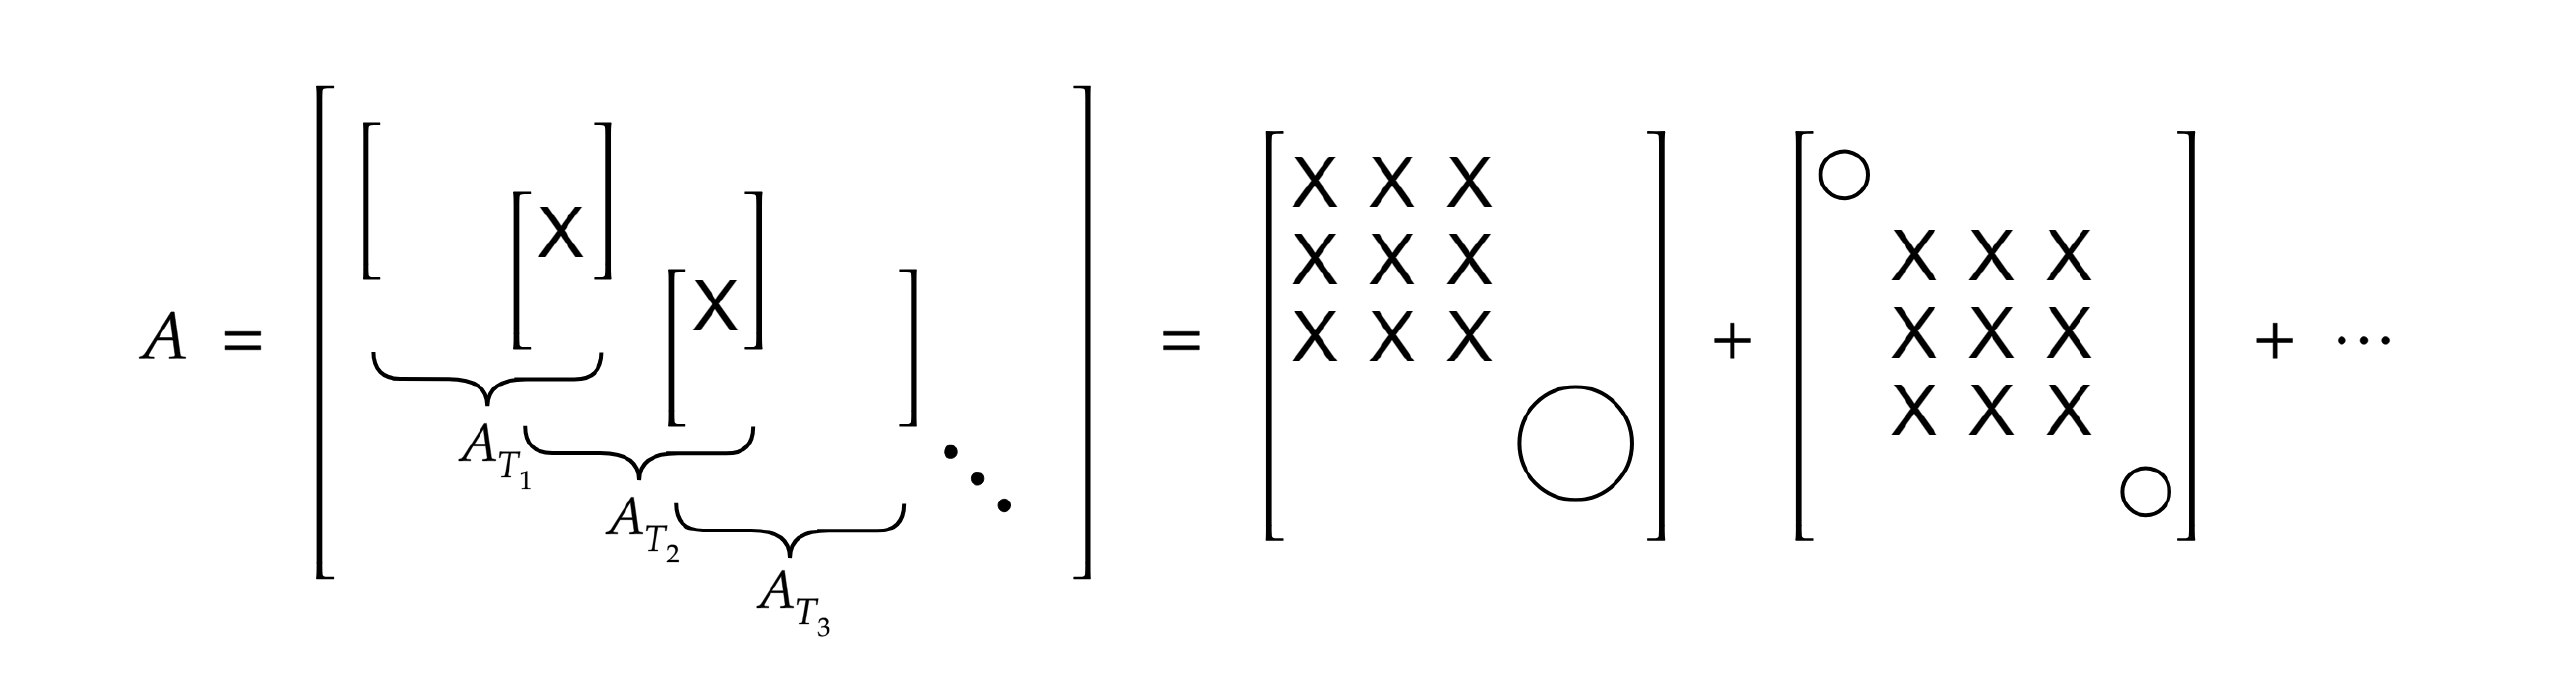
\includegraphics[width=\textwidth]{pics/chapter0/weird_matrix_equation.png}
	\end{center}
	\caption{Example of the global matrix}
	\label{fig:globalmatrixequation}
\end{figure}
\end{example}

In the following $V_{h}$ space of linear finite elements, i.e. $\overline{\P}= \overline{\P}_{1}$ and $T \in\mathcal{T}_{h}$ is a triangle in 2D:

\begin{lemma}
\label{thm:stiffnessmatrixlemma}
	The non-zero entries of the stiffness matrix $A$, $a_{i,j}$, on a triangular grid are given by
	\[
		a_{i,j} = -\frac{1}{2}(\text{cot}(\alpha_{i,j}) + \text{cot}(\beta_{i,j})) \quad\text{ and }\quad a_{i,i} = -\sum_{x_{j}\in N(x_{i})}^{}{a_{j,i}}
	.\] 
	with $N(x_{i})=\left\{ x_{j} \in \Omega _{h} : \left[ x_{i},x_{j}\right] \text{ is an edge in the grid}   \right\} $ and $\alpha_{i,j}$, $\beta_{i,j}$ denote angles opposite to the edge $e=[x_{i}, x_{j}]$ in the triangles adjacent to $e$

	\begin{figure}[H]
		\begin{center}
			

\tikzset{every picture/.style={line width=0.75pt}} %set default line width to 0.75pt        

\begin{tikzpicture}[x=0.75pt,y=0.75pt,yscale=-1,xscale=1]
%uncomment if require: \path (0,228.8571319580078); %set diagram left start at 0, and has height of 228.8571319580078

%Shape: Polygon [id:dp28921690697699165] 
\draw   (376.49,171.02) -- (257.3,215.26) -- (179.21,116.04) -- (250.14,10.49) -- (372.07,44.47) -- cycle ;
%Straight Lines [id:da4863938504467684] 
\draw    (372.07,44.47) -- (287.04,111.46) ;


%Straight Lines [id:da8762891187042963] 
\draw    (250.14,10.49) -- (287.04,111.46) ;


%Straight Lines [id:da2899192967452764] 
\draw    (179.21,116.05) -- (287.04,111.46) ;


%Straight Lines [id:da5127826797077264] 
\draw    (287.04,111.46) -- (257.3,215.26) ;


%Straight Lines [id:da15103321035376882] 
\draw    (376.5,171.02) -- (287.04,111.46) ;



%Shape: Circle [id:dp30610607134488066] 
\draw  [fill={rgb, 255:red, 0; green, 0; blue, 0 }  ,fill opacity=1 ] (284.79,111.46) .. controls (284.79,110.21) and (285.8,109.21) .. (287.04,109.21) .. controls (288.28,109.21) and (289.29,110.21) .. (289.29,111.46) .. controls (289.29,112.7) and (288.28,113.71) .. (287.04,113.71) .. controls (285.8,113.71) and (284.79,112.7) .. (284.79,111.46) -- cycle ;
%Shape: Circle [id:dp8033969897579307] 
\draw  [fill={rgb, 255:red, 0; green, 0; blue, 0 }  ,fill opacity=1 ] (374.24,171.02) .. controls (374.24,169.78) and (375.25,168.77) .. (376.49,168.77) .. controls (377.74,168.77) and (378.74,169.78) .. (378.74,171.02) .. controls (378.74,172.27) and (377.74,173.27) .. (376.49,173.27) .. controls (375.25,173.27) and (374.24,172.27) .. (374.24,171.02) -- cycle ;


%Shape: Arc [id:dp1378293688381258] 
\draw  [draw opacity=0] (268,177.95) .. controls (279.11,176.85) and (289.41,182.14) .. (292.81,191.57) .. controls (294.02,194.92) and (294.23,198.43) .. (293.57,201.84) -- (268.11,200.48) -- cycle ; \draw   (268,177.95) .. controls (279.11,176.85) and (289.41,182.14) .. (292.81,191.57) .. controls (294.02,194.92) and (294.23,198.43) .. (293.57,201.84) ;

%Shape: Arc [id:dp07595706892444554] 
\draw  [draw opacity=0] (372.99,82.51) .. controls (365.06,83.33) and (357.01,81.23) .. (350.56,75.99) .. controls (347.42,73.44) and (344.94,70.37) .. (343.12,66.98) -- (371.82,49.83) -- cycle ; \draw   (372.99,82.51) .. controls (365.06,83.33) and (357.01,81.23) .. (350.56,75.99) .. controls (347.42,73.44) and (344.94,70.37) .. (343.12,66.98) ;


% Text Node
\draw (291,97) node   {$i$};
% Text Node
\draw (388,170) node   {$j$};
% Text Node
\draw (277,194) node   {$\alpha _{ij}$};
% Text Node
\draw (363,67) node   {$\beta _{ij}$};
% Text Node
\draw (322,144) node   {$e$};
% Text Node
\draw (435,108) node   {$e\ =[ x_{i} ,x_{j}]$};


\end{tikzpicture}

		\end{center}
		\caption{Sketch of the involved part of the grid}
		\label{fig:pentagonrelations}
	\end{figure}
	

	\begin{itemize}
	\item Note: on boundary edges one side of the edge contributes to $a_{i,j}$
	\item Note: This form of stiffness matrix (Laplacian) is called \underline{Cotan-Laplacian} and can be derived by purely geometric arguments
	\item Note: The formula holds also for surface grids with $\text{dim}(\Omega _{h}) \neq \text{dim}(X)$
\end{itemize}

\end{lemma}

\begin{proof}
\label{thm:stiffnessmatrixlemmaproof}
\begin{enumerate}[label=\arabic{enumi})]
	\item The aspect ratio of a triangle can be expressed as the sum of $\cot$-s of the interior angles at its base.
		\[
		\frac{W}{h} = \cot \alpha + \cot \beta
		.\] 
		since
		\[
			\cot \alpha = \frac{W_{1}}{h},\quad \cot \beta = \frac{W_2}{h}
		.\] 
		\[
		\implies \frac{W_1}{h} + \frac{W_2}{h} = \frac{W}{h}
		.\] 
		\begin{figure}[H]
			\begin{center}
				

\tikzset{every picture/.style={line width=0.75pt}} %set default line width to 0.75pt        

\begin{tikzpicture}[x=0.75pt,y=0.75pt,yscale=-1,xscale=1]
%uncomment if require: \path (0,190.00892639160156); %set diagram left start at 0, and has height of 190.00892639160156

%Shape: Triangle [id:dp6112526830585387] 
\draw   (262.89,20.01) -- (464,130.01) -- (186,130.01) -- cycle ;
%Straight Lines [id:da511961550435736] 
\draw  [dash pattern={on 4.5pt off 4.5pt}]  (262.89,20.01) -- (263,81.01) ;


%Shape: Right Angle [id:dp8328437648465061] 
\draw  [dash pattern={on 4.5pt off 4.5pt}] (263,81.01) -- (262.99,130.01) -- (192.99,129.99) ;
%Shape: Arc [id:dp2718572053483814] 
\draw  [draw opacity=0] (409.25,130.01) .. controls (409.25,130.01) and (409.25,130.01) .. (409.25,130.01) .. controls (409.25,120.63) and (411.84,111.83) .. (416.38,104.22) -- (464,130.01) -- cycle ; \draw   (409.25,130.01) .. controls (409.25,130.01) and (409.25,130.01) .. (409.25,130.01) .. controls (409.25,120.63) and (411.84,111.83) .. (416.38,104.22) ;
%Shape: Arc [id:dp1192225319580984] 
\draw  [draw opacity=0] (203.03,105.31) .. controls (209.41,109.71) and (214.09,116.56) .. (215.54,124.79) .. controls (215.89,126.75) and (216.04,128.69) .. (216,130.6) -- (186,130.01) -- cycle ; \draw   (203.03,105.31) .. controls (209.41,109.71) and (214.09,116.56) .. (215.54,124.79) .. controls (215.89,126.75) and (216.04,128.69) .. (216,130.6) ;
%Shape: Brace [id:dp9341060012933176] 
\draw   (173,20.51) .. controls (168.33,20.51) and (166,22.84) .. (166,27.51) -- (166,65.26) .. controls (166,71.93) and (163.67,75.26) .. (159,75.26) .. controls (163.67,75.26) and (166,78.59) .. (166,85.26)(166,82.26) -- (166,123.01) .. controls (166,127.68) and (168.33,130.01) .. (173,130.01) ;
%Shape: Brace [id:dp0693567410987852] 
\draw   (184,149) .. controls (184,153.67) and (186.33,156) .. (191,156) -- (313.5,156) .. controls (320.17,156) and (323.5,158.33) .. (323.5,163) .. controls (323.5,158.33) and (326.83,156) .. (333.5,156)(330.5,156) -- (456,156) .. controls (460.67,156) and (463,153.67) .. (463,149) ;

%Shape: Arc [id:dp16382510809922857] 
\draw  [draw opacity=0] (263,110.75) .. controls (269.48,111.05) and (275.77,114.8) .. (279.23,121.14) .. controls (280.78,123.98) and (281.59,127.02) .. (281.71,130.01) -- (262.99,130.01) -- cycle ; \draw   (263,110.75) .. controls (269.48,111.05) and (275.77,114.8) .. (279.23,121.14) .. controls (280.78,123.98) and (281.59,127.02) .. (281.71,130.01) ;


% Text Node
\draw (215,68) node   {$b$};
% Text Node
\draw (368,61) node   {$a$};
% Text Node
\draw (423,120) node   {$\beta $};
% Text Node
\draw (203,120) node   {$\alpha $};
% Text Node
\draw (148.5,73) node   {$h$};
% Text Node
\draw (323,170) node   {$w$};
% Text Node
\draw (228,142) node   {$w_{1}$};
% Text Node
\draw (350,142) node   {$w_{2}$};
% Text Node
\draw (271,122) node   {$.$};


\end{tikzpicture}

			\end{center}
			\caption{Sketch of the used properties}
			\label{fig:triangleexplained}
		\end{figure}
	\item Let $\vec{e}$ be the edge vector along the base of the triangle $T$. The gradient of the hat-function $\phi$ associated with the opposite vertex $v$ is given by
		\[
		\nabla \phi = \frac{1}{2\abs{T} }\vec{e}^{\bot}
		,\] 
		where $\vec{e}^{\bot}$ is the vector $\vec{e}$ rotated by a quarter turn in counter-clockwise direction and $\abs{T} $ is the area of $T$.
	\item Using everything we get 
		\[
			\int_{T}\nabla \phi \nabla \phi \d x = \frac{1}{2}(\cot \alpha + \cot \beta)
		.\] 
	\item For $\phi _{i}, \phi _{j}$ associated with vertices $x_{i}, x_{j}$ on the same element $T$, we have
		\[
		\int_{T}\nabla  \phi _{i} \nabla \phi _{j} \d x = - \frac{1}{2}\cot \theta
		,\] 
		with $\theta$ opposite to edge $[x_{i}, x_{j}]$
		\begin{figure}[ht!]
			\begin{center}
				

\tikzset{every picture/.style={line width=0.75pt}} %set default line width to 0.75pt        

\begin{tikzpicture}[x=0.75pt,y=0.75pt,yscale=-1,xscale=1]
%uncomment if require: \path (0,129.99998474121094); %set diagram left start at 0, and has height of 129.99998474121094

%Shape: Triangle [id:dp34052386087480513] 
\draw   (331,21) -- (396.5,101) -- (265.5,101) -- cycle ;
%Shape: Arc [id:dp043023834573566955] 
\draw  [draw opacity=0] (353.04,47.67) .. controls (346.89,52.54) and (339.26,55.43) .. (331,55.43) .. controls (322.98,55.43) and (315.56,52.71) .. (309.5,48.09) -- (331,16) -- cycle ; \draw   (353.04,47.67) .. controls (346.89,52.54) and (339.26,55.43) .. (331,55.43) .. controls (322.98,55.43) and (315.56,52.71) .. (309.5,48.09) ;


% Text Node
\draw (331,110) node   {$e$};
% Text Node
\draw (262,110) node   {$x_{i}$};
% Text Node
\draw (404,110) node   {$x_{j}$};
% Text Node
\draw (331,41) node   {$\theta $};


\end{tikzpicture}

			\end{center}
			\caption{Sketch of the location of $\theta$}
			\label{fig:thetasketch}
		\end{figure}
		
\end{enumerate}
\end{proof}

\begin{remark}
\label{thm:stiffnessmatrixlemmaremark}
	We get the matrix vector product $A\cdot u = y$
	\begin{align*}
		y_{i} &= \sum_{j=1}^{n}{a_{i,j}u_{j}}\\
              &= \sum_{x_{j}\in N(x_{i})}^{}\underbrace{{\frac{1}{2}(\cot \alpha_{i,j}+ \cot \beta_{i,j})}}_{w_{i,j}}(u_{j}-u_{i}) \\
			  &= \sum_{x_{j}\in N(x_{i})}^{}{w_{i,j}(u_{j}- u_{i})}
	\end{align*}
\end{remark}

\begin{definition}
\label{thm:locallydelaunay}
	An edge $e$ of a triangulation $\mathcal{T}_{h}$ of $\Omega _{h}$ is \underline{locally Delaunay} if the sum of the angles opposite to $e$ in the adjacent triangles do not exceed $\pi $, i.e.
	\[
      e = [x_{i}, x_{j}] \qquad \alpha_{i,j} + \beta_{i,j}\overset{!}{\leq} \pi 
	.\] 
\end{definition}

\begin{definition}
\label{thm:delaunay}
	A triangulation is called \underline{Delaunay} if all interior edges are locally Delaunay.
\end{definition}

\begin{lemma}
\label{thm:delaunaylemma}
	For a Delaunay triangulation, the weights $w_{i,j}$ are non-negative and $A$ is a Z-matrix, i.e. $a_{i,j} \leq 0 \quad \forall i \neq j$
\end{lemma}

\begin{proof}
\label{thm:delaunaylemmaproof}
	\[
		\cot \alpha + \cot \beta = \frac{\sin(\alpha+\beta)}{\sin \alpha \sin \beta} \geq 0
	,\] 	
	if $\alpha + \beta \leq \pi $ and $\alpha,\beta \geq 0 $
\end{proof}

\underline{Summary}:
$A=(a(\phi _{i}, \phi _{j}))_{i,j}$ is (in a linear Lagrange triangulation setting)
\begin{itemize}
	\item symmetric
	\item sparse
	\item pos. definite
	\item Z-matrix if Delaunay
	\item $\abs{a_{i,i}} \geq \sum_{j}^{}{\abs{a_{i,j}} }$ + Delaunay for inner nodes
	\item irreducible
	\item $\text{diag}(A) \geq 0$
	\item number of non-zeros per row i : $\# \left\{ \text{ edges incident to node i } \right\} + 1$
\end{itemize}

\subsection{Finite-Element Refinement}
\label{sec:Finite-Element Refinement}

Consider two nested finite-element spaces.
\[
V_{H} \subset V_{h} \text{ on triangulations } \mathcal{T}_{H} \text{ and } \mathcal{T}_{h}
.\] 
respectively with 
\[
T = \bigcup_{j=1}^{m}t_{j} \text{ for all  } T \in \mathcal{T}_{H} \text{ with some } t_{j} \in \mathcal{T}_{h}
.\] 

\begin{exam}
\label{thm:refinementexamples}

\begin{itemize}
	\item bisection refinement
		% TODO : Bild 1
	\item red refinement
		% TODO : Bild 2
\end{itemize}
\end{exam}
We want to define a interpolation (prolongation) operator for the basis functions $\left\{ \phi _{i}^{H} \right\}_{i=1}^{K}$ of $V_{H}$ and $\left\{ \phi _{j}^{h} \right\} _{j=1}^{k}$ of $V_{h}$
\[
P_{H}^{h} \colon V_{H} \rightarrow V_{h}
.\] 
Since $V_{H} \subset V_{h}$ nested, the interpolation can be written as 
\[
P_{H}^{h}\phi _{j}^{H} = \sum_{i=1}^{k}{P_{i,j}\phi _{i}^{h}}
\] 
with $P = (P_{i,j})_{\substack{i=1, \ldots, k \\ j=1, \ldots, K}}$

Let $u^{H}=(u_{1}^{H}, \ldots , u_{K}^{H})$ and $u^{h}=(u_{1}^{h}, \ldots , u_{k}^{h})$ be the coefficient vectors of $u_{H} \in V_{H}$ and $u_{h} \in V_{h}$ respectively with respect to their basis $\left\{ \phi _{j}^{H} \right\} $ and $\left\{ \phi _{i}^{h} \right\} $.

Using the matrix $P$ from above, we conclude
\begin{align*}
	P_{H}^{h}u_{H} &= \sum_{j=1}^{K}{u_{i}^{H}P_{H}^{h}\phi _{i}^{H}} \\
				   &=\sum_{j=1}^{K}{u_{i}^{H}\sum_{i=1}^{k}{P_{i,j}\phi _{i}^{h}}} \\
				   &= \sum_{i=1}^{k}{(Pu^{H})_{i}\phi _{i}^{h}}
\end{align*}
and thus $u^{h} = Pu^{H}$ (where $u^{h}$ represents the coefficients on $\mathcal{T}_{h}$ respectively the coarse grid function $u_{H}$)

For model Lagrange FE, with Lagrange nodes $\left\{ x_{i} \right\} $, we have the relation
\[
	\phi _{i}(x_{j}) = \delta_{ij} \qquad \forall \phi _{i} \text{ in basis of } V_{h}
.\] 
Let $\left\{ x_{i}^{H} \right\} $ be the Lagrange nodes on $\mathcal{T}_{H}$ and $\left\{ x_{i}^{h} \right\} $ be the Lagrange nodes on $\mathcal{T}_{h}$.

The matrix $P$ is given by
\[
	P_{i,j} = \phi _{j}^{H}(x_{i}^{h}) \qquad 
	\begin{array}{l}
	i=1, \ldots, k \\
	j=1, \ldots, K
	\end{array}
.\] 
Galerkin relation between stiffness matrix $A_{h}$ and $A_{H}$.
\begin{align*}
	A_{H} &= (a_{H}(\phi _{r}^{H}, \phi _{s}^{H}))_{r,s}\\
	A_{h} &= (a_{h}(\phi _{r}^{h}, \phi _{s}^{h}))_{r,s}\\
\end{align*}
\begin{align*}
	a_{H}(\phi _{r}^{H}, \phi _{s}^{H}) &= a_{h}(P_{H}^{h}\phi _{r}^{H}, P_{H}^{h}\phi _{s}^{H}) \\
										&= a_{h}(\sum_{i=1}^{k}{P_{i,r}\phi _{i}^{h}}, \sum_{j=1}^{k}{P_{j,s}\phi _{j}^{h}}) \\
										&= \sum_{i,j=1}^{k}{P_{i,r}a_{h}(a_{i}^{h}, a_{j}^{h}) P_{j,s}}
\end{align*}
So
\[
	A_{H} = (P_{H}^{h})^{T}A_{h}P_{H}^{h}
\]
and thus we define the restriction operator as
\[
	R_{h}^{H} = (P_{H}^{h})^{T}
.\] 

	\section{Lineare Optimierung}
ganzzahlige Lineare Programme:
\begin{equation*}
	\min_{x} c^Tx \text{ subject to } \quad Ax = b, x \geq 0, x \in \Z^n
\end{equation*}
Zusätzliche obere Schranken für die Variablen sind auch möglich.
Beispielsweise wäre durch $0 \leq x \leq 1$, $x \in \Z^n$ ein binäres Problem gegeben.
\subsection{Optimalitätsbedingungen für kontinuierliche LPs}
\begin{itemize}
	\item LP in Normalform
		\begin{equation}\label{nf}
			\min_{x} c^Tx \text{ subject to } Ax = b, x\geq 0\tag{P}
		\end{equation}
	\item Die zulässige Menge ist ein Polyeder:
		\begin{equation*}
			P = \{ x | Ax = b ,x \geq 0 \}
		\end{equation*}
  \item Problem konvex (d.\,h\ Zielfunktion und zulässige Menge sind konvex) $\to$	lokale Minima = globale Minima
  \item Das dazu \underline{duale Problem} ist gegeben durch
		\begin{equation*}\label{dual_cont}
			\max_{y}b^Ty \text{ subject to } A^Ty \leq c, y \in \R^n \tag{D}
		\end{equation*}
\end{itemize}
\begin{lemma}[Schwache Dualität] \label{thm:schwache_dualitat}
		Es gilt für alle $x$ zulässig für \eqref{nf} und alle $y$ zulässig für \eqref{dual_cont}:
		\begin{equation*}
			c^Tx \geq b^Ty
		\end{equation*}
		Bei Gleichheit gilt außerdem: $x$ löst \eqref{nf}, $y$ löst \eqref{dual_cont}.
\end{lemma} % end lemma Schwache Dualität
\begin{lemma}[Starke Dualität] \label{thm:starke_dualitat}
  Es sind äquivalent
  \begin{enumerate}
    \item \eqref{nf} hat eine Lösung $x^*$.
    \item \eqref{dual_cont} hat eine Lösung $y^*$.
    \item $(x^*,y^*)$ lösen das \underline{KKT-System}
      \begin{align*}
        Ax^* &= b , \ x^* \geq 0 & \text{(primale Zulässigkeit)}\\
        A^{T} y^* &\leq c & \text{(duale Zulässigkeit)}\\
        \forall i = 1,\dots , n: x_{i}&= 0 \text{ oder } \left(A^{T}y^*  \right)_{i} = c_{i} & \text{ (Komplementaritätsbedingungen)}
      \end{align*}
      Dann gilt auch, dass die \underline{Dualitätslücke} gleich $0$ ist:
      \begin{equation*}
        b^{T}\underbrace{y^* = (\underbrace{x^*}_{\geq 0})^{T}}_{\text{primal Zul.}} \underbrace{\underbrace{A^{T} y^*}_{\leq c }}_{\text{dual Z.}} \stackrel{\text{Kompbed.}}= \left(x^*\right)^{T} c
      \end{equation*}
    \end{enumerate}
\end{lemma} % end lemma Starke Dualität
\paragraph{Lösungsansätze für lineare Programme}
\begin{itemize}
  \item Innere-Punkte-Verfahren. (polynomielle Laufzeit)
  \item Ellipsoid-Verfahren. (polynomielle Laufzeit)
  \item Symplex-Verfahren (theoretisch exponentielle Laufzeit, aber in der Praxis gut)
\end{itemize}
\paragraph{Ecken und Lösungen}
\begin{itemize}
  \item $\hat{x}$ ist Ecke von $P$ $\iff$ $ \hat{x}$ kann nicht als echte Konvexkombination von Punkten aus $P$ geschrieben werden
		$\iff$ Sei
		\begin{equation*}
			I = \{i = 1 ,\dots, n | \hat{x}_{i} \geq 0 \} = \supp(\hat{x})
		\end{equation*}
		Dann gilt $\rang(A_{\cdot,I})=|I|$.
	\item Hat das LP \eqref{nf} eine Lösung, so gibt es auch eine Ecklösung.
	\item Es gibt nur endlich viele Ecken.
	\item Idee des Simplex-Verfahrens: Ecken von $P$ in sinnvoller Reihenfolge absuchen.\\
		\underline{Annahme:} $A \in \R^{m \times n }$ hat \underline{vollen Zeilenrang} $m$. \\
		Sei $\hat{x}$ eine Ecke von $P$ und $I = \{i \mid \hat{x}_{i}>0\}$ \\
		$\implies$ rang($A_{\cdot,I}   )= |I| \leq m$ \\
    $\implies$ Es gibt $B \subseteq \{1,\dots,n\}$ mit $I \subseteq B, |B| = m $ und $A_{B}:= A_{\cdot,B}$ ist regulär. (Finde $B$ durch Basisergänzung, da $A$ $m$ linear unabhängige Spalten hat.)
	\item Basen\\
		Sei $B \subset \{1,\dots,n\}$ mit $|B|=m$ und $N = \{1,\dots,n\}\setminus B$
    \begin{itemize}[label=$\to$] % warum eigentlich ein Pfeil?
      \item $B$ heißt \underline{Basis}, falls $A_{B}$ regulär.
      \item $B$ heißt \underline{primal zulässige Basis}, falls
        \begin{equation*}
          x_{B}=A_{B}^{-1}b \geq 0
        \end{equation*} $\implies$ Mit $x_{N} = 0$ ist $(x_{B},x_{N})$ zulässig für \eqref{nf} und eine Ecke von $P$.
      \item $B$ heißt \underline{dual zulässige Basis}, falls
        \begin{equation*}
          A_{N}^TA_{B}^{-T}c_{b} \leq c_{N} \implies y \text{ ist zulässig für \eqref{dual_cont}}
        \end{equation*}
      \item $\left(x_{B},x_{N} \right)$ mit $x_{B} = A^{-1}_{B},\ x_{N}= 0$ heißt \underline{Basislösung}. Ist $x_{B} > 0 $ so heißt die Basislösung \underline{nichtdegeneriert}.
        (Im degenerierten Fall kann $B$ unterbestimmt sein, man bleibt u.\,U.\ in der gleichen Ecke.)
    \end{itemize}
\end{itemize}
%
\subsection{Wiederholung Simplex-Verfahren}
Annahme: $A \in R^{m \times n}$ hat Rang $m$. (Ansonsten können so lange linear von den anderen Zeilen abhängige Zeilen gelöscht werden, bis $A$ vollen Zeilenrang $m$ hat.)

Sei $B$ eine primal zulässige Basis mit Basislösung
\begin{align*}
	\hat{x}_{N}&=0,\\
	\hat{x}_{B}&= A_{B}^{-1}b
\end{align*}
Für alle $x \in P$ gilt:
\begin{align*}
	Ax&=
	\begin{pmatrix}
		A_{B} & A_{N}
	\end{pmatrix}
	\begin{pmatrix}
		x_{B} \\ x_{N}
	\end{pmatrix}
	\\
	  & A_{B}x_{B} + A_{N}x_{N}= b
\end{align*}
$\implies x_{B} = A_{B}^{-1}b - A_{B}^{-1}A_{N}x_{N} \to$ Zielfunktion vereinfachen
\begin{align*}
	c^Tx&= c_{B}^Tx_{B} + c_{N}^Tx_{N} = c_{B}^T \underbrace{A_{B}^{-1}b}_{= \hat{x}_{B}} - c_{B}^TA_{B}^{-1}A_{N}x_{N} + c_{N}^Tx_{N}\\
		&= c^{T}_{B} \hat{x}_{B} +( \underbrace{ c_{N} - A_{N}^{T} \underbrace{A_{B}^{-T}c_{B}}_{=y} }_{=: z_{N}, \text{ reduzierte Kosten}} )^{T} x_{N}
\end{align*}

\begin{itemize}
	\item Gilt $z_{N} \geq 0$: $\hat{x}$ löst LP (mit dualer Variable $y$)
	\item Andernfalls: Wähle $j\in \N$ mit $z_{j}<0$.

		Frage: Wie groß kann $x_{j}$ gewählt werden, ohne $P$ zu verlassen?

		Wir wählen das neue $x_{N}$ als $\gamma e_{j}$ mit zu bestimmenden $\gamma$.
		\begin{itemize}
      \item[$\implies$] neues $x_{B}
        = \hat{x}_{B} - A_{B}^{-1}A_{N}\gamma e_{j}
        = \hat{x}_{B} - \gamma \underbrace{A_{B}^{-1}A_{\cdot,j}}_{=: w}
        \overset{!}{\geq} 0$
			\item Wähle $\gamma = \min \left\{ \frac{\hat{x}_{i}}{w_{i}} \mid w_{i} > 0 \right\}$.
      \item Wenn $\gamma = + \infty$, so ist \eqref{nf} unbeschränkt.
			\item Andernfalls wähle $i \in B$ mit $\gamma = \frac{\hat{x}_{i}}{w_{i}}$
		\end{itemize}
  \item Dann ist die neue Ecke $x_B^+$
		\begin{align*}
			\hat{x}_{B}-\gamma_{w}&= x_{B}^+\\
			x_{j}^+& = \gamma\\
			x_{k}^+ &= 0 \quad \text{ für alle anderen } k\\
			B^+ &= (B \setminus \{i\})\cup \{j\}\\
			N^+ &= (N \setminus \{j\})\cup \{i\}
			% B& = \{1,3,5\} \\
			% B& = (3,1,5)
		\end{align*}
    Pro Iteration müssen zwei Gleichungssysteme gelöst werden. Das ist sehr teuer. Da sich immer nur $1$ Spalte ändert, kann dies allerdings stark vereinfacht werden durch ein Update der LR-Zerlegung. Das geht, indem in der Implementierung die Elemente von $B$, $B^+$ eine Reihenfolge haben und man ersetzt immer $i$ an seiner Stelle durch $j$.
\end{itemize}
\paragraph{Startbasis}
Gesucht als Startbasis ist eine primal zulässige Basis für
\begin{equation*}
	\min_{x} c^Tx \text{ subject to } Ax = b , x \geq 0
\end{equation*}
Dafür gibt es die Simplex-Phase 1: Löse das Hilfsproblem
\begin{align*}
	\min_{x,s} \sum_{i=1}^{m} s_{i} \text{ subject to }
	\begin{pmatrix}
		A& I
	\end{pmatrix}
	\begin{pmatrix}
		x \\ s
	\end{pmatrix}
	, (x,s)& \geq 0
\end{align*}
Gilt in einer Lösung ($x^0$), dass $s^* =0$, so ist das $x^*$ zulässig für \eqref{nf} und die Basis des Hilfsproblems \enquote{ist} eine primal zulässige Basis für \eqref{nf}.

Eine primal zulässige Startbasis für das Hilfsproblem ist (trivialerweise) gegeben durch
\begin{equation*}
	x = 0, s = b \geq 0, \text{ Basismatrix } I
\end{equation*}
Tableau-Methode für %TODO: was sollen uns diese Zeilen sagen?
\begin{equation*}
	\min_{x}c^Tx \text{ subject to } Ax \leq b , x \geq 0
\end{equation*}
\section{Duales Simplex-Verfahren}
\begin{align}
  \text{primales LP} && \min_{x}c^{T} x \text{ subject to }Ax = b, x \geq 0 \tag{P} \label{primalLP} \\
  \text{duales LP} && \max_{y}b^{T} y \text{ subject to }A^{T} y \leq c, y \geq 0 \tag{D}\label{dualLP}
\end{align}
Wir nehmen wieder an, dass $A \in \R^{m \times n}$ Rang $m$ hat.

Für eine Basis $B$ ist wie bisher $x_{B}= A^{-1}_{B}b, x_{N}=0$.

\underline{Idee:} Wende Simplex-Verfahren auf \eqref{dualLP} an.
Dafür führe \eqref{dualLP} in die duale Normalform:
\begin{equation}\label{dualnf}
	\max_{y} b^{T} y \text{ subject to }
	\begin{pmatrix}
		A^{T} & I
	\end{pmatrix}
	\begin{pmatrix}
	y\\z
	\end{pmatrix}
	= c, \quad z \geq 0, \quad y \in \R^m \tag{D'}
\end{equation}
Eine Basis von \eqref{dualnf}: $n \{ \klammern[\Big]{ \underbrace{A^T}_m \underbrace I_n} =: D
% \begin{pmatrix}
% 	\underbrace{A^{T}}_{m} \underbrace{I}_{n}
% \end{pmatrix}
\in R^{n \times(m +n)}$
sei $H \subset \{1,\dots ,n+m \}$ mit $|H|=n$ und $D_{\cdot,H}\in \R^{n \times n}$ regulär.
\begin{theorem}
	Entweder \eqref{dualLP} ist unzulässig oder unbeschränkt oder es gibt eine optimale Basislösung $(y^*,z^*)$ so dass die zugehörige basis von der Form ist:
	\begin{equation*}
    H_{\text{opt}}=\underbrace{ \{1,..,m \}}_{\text{ganzes $A$ in Basismatrix}}\cup \, (N+\underbrace{m}_{\text{offset}})
	\end{equation*}
	mit $N \subset \{1,\dots ,n \}, |N|= n-m$ ($N$ zeigt an, welche Spalten von $I$ gebraucht werden)
	$\implies$ Basen für \eqref{dualLP} werden i.A. durch $N$ beschrieben, nicht durch $H$.
\end{theorem}
Die Dualität sagt uns, dass die Indices der Nullvariablen in \eqref{nf} gerade die Elemente von $N$ sind, nämlich die Nicht-Null-Schlupfvariablen.

Welche Basis $H$ bzw. $N$ liefert eine zulässige Basislösung für \eqref{dualLP}?
% irgendwas kompiliert hier nicht
\begin{align*}
  \begin{pmatrix}
    A^{T}  & I
  \end{pmatrix}
  \begin{pmatrix}
    y\\z
  \end{pmatrix}
  &=c, \quad z \geq 0\\
  \iff \begin{pmatrix}
      A_N^T & I_N & 0 \\
      A_B^T & 0 & I \\
    \end{pmatrix}
    \begin{pmatrix}
      y \\ z_N \\ z_B
    \end{pmatrix}
    &= \begin{pmatrix}
    c_N \\ c_B
  \end{pmatrix}
  , \quad z \geq 0 \quad (\text{nach Zeilenumsortierung})\\
  \iff A_{B}^{T} y + z_{B} &= c_{B}, \quad z_{B} \geq 0\\
    A_{N}^{T} y + z_{N} &= c_{N}, \quad z_{N} \geq 0 \\
    \iff y &= A_{B}^{-T}(c_{B}-z_{B})\\
      z_{N}&= c_{N} - A_{N}^{T}y = c_{N}-A_{N}^{T} A_{B}^{-T}(c_{B}-z_{B}) ,\quad z_{B}\geq 0, z_{N} \geq 0
\end{align*}
Wenn $(y,z_{B},z_{N})$ eine Basislösung ist, so sind die Nichtbasisvariablen $z_{B} =0$.
Also
\begin{equation*}
	y = A_{B}^{-T}c_{B}, \quad z_{N}= c_{N}- A_{N}^{T} \underbrace{A_{B}^{-T}c_{B}}_{{=y}}\geq 0
\end{equation*}
\subsection{Duales Simplex-Verfahren}
Initialisierung: Dual zulässige Basis $B$, d.\,h.\ $B \subset \{1,\dots ,n \}$ mit $|B|=m$, $A_{B}$ regulär und $z_{B}=0$, $y=A_{B}^{-T}c_{B}$, $z_{N}= c_{N}-A_{N}^{T}y \geq 0$
\begin{enumerate}%[label = Schritt \arabic)]
	\item Bestimme zugehörige komplementäre duale Variable
		\begin{align*}
			x_{N}&=0 \quad (\to \text{komplementär zu }z_{N})\\
      x_{B}&= A_{B}^{-1} b\quad \left( \implies A \begin{pmatrix}x_{B} \\ x_{N}\end{pmatrix} =b\right)
		\end{align*}
	\item Gilt $x_{B} \geq 0 $: \textbf{Stop}.\\
    $(y,z_{B},z_{N}),(x_{B},x_{N})$ KKT-Punkt $\implies$ Lösung gefunden.\\
		Andernfalls wähle $ i \in B$ mit $x_{i}<0$ ($\to z_{i}>0$ verkleinert dualen Zielfunktionswert)
	\item Löse $A_{B}^{T} w = e_{i}$, $\alpha_{N} = -A_{N}^{T} w$
	\item Schrittweitenbestimmung:\\
    Gilt $\alpha_{N} \leq 0 $: \textbf{Stop}, \eqref{dualLP} ist unbeschränkt ($\to$ \eqref{nf} unzulässig).\\
		Andernfalls berechne $\gamma = \min \left\{ \frac{z_{i}}{\alpha_{i}} \mid j \in N , \alpha_{j} >0 \right\}$ und wähle $j \in N$ mit $\gamma = \frac{z_{j}}{\alpha_{j}}$
	\item Update:
		\begin{align*}
			z_{N}^+ &= z_{N} - \gamma \alpha_{N} \quad (\to z_{N} \geq 0, z_{j}^+ =0)\\
			z_{i}^+ &= \gamma\\
			y^+ &= y -\gamma w\\
			N^+ &= (N \backslash \{ j \}) \cup \{ i \}\\
			B^+ &= (B \backslash \{ i \}) \cup \{ j \}
		\end{align*}
\end{enumerate}

\subsection{(primales) Simplex-Verfahren für LPs mit Schranken}
Betrachte
\begin{equation*}
	\min_{x} c^{T} x \text{ subject to } Ax = b ,\quad l \leq x \leq u
\end{equation*}
mit $l \in \left(\R \cup \{ - \infty \} \right)^n$, $u \in \left(\R \cup \{ +\infty \} \right)^n $.

% Mit bis zu $4n$ Schlupfvariablen kann das System auf Normalform gebracht werden. Allerdings bedeutet das ein Vielfaches an Rechenaufwand. Daher suchen wir andere Wege.
%
\underline{Ziel:} möglichst nahe an die Form
\begin{equation*}
	\min_{x} c^{T} x \text{ subject to } Ax = b ,\quad x \geq 0
\end{equation*}
kommen.\\
\underline{mögliche Modifikationen:}
\begin{itemize}
	\item Schlupfvariablen + Variablensplit $x = x^+ -x^-, x^+,x^- \geq0 $ (Nachteil: erhöht die Anzahl der Variablen und linearen Gleichungen)
	\item Fall: $x_{i} \geq l_{i}$ mit $l_{i}\in \R$ : Substituiere $\hat{x}_{i} := x_{i}- l_{i}\geq 0$
	\item Fall: $x_{i} \leq u_{i}$ mit $u_{i}\in \R$ : Substituiere  $\hat{x}_{i} := u_{i}- x_{i}\geq 0$
	\item Fall: $l_{i} \leq x_{i} \leq u_{i}$ mit $l_{i},u_{i} \in \R$ : Substituiere $0 \leq \hat{x}_{i} := x_{i}- l_{i} \leq u_{i}-l_{i}$
	\item Fall $-\infty \leq x_{i} \leq \infty$ : Freie Variable: entweder Variablensplit $x_{i}= x_{i}^+ - x_{i}^-$ oder $x_{i}$ als freie Variable im Simplex-Verfahren berücksichtigen (wie $y$ im dualen Simplex)
\end{itemize}
Angenommen, es gibt keine freien Variablen $\implies$ oBdA LP der Form
\begin{equation*}
	\min_{x} c^{T} x \text{ subject to } Ax = b, \quad 0 \leq x \leq u
\end{equation*}
mit $u \in [0, + \infty]^n$.\nl
Bisher im primalen Simplex-Verfahren:\\
Basis $B$, Basisvariablen $x_{B}= A_{B}^{-1} b \geq 0$, Nichtbasisvariablen $x_{N}=0$ \\
\underline{Idee:} Teile die Nichtbasisvariablen in
\begin{align*}
	N_{l} &= \left\{ i \in N \ | \ x_{i} = 0  \right\} \implies x_{N_{l}}=0\\
	N_{u} &= \left\{ i \in N \ | \ x_{i} = u_{i}  \right\} \implies x_{N_{u}}=u_{N_{u}}
\end{align*}
Wie im Simplex-Verfahren:
\begin{align*}
	A_{B}x_{B} + A_{N_{l}}x_{N_{l}} + A_{N_{u}} x_{N_{u}} = b \implies x_{B} = A_{B}^{-1} (b - A_{N_{l}} x_{N_{l}} - A_{N_{l}}x_{N_{l}})\\
	c^{T} x = c_{B}^{T} x_{B} + c_{N_{l}}^{T} x_{N_{l}}+c_{N_{u}}^{T} x_{N_{u}} = c_{B}^{T} A_{B}^{-1} b + z_{N_{l}}^{T} x_{N_{l}} + z_{N_{u}}^{T} x_{N_{u}}
\end{align*}
Identifiziere $i \in N_{l}$ mit $z_{i} <0 $ oder $ i\in N_{u}$ mit $z_{i}> 0$.\\
Bei Schrittweiten beachten: $x_{B} = \gamma w \in [0,u_{B}]$ und
\begin{equation*}
	x_{i}^+ = \begin{cases}
	 \gamma \in [0,u_{i}]\\
	 u_{i}-\gamma
\end{cases}
\end{equation*}
Beim Basisupdate gibt es den neuen Fall $B^+ = B$, $i$ wechselt von $N_{l}$ nach $N_{u}$ oder umgekehrt.
\begin{beispiel}[Zuschnittsoptimierung]~\nl
  	\underline{Problemstellung} Eine vorgegebene Anzahl von Objekten soll möglichst materialsparend aus einem Grundstoff zugeschnitten werden.\\
  	\underline{konkretes Beispiel}: Eine Firma produziert Metallstangen mit Länge $100\,$cm. Werden kürzere Stangen bestellt muss die Firma $100\,$cm lange Stangen zerschneiden. Ziel der Firma ist es, die Bestellungen zu erfüllen und dafür möglichst wenige Stangen zerschneiden zu müssen.\\
  	Bestellung:
	\begin{table}[H]
		\centering
		\begin{tabular}{c|c}
			Länge in cm & Anzahl bestellt\\
      		\hline
      		$25$ & $80$ \\
      		$30$ & $75$ \\
      		$35$ & $105$ \\
  		\end{tabular}
	\end{table}
	\underline{Modellierung}
  \begin{enumerate}[label={Variante \arabic*.}]
    \item \label{item:Zuschnittsillymodel} Für jeden Stab $i$ beschreiben $x_{i1},x_{i2},x_{i3} \in \N_{0}$, wieviele Stäbe der Länge $25,30,35\,$cm daraus geschnitten werden sollen.
      \begin{align}
        \implies \forall i~ & 25x_{i1} + 30x_{i2} + 35x_{i3}\leq 100 \notag\\
                            &
        \begin{rcases}
          \sum\limits_{i}^{} x_{i1} \geq 80\\
          \sum\limits_{i}^{} x_{i2} \geq 75\\
          \sum\limits_{i}^{} x_{i3} \geq 105
        \end{rcases} \tag{$\Delta$}\label{model_cutting_1}
      \end{align}
      Zielfunktion: minimiere $K = \text{ Anzahl der Stäbe}$, wobei $i = 1,\dots ,K$.
      Um $K$ zu berechnen, nutze folgende Idee: Für jeden Stab $i$ führe eine Variable $y_{i} \in \left\{0,1 \right\}$ ein, die entscheidet, ob der Stab verwendet wird oder nicht.

      Die maximale Anzahl benötigter Stäbe ist $\leq 80 + 75 +105 = 260$.
      \begin{align*}
        \implies \min_{x,y}\sum_{i=1}^{260} y_{i} &\text{ subject to } x_{i1},x_{i2},x_{i3} \in \N_{0}, y_{i}\in \left\{0,1 \right\} , \eqref{model_cutting_1},\\
                                                  & \forall i = 1,\dots ,260 : 25x_{i1} + 30x_{i2} + 35x_{i3} \leq 100y_{i}
      \end{align*}
      \underline{Problem:} gigantisch viele Variablen und Restriktionen und Redundanz in der Darstellung. Das ist ein schlechtes Zeichen für das Modell, aber kein prinzipielles Problem für das Symplex-Verfahren. (Redundanz bedeutet in diesem Fall u.\,a., dass es sehr viele äquivalente Situationen gibt.)
    \item \label{item:Zuschnittbettermodel} Schnittmuster\\
     	Führe eine Variable $x_{i} \in \N_{0}$ ein für jedes Schnittmuster $i$, nach dem eine Stange zerschnitten werden kann:
      \begin{table}[H]
        \centering
        \begin{tabular}{c|c|c|c}
          Schnittmuster & \# $25\,$cm Stäbe & \# $30\,$cm Stäbe & \# $35\,$cm Stäbe\\
          \hline
          1 & 4 & 0 & 0\\
            & 3 & 0 & 0\\
          2 & 2 & 1 & 0\\
          3 & 2 & 0 & 1\\
          4 & 1 & 2 & 0\\
          5 & 1 & 1 & 1\\
          6 & 1 & 0 & 2\\
          7 & 0 & 3 & 0\\
          8 & 0 & 2 & 1\\
          9 & 0 & 1 & 2\\
        \end{tabular}
		\end{table}

    Optimierungsproblem:
    \begin{align*}
      \min_{x} \sum_{i=1}^{9} x_{i}& \text{ subject to } x \in \Z_{0}, x\geq 0
    \end{align*}
    \begin{align*}
      \text{mindestens } &80 \text{ Stäbe mit $25$\,cm}& 4x_{1} + 2x_{2} + 2x_{3} + x_{4} + x_{5} + x_{6} &\geq 80\\
                         &75\text{ Stäbe mit $30$\,cm}& x_{2} + 2x_{4} + x_{5} + 3x_{7} + 2x_{8} + x_{9} &\geq 75\\
                         &105\text{ Stäbe mit $35$\,cm}& x_{3} + x_{5} + 2x_{6} + x_{8} + 2x_{9} &\geq 105
    	\end{align*}
		In Matrixform $Hx \leq b$.

		Vorteil:
		\begin{itemize}
			\item Anzahl Restriktionen $=$ Anzahl verschiedener Stablängen
      \item Anzahl Variablen $=$ Anzahl (sinnvoller) Schnittmuster (wächst schnell, aber langsamer als \ref{item:Zuschnittsillymodel})
		\end{itemize}

 \end{enumerate}
 \underline{Lösung für \ref{item:Zuschnittbettermodel}}
\begin{enumerate}
	\item Statt des ganzzahligen LPs
		\begin{equation*}
			\min_{x} c^{T} x \text{ subject to } Mx \geq b, x \geq 0 , x \in \Z^{n}.
		\end{equation*}
		Löse das \underline{relaxierte LP}
	\begin{equation*}
		\min_{x} c^{T} x \text{ subject to } Hx \geq b, x \geq 0
	\end{equation*}
	\item Simplex-Verfahren für das relaxierte Problem:
		\begin{itemize}
			\item Wir brauhchen eine primal zulässige Startbasis:\\
			$\to$ Für jede Stablänge $l = 25,30,35$ verwende das \glqq Einheitsschnittmuster\grqq\ bei dem die maximal mögliche Anzahl $\lfloor\frac{100}{l}\rfloor$ von Stäben der Länge $l$ und keine anderen Stablängen geschnitten werden.


			Dann sind die zugehörigen Spalten in der Basismatrix linear unabhängige Vielfache von Einheitsvektoren.

		Die zugehörigen Basisvariablen sind:
		\begin{equation*}
			x_{l} = \frac{b_{l}}{\lfloor\frac{100}{l}\rfloor}
		\end{equation*}

		\item $H$ kann sehr viele Spalten haben.

			\underline{Idee:} Immer nur die Spalten von $H$ bestimmen, die man aktuell braucht.\\
			$\to$ Startbasis und zugehörige Basismatrix $A_{B} := \begin{pmatrix}
				H,&-I
			\end{pmatrix}_{B}
      $ wie oben bestimmen ($-I$ kommt von den Schlupfvariablen, die man braucht um aus $\geq$ ein $=$ zu machen).

			$\to$ zugehörige duale Variable:
			\begin{equation*}
				y = A_{B}^{-T}c_{B}
			\end{equation*}
			$\to $ reduzierte Kosten
			\begin{equation*}
				z_{N} = c_{N} - A_{N}^{T} y
			\end{equation*}
      Hierbei ist $c$ von der Form $c = (\underbrace{1 \, \ldots \, 1}_{x-\text{Teil}} \, \underbrace{0 \, \ldots \, 0}_{s- \text{Teil}})^T$.

      Für $j \in N$, die zu den Schlupfvariablen $s$ gehören, gilt
			\begin{equation*}
				z_{j} = c_{j} - A_{\cdot j}^{T} y = 0 + e_{j}^{T} y = y_{j}
			\end{equation*}
			($y_{j}$ ist bekannt). Für $j \in N$, die zu den Variablen $x$ gehören, gilt
			\begin{equation*}\label{dantzigRegel}
				e_{j} = c_{j} - A_{\cdot j}^{T} y = 1 - \underbrace{H_{\cdot j}^{T}}_{\text{unbekannt}} y \to \min \tag{Dantzig Regel}
			\end{equation*}
      Wir müssen also die \glqq beste\grqq{} Spalte $H_{\cdot j}$ als Lösung von
			\begin{equation*}
				\max_{h} y^{T} h \text{ subject to } 25h_{1} + 30 h_{2} + 35h_{3} \leq 100, h\geq 0 , h \in \Z^3
			\end{equation*}
      bestimmen. Damit erhalten wir ein Rucksackproblem mit Gewichten $=$ Stablängen und Werte $=$ duale Variable $y$. Dieses Rucksackproblem ist ganzzahlig, aber recht klein.
		\item Sei $x_{\alpha} \in \R^n$ eine Lösung des relaxierten Problems.
			\begin{enumerate}[label = \arabic*. Fall:]
				\item $x^* \in \Z^n \implies x^*$ löst auch das ganzzahlige LP.
				\item $x^* \not \in \Z^n$
          \begin{description}
            \item [Branch \& Bound Verfahren]
              $\implies$ zwei neue LPs
              \begin{align*}
                \min_{x} c^{T} &x \text{ subject to } Ax = b , x\geq 0 , x\leq \lfloor x_{i}^*\rfloor\\
                \max_{x} c^{T} &x \text{ subject to } Ax = b , x\geq 0 , x\geq \lceil x_{i}^*\rceil
              \end{align*}
              Für Branch \& Bound Verfahren muss man Techniken entwickeln um nicht den gesamten Baum an erstellten LPs durchsuchen zu müssen.
            \item [Schnittebenen-Verfahren]
              Füge neue Ungleichung
              \begin{equation*}
                a^{T} x \leq \beta
              \end{equation*}
              mit $a^{T} x \leq \beta$ für alle zulässigen Punkte $x \in \Z^n$ und $a^{T} x^* > \beta $ zu den Restriktionen hinzu.
              Im Idealfall werden dabei alle Ecken des zulässigen Polyeders ganzzahlig damit das Simplex-Verfahren eine ganzzahlige Lösung findet.
            \item [(Runden)] Ergibt in der Regel eine gute, aber keine optimale Lösung. Man muss aufpassen, zulässig zu bleiben. Beim Zuschnittsproblem kann man immer aufrunden.
          \end{description}
			\end{enumerate}
		\end{itemize}
\end{enumerate}
\end{beispiel}
\subsection{Polyeder}
\begin{definition}
	\begin{itemize}
    \item Eine Menge $P\subset \R^n$ heißt Polyeder, wenn man sie durch endlich viele lineare Ungleichung beschreiben kann.
      (Die Endlichkeitseinschränkung ist wichtig um Polyeder von beliebigen konvexen Mengen zu unterscheiden, denn jede konvexe Menge lässt sich durch (unendlich) viele lineare Ungleichungen beschreiben.)
		\item \underline{natürliche Form} eines Polyeders:
			\begin{align*}
				P(A,b) &= \left\{ x \in \R^n \ \middle| \ a^{T}_{i} x \leq b_{i} \ \forall i =1,\dots ,n \right\}\\
					   &= \left\{ x \in \R^n \ |\ Ax \leq b \right\} \text{ mit } A \in\R^{m\times n}, b\in \R^m
			\end{align*}
		\item \underline{Normalform} eines Polyeders:
			\begin{equation*}
				P(A,b) = \left\{ x \in \R^n \ | \ Ax = b, x\geq 0 \right\} \text{ mit } A \in\R^{m\times n}, b\in \R^m
			\end{equation*}
    \item \underline{Polytop} $:=$ beschränktes Polyeder ($\iff P$ ist konvexe Hülle von endlich vielen Punkten) (diese Äquivalenz ist ein nicht-triviales Resultat!)
		\item \underline{polyhedrischer kegel} $:=$ Polyeder und Kegel ($\iff P = \left\{x \ \middle| \ Ax \leq 0 \right\}$)
		\item P heißt \underline{rationales Polyeder}$\iff$ Es gibt $A\in\Q^{m \times n}, b \in \Q^m$ mit
			\begin{equation*}
				P = P(A,b) = \left\{ x \in \R^n\ | \ Ax \leq b \right\}
			\end{equation*}
			Achtung! Nicht alle Darstellungen rationaler Polyeder sind rational:
			\begin{align*}
				P &= P(A,b) = \left\{ x \in \R\ | \ \sqrt{2}x \leq 0 \right\} \text{ ist ein rationales Polyeder}\\
				  &= \left\{x \in \R \ | \ x \leq 0  \right\}
			\end{align*}
	\end{itemize}
\end{definition}
\underline{Annahme:} Wir betrachten (meistens) nur rationale Polyeder und gehen davon aus, dass die gegebene Darstellung $A,b$ rational ist. (Andere könnten wir nicht im Computer darstellen.)

\underline{Notation:}
\begin{align*}
  && B_{r}(x^*) &:= \left\{ x \in \R^n \ | \ \|x - x^*\|<r \right\}\\
  && \overline{B_{r}(x^*)} &:= \left\{ x \in \R^n \ | \ \|x - x^*\|\leq r \right\} \\
  % \end{align*}
  % \begin{align*}
  x,y \in \R^n, \alpha \in \R:&& \alpha X &:= \left\{ \alpha \cdot x \ |\ x \in X \right\}\\
                              && X + Y &:=\left\{ x + y  \ |\ x \in X, y \in Y \right\}\\
                              && X - Y &:= X + (-Y)
\end{align*}
Dimension von Polyedern?
\begin{itemize}
	\item Ist $U \subset  \R^n$ ein Unterraum, so ist $\dim(U)=$ maximale Anzahl linear unabhängiger Vektoren in $U$.
	\item Ist $X \subset \R^n$, so ist die \underline{lineare Hülle} lin$(X)$ von $X$ der kleinste (bezüglich Inklusion) Unterraum $U$ von $\R^n$ mit $X \leq U$.
	\item Eine Menge $A \subset  \R^n$ heißt \underline{affiner Unterraum}, wenn gilt $U:=A-a^*$ (mit $a^* \in A$ beliebig) ist ein Unterraum.
		Wir definieren $\dim(A) := \dim(U)$.
  \item Konvention $\dim(\emptyset)=-1$
  \item Ist $X\subset \R^n$, so ist die \underline{affine Hülle} $\aff(X)$ von $X$ ist der kleinste (bzgl. Inklusion) affine Unterraum $A$ mit $X\subset A$.
    Wir definieren $\dim(X):=\dim(A)$ (funktioniert gut für konvexe Mengen)\\
    Seien $x_{1},\dots ,x_{m}\in\R^n$:
	\item \underline{lineare Hülle}: $\lin(x_{1},\dots ,x_{m})= \left\{ \sum\limits_{i=1}^{m} c_{i}x_{i}\ \middle| \ c_{i}\in \R \right\}$
	\item \underline{affine Hülle}: $\aff(x_{1},\dots ,x_{m})= \left\{ \sum\limits_{i=1}^{m} c_{i}x_{i}\ \middle| \ c_{i}\in \R, \sum_{i=1}^{m} c_{i}= 1 \right\}$
	\item \underline{konvexe Hülle}: $\conv(x_{1},\dots ,x_{m})= \left\{ \sum\limits_{i=1}^{m} c_{i}x_{i}\ \middle| \ c_{i}\geq 0, \sum_{i=1}^{m} c_{i}= 1 \right\}$
	\item (konvexe) \underline{konische Hülle}: $\cone(x_{1},\dots ,x_{m})= \left\{ \sum\limits_{i=1}^{m} c_{i}x_{i}\ \middle| \ c_{i}\geq 0 \right\}$
	\item Sei $X \subset \R^n$ nichtleer. Dann ist das \underline{relative Innere} von $X$ definiert als
		\begin{equation*}
			\rint(X):= \left\{ x^* \in X \ |\ \exists r >0 \text{ mit } B_{r}(x^*)\cap\aff(X) \subset X \right\}
		\end{equation*}
		der \underline{relative Rand} von $X$ ist definiert als
		\begin{equation*}
			\rbd(X) := \overline{X}\setminus \rint(X)
		\end{equation*}
	\begin{bemerkung}
		\begin{itemize}\
			\item Es gilt immer $\interior(X)\subset \rint(X) \subset X \subset \overline{X}$
			\item Ist $X$ \underline{konvex}, so ist $\rint(X)\neq \emptyset$ und $\dim X= \dim(\rint(X))$
			\item Ist  $P = P(A,b) \subset \R^n$ ein Polyeder, so gilt $\dim P=n \iff \int P \neq \emptyset \iff \exists x^* \in \R^n: Ax^*\lneq b$
		\end{itemize}
	\end{bemerkung}
\end{itemize}
\subsection{Rand von Polyedern}
\begin{definition}
	Sei $P \subset \R^n$ ein Polyeder.
	\begin{itemize}
		\item Dann heißt $a^{T} x \leq \beta$ mit $a \in \R^n, \beta \in \R$ heißt eine \underline{gültige Ungleichung} für $P$, wenn gilt
			 \begin{equation*}
				\forall x \in P: a^{T} x \leq \beta
			\end{equation*}
	\end{itemize}
\end{definition}
\begin{beispiel}
  $0^{T} x \leq 0$ ist eine gültige Ungleichung für jedes Polyeder $P$.
\end{beispiel}
\begin{itemize}
  \item Ist $a^{T} x \leq \beta$ eine gültige Ungleichung für $P$, so heißt
    \begin{equation*}
      F = P \cap \left\{ x \in \R^n\ |\ a^{T} x = \beta \right\}
    \end{equation*}
    eine \underline{Seitenfläche} (Face) von $P$
  \item Eine Seitenfläche $F$ heißt \underline{echt} (proper), wenn gilt $\emptyset \neq F \neq P$
\end{itemize}
\begin{beispiel}
  $0^{T} x \leq 0 \implies F = P, 0^{T} x \leq 1 \implies F = \emptyset$
\end{beispiel}
\begin{itemize}
  \item Eine echte Seitenfläche $F$ von $P$ heißt \underline{Facette}, wenn sie in keiner anderen \underline{echten} Seitenfläche von  $P$ enthalten ist.
\end{itemize} % TODO: schöne Bilder
\begin{definition}
  Sei $P = P(A,b) \subset \R^n$ ein Polyeder.
  \begin{itemize}
    \item Sei $F$ eine Seitenfläche von $P$. Dann heißt
      \begin{equation*}
        \eq(F):=\left\{ i = 1,\dots ,m\ |\ A_{i,\cdot}x = b_{i}\, \forall x \in F \right\}
      \end{equation*}
      die \underline{Menge der aktiven/bindenden Restriktionen} von $F$.
    \item Die Menge der inaktiven  Restriktionen
      \begin{equation*}
        \text{ineq}:= \left\{i=1,\dots ,m \right\}\backslash \eq(F)
      \end{equation*}
    \item Die Menge
      \begin{equation*}
        \eq(P) = \left\{ i =1,\dots ,m \ |\ A_{i,\cdot}x =b_{i} \ \forall x \in P \right\}
      \end{equation*}
      heißt die \underline{Menge aller impliziten Gleichungen}.
    \item Für $I \subset  \left\{ 1,\dots ,m \right\}$ heißt
      \begin{equation*}
        \fa(I):=\left\{x \in P \ |\ A_{i,\cdot}x = b_{i} \ \forall i \in I \right\}
      \end{equation*}
      die \underline{von $I$ induzierten Seitenfläche}.
      $\fa(I)$ ist eine Seitenfläche mit den gültigen Ungleichungen
      \begin{equation*}
        a^{T} x \leq \beta
      \end{equation*}
      mit $a^{T} = \sum\limits_{i \in I}^{} A_{i,\cdot}$, $\beta = \sum\limits_{i \in I}^{} b_{i}$.

      Zu zeigen $F = \fa(\eq(F))$
  \end{itemize}
\end{definition}
\begin{lemma}
	Sei $P\subset \R^n$ ein Polyeder. Dann ist $x^* \in P$ genau dann ein relativ innerer Punkt, wenn gilt: die einzige Seitenfläche $F$ mit $x^* \in F$ ist $F=P$.
\end{lemma}
\begin{proof}
	$\to$ Übung?
\end{proof}

\begin{satz}
Sei $P = P(A,b) \subset  \R^n$ ein nichtleeres Polyeder mit $A\in \R^{m \times n}, b\in \R^m$. Dann gelten:
\begin{enumerate}[label = (\alph*)]
	\item Es gibt mindestens einen Punkt $x^* \in P$ mit 
		\begin{equation*}
			A_{\eq(P),\cdot}x^* = b_{\eq(P)}, A_{\text{ineq}(P),\cdot}x^* < b_{\text{ineq}(P)}
		\end{equation*}
	\item Jeder solcher Punkte $x^*$ ist ein relativ innerer Punkt von $P$. Insbesondere ist $\rint(P)=\neq \emptyset$. 
	\item $\aff(P) = x^* + \text{kern}(A_{\eq(P),\cdot})$ \\
		$\dim(P) = \dim(\aff(P)) = \dim (\text{kern}(A_{\eq(P),\cdot}))=n - \text{Rang}(A_{\eq(P)},\cdot)$
\end{enumerate}
\end{satz}
\begin{proof}
	\begin{enumerate}[label = (\alph*)]
	\item Falls $\text{ineq}(P) = \emptyset$, so gilt $\eq(P) = \left\{ 1,\dots ,m \right\}$ und $P=\left\{ x \ |\ Ax=b \right\}$ ist ein affiner Raum. Dann hat jeder Punkt $x^* \in P$ die gewünschte Eigenschaft.\\
		Falls  $\text{ineq}(P)\neq\emptyset$, so gibt es für alle $i\in \text{ineq}(P)$ einen Punkt  $x^i \in P$ mit $A_{i,\cdot}x^i <b_{i}$. Definiere $x^* = \frac{1}{|\ineq(P)|}\sum\limits_{i \in I}^{} x^i \in P$. 
		Dann gelten 
		\begin{align*}
			A_{\eq(P),\cdot}x^* = b_{\eq(P)}
		\end{align*}
		und für alle $i \in I$ gilt
		\begin{align*}
			A_{i,\cdot} x^* = \frac{1}{|\ineq(P)|}\left[ \underbrace{A_{i,\cdot}x^i}_{< b_{i}} + \sum\limits_{l \neq i\substack{l \in I}}^{} \underbrace{A_{i,\cdot}x^l}_{\leq b_{i}} \right] < b.
		\end{align*}
	\item Sei $F$ eine beliebige Seitenfläche, induziert von $a^{T} x \leq \beta$, mit $x^*\in F$.
		Wir müssen zeigen, dass $F=P$ folgt.
		Nach Wahl von $x^*$ gibt es ein $\varepsilon > 0$, so dass gilt: für alle $y\in \text{kern}(A_{\eq(P),\cdot})$ mit $ \|y\| \leq \varepsilon$ :
		\begin{align*}
			A_{\eq(P),\cdot}(x^*+y) = b_{\eq(P)}, A_{\ineq(P),\cdot}(x^*+y) \leq b_{\ineq(P)}
		\end{align*}
		$\implies$ $\forall y \in \text{kern}(A_{\eq(P),\cdot})$ mit  $\|y\| < \varepsilon$.
		 \begin{align*}
			 x^*+y \in P &\implies a^{T} (x^* +y) \leq \beta\\
						 &\implies \underbrace{a^{T} x^*}_{=\beta} + a^{T} y \leq \beta\\
						 &\implies a^{T} y \leq 0
		\end{align*}
		$\implies$ $\forall y \in \text{kern}(A_{\eq(P),\cdot})$: $a^{T} y =0$ \\
		Daher gilt:
		\begin{align*}
			P &= \left\{ x \ |\ Ax \leq \beta \right\} \\
			  &= \left\{x \in P \ |\ A_{\eq(P),\cdot}x= b_{\eq(P)} \right\}\\
			  &= \left\{x^* + y \in P \ | \  \in \text{kern}(A_{\eq(P),\cdot}) \right\}\\
			  &\subset \left\{ x \in P \ |\ a^{T} x = \beta  \right\} = F 
		\end{align*}
		$\implies P =F\implies$ $x^*$ liegt im relativ Inneren.
	\item Wie in (b) gezeigt gilt:
		\begin{align*}
			\left\{ x^* + y \ | \ y \in \text{kern}(A_{\eq(P),\cdot}), \|y\|\leq \varepsilon \right\} 
			&\subset P\\
			&\subset  \left\{ x^* +y \ |\ y \in \text{kern}(A_{\eq(P),\cdot}) \right\}
		\end{align*}
	$\implies$
	\begin{align*}
		\underbrace{\aff \left\{ x^* + y \ | \ y \in \text{kern}(A_{\eq(P),\cdot}), \|y\|\leq \varepsilon  \right\}}_{= x^* + \text{kern}(A_{\eq(P),\cdot})}
		&\subset\aff P\\
		&\subset  \underbrace{\left\{ x^* +y \ |\ y \in \text{kern}(A_{\eq(P),\cdot}) \right\}}_{= x^* + \text{kern}(A_{\eq(P),\cdot}) }	
	\end{align*}
	$\implies \aff P = x^* + \text{kern}A_{\eq(P),\cdot}$.
	\end{enumerate}
\end{proof}
%TODO add (a) tags
\begin{satz}
	Sei $P=P(A,b) \subset  \R^n$ ein nichtleeres Polyeder mit $A \in \R^{m \times n},b \in R^m$. 
	Sei $F \neq \emptyset$ eine Seitenfläche. Dann gelten:
	\begin{enumerate}
		\item $\dim F = \dim \left( \text{kern}A_{\eq(F),\cdot} = n - \text{Rang}A_{\eq(F),\cdot} \right)$ 
		\item $F = \fa(\eq(F)) = \left\{ x \in \R^n \ | \ A_{\eq(F),\cdot} x = b_{\eq(F)}, A_{\ineq(F),\cdot} x = b_{\ineq(F)} \right\}$ 
		\item $\aff F = \left\{ x \in \R^n \ |\ A_{\eq(F),\cdot} x = b_{\eq(F)} \right\}$
	\end{enumerate}
\end{satz}
\begin{proof}
	Sei $a^{T} x \leq \beta$ eine gültige Ungleichung, die $F$ induziert, d.h.
	\begin{align*}
		F &= \left\{ x \in P \ |\ a^{T} x= \beta \right\}\\
		  &= \left\{x \in \R^n \ |\ A_{\eq(F),\cdot} x = b_{\eq(F)}, a^{T} x = \beta, A_{\ineq(F),\cdot} x \leq b_{\ineq(F)} \right\}
	\end{align*}
	$\implies \dim F ) \dim(\text{kern}(A_{\eq(F),\cdot},a^{T} )^{T} )$.
	Wir müssen zeigen, dass gilt  $\text{kern}(A_{\eq(F),\cdot}) \subset  \text{kern}(A_{\eq(F),\cdot},a^{T} )^{T}$.
	Nach dem vorigen Satz gibt es einen relativ inneren Punkt $x^*$ von $F$ mit $A_{\eq(F),\cdot}x^* = b_{\eq(F)}, a^{T} x^* =\beta, A_{\ineq(F),\cdot}x^* < b_{\ineq(F)}$.
	Angenommen, es gäbe $y^* \subset \text{kern} A_{\eq(F),\cdot}$ mit $a^{T} y^* \neq 0$. Da $\text{kern}(A_{\eq(F),\cdot})$ ein Unterraum ist, können wir oBdA annehmen, dass $a^{T} y^* > 0 $ gilt.
	Dann gilt für alle $\varepsilon > 0$ klein $x^* + \varepsilon y^* \in P$ aber 
	\begin{align*}
		a^{T} (x^* + \varepsilon y^*) = \underbrace{a^{T} x^*}_{= \beta} + \underbrace{\varepsilon}_{>0} \underbrace{a^{T} y^*}_{>0} > \beta \lightning
	\end{align*}
	$a^{T} x \leq \beta$ gültige Ungleichung \\
	$\implies \text{kern}(A_{\eq(F),\cdot}) = \text{kern}( A_{\eq(F),\cdot}, a^{T} )^{T} $\\
	$\implies \dim F = \dim (\text{kern}A_{\eq(F),\cdot}  ) = n - \text{Rang}A_{\eq(F),\cdot} $ 
\begin{equation*}
	F = \left\{ x \in \R^n \ |\ A_{\eq(F),\cdot} x = b_{\eq(F)}, A_{\ineq(F),\cdot} x \leq b_{\ineq(F)} \right\} = \fa(\eq(F))
\end{equation*}
$\implies \aff F \subset  \left\{ x \in R^n \ |\ A_{\eq(F),\cdot}x = b_{\eq(F)} \right\}$ und $\dim F = \dim ( \aff F) = \dim (\text{kern}A_{\eq(F),\cdot})$.\\
$\implies \aff F = \left\{ x \in R^n \ |\ A_{\eq(F),\cdot}x = b_{\eq(F)} \right\}$
\end{proof}


	\chapter{Approximation by piecewise polynomials}
\begin{equation*}
	S^n(\T):= \left\{ v \in C(\Omega): v|_{T} \text{ is a polynomial of degree } \leq n \ \forall T \in \T \right\}
\end{equation*}
\begin{theorem}
	% TODO maybe change I to \I or somethin
	Let $I: C(\Omega) \to S^n(\T)$ be the Lagrange interpolation. 
	Let $h$ be the largest element size in $\T$.
	Then there is a constant $c$ such that
	\begin{equation*}
		\|D(u-I^nu)\|_{L^{2}} \leq c\; h^n\; \|D^{n+1}u\|_{L^{2}}
	\end{equation*}
	for all $u \in H^{n+1}(\Omega)$.

	Even for  $n=1$, the theorem requires $H^2$
\end{theorem}
\begin{theorem}
	(sobolev inequality)\\
	Let $\Omega$ be a $d$-dimensional domain with a lipschitz boundary.
	Let $k \in \N$, $p \in \R$ with $1 < p < \infty$ such that 
	\begin{equation*}
		k-\frac{d}{p}>0
	\end{equation*}
	then the equivalence class of each $u \in W^{k,p}(\Omega)$ has a continuous representative.
\end{theorem}
\underline{consequence}: Lagrange interpolation of $H^1$ functions is only possible in $1d$ domains.
\begin{definition}
	The sobolev number of $W^{k,p}(\Omega)$ is 
	\begin{equation*}
		\sob(W^{k,p})= k - \frac{d}{p}
	\end{equation*}
\end{definition}
Why $k-\frac{d}{p}$?
\begin{itemize}
	\item Let $v \in W^{k,p}(\Omega)$
	\item Let $h > 0$, introduce new variables $\hat{x}= \frac{x}{h}$ 
	\item Transformation $\Omega \to \hat{\Omega}$, transforms $v$ to $\hat{v}$ in $\hat{\Omega}$
\end{itemize}
\underline{Exercise}: 
\begin{equation*}
	|\hat{v}|_{W^{k,p}(\Omega)} = h^{k-\frac{d}{p}} |v|_{W^{k,p}(\Omega)}
\end{equation*}
\begin{definition}
	The discrete neighborhood of $T$ is
	\begin{equation*}
		N(T):= \left\{ T' \in \T : T'\cap T \neq \emptyset \right\}
	\end{equation*}
\end{definition}
\begin{theorem}
	(local quasi-interpolation error)\\
	Let $s$ be a regularity index with $0 \leq s \leq n+1$.
	Let $p$ be the integrability index ($1 \leq p \leq \infty$)
	Then there exists an operator $I_{\T}: L^1(\Omega) \to S^n(\T)$ such that for all $T \in \T$ 
	% TODO change \leq \approx to a proper sign
	\begin{equation*}
		\|D^t(v - Iv)\|_{L^{q}(T)} (\leq \approx) h_{T}^{\sob(W^{s,p})-\sob(W^{t,q})} \|D^s v\|_{L^{p}(N(T))}
	\end{equation*}
	where $0 \leq t \leq s, 1 \leq q\leq \infty$ and $\sob(W^{s,p}) > \sob(W^{t,q})$.
	The constant depends on $d$ and the shape coefficients of $\T$.
\end{theorem}
\begin{proof}\
	\begin{itemize}
		\item Let $\left\{ \phi_{z} \right\}_{z \in \mathcal{L}(\T)}$ be the Lagrange basis of $S^n(\T)$. 
			($\mathcal{L}$ is the set of all Lagrange points)
			Exercise: There is a dual basis $\left\{ \phi^*_{z} \right\}_{z \in \mathcal{L}(\T)}$ to $\left\{ \phi_{z} \right\}$ i.e.
			\begin{equation*}
				\int_{\Omega} \phi_{z} \phi^*_{y} \diff x = \begin{cases}
					1, \text{ if } y=z\\
					0\ \text{ else}
				\end{cases}
			\end{equation*}
			The $\phi_{y}^*$ are piecewise polynomials but not continuous.\\
			$\supp \phi_{z}^* = \supp \phi_{z}$ $\forall z \in \mathcal{L}(\T)$ 
		\item Define the quasi-interpolation operator $I$ by 
			\begin{align*}
				Iv &= \sum\limits_{z \in \mathcal{L}}^{} <v,\phi_{z}^*>\phi_{z}\\
				   &= \sum\limits_{z \in \mathcal{L}}^{}\quad \int\limits_{\supp \phi_{z}^*} v\phi_{z}^* \diff x\phi_{z}
			\end{align*}
		\item $I$ really is a projection\\
			Let $P= \sum\limits_{y}^{} \alpha_{y} \phi_{y} \in S^n$. Then 
			\begin{align*}
				Ip &= \sum\limits_{z}^{} <P,\phi_{z}^*>\phi_{z} \\
				   &= \sum\limits_{z}^{} <\sum\limits_{y}^{} \alpha_{y} \phi_{y},\phi_{z}^*>\phi_{z}\\
				   &= \sum\limits_{z,y}^{}\alpha_{y} <\phi_{y},\phi_{z}^*>\phi_{z}\\
				   &= \sum\limits_{y}^{} \alpha_{y} \phi_{y}\\
				   &= P
			\end{align*}
			The averaging process that determines the values of $Iv$ on a simplex $T$ uses only values of $v$ from $N(T)$.\\
			In particular 
			\begin{equation*}
				I P|_{T} = P \quad P \in \P_n(N(T))
			\end{equation*}
			$\implies$
			\begin{equation*}
				v - Iv|_{T} = v-P - I(v-P)|_{T} \quad \forall T \in\T \text{ and } P \in \P_{n}
			\end{equation*}
			Let $\hat{T}$ be the reference simplex.\\
			Let $F(\hat{x}):= B\hat{x} + x_{0}$ be an affine bijective map from $\hat{T}$ to $T$.
			Then for all $v \in W^{t,q}(T)$ 
			\begin{align*}
				\|D^tv\|_{L^{q}(T)} &\leq \approx \|B^{-1} \|^{t} |\det B|^{-\frac{1}{q}} \|D^t \hat{v}\|_{L^{q}(\hat{T})}\\
									&\leq \approx h^{-(t-\frac{d}{p})} \|D^t \hat{v}\|_{L^{q}(T)}
			\end{align*}
		\item The space $\P_{n}(\hat{T})$ is finite-dimensional $\implies$ all norms are equivalent. In particular 
			\begin{equation*}
				\forall Q \in \P_{n}(\hat{T}) \quad \|D^t Q\|_{L^{q}(\hat{T})} \leq \|Q\|_{W^{t,q}(\hat{T})} \leq\approx \|Q\|_{L^{q}\hat{T}}. 
			\end{equation*}
			We want to apply this to 
			\begin{align*}
				\|D^t(v-Iv)\|_{L^{q}(\hat{T})} &\leq \|D^t(v-P)\|_{L^{q}(\hat{T})} + \|D^tI(v-P)\|_{L^{q}(\hat{T})}\\
											   &\leq\approx \|D^t(v-P)\|_{L^{q}(\hat{T})} \|I(v-P)\|_{L^{q}(\hat{T})}
			\end{align*}
		\begin{lemma}
			For all $w\in L^q$ we have 
			\begin{equation*}
				\|Iw\|_{L^{q}(\hat{T})} \leq \approx \|w\|_{L^{q}(N(\hat{T}))}
			\end{equation*}
		\end{lemma}
		\begin{proof}
			\begin{align*}
				\|Iw\|_{L^{q}(\hat{T})} &= \left\|\sum\limits_{z \in\mathcal{L}(\hat{T})}^{} <w,\hat{\phi}_{z}^*>\hat{\phi}_{z}\right\|_{L^{q}(\hat{T})}\\
										&\leq \sum\limits_{z \in\mathcal{L}(\hat{T})}^{} |<w,\hat{\phi}_{z}^*>| \underbrace{\|\hat{\phi}_{z}\|_{L^{q}(\hat{T})}}_{\text{indep. of} \T,h,w,\text{else}}\\
										&\leq\approx \sum\limits_{z \in\mathcal{L}(\hat{T})}^{} |<w,\hat{\phi}_{z}^*>|\\
										&= \sum\limits_{z \in\mathcal{L}(\hat{T})}^{} |\int\limits_{\hat{\Omega}}w\cdot\hat{\phi}_{z}^*\diff x |\\
										&\leq \sum\limits_{z \in\mathcal{L}(\hat{T})}^{} \  \int\limits_{\supp(\hat{\phi}_{z}^*)} |w \cdot \hat{\phi}_{z}^*|\diff x \\
										&\overset{\text{Hölder}}{\leq} \sum\limits_{z \in\mathcal{L}(\hat{T})}^{} \ |w|_{L^q(\supp(\hat{\phi}_{z}^*))} |\hat{\phi}_{z}^*|_{L^{q^*}(\supp(\hat{\phi}_{z}^*))}\\
										&\leq\approx \sum\limits_{z \in\mathcal{L}(\hat{T})}^{} \ |w|_{L^q(\supp(\hat{\phi}_{z}^*))} \\
										&\leq \sum\limits_{z \in\mathcal{L}(\hat{T})}^{} \ |w|_{L^q(N(\hat{T}))} \\
										&\leq\approx |w|_{L^q(N(\hat{T}))} 
			\end{align*}
		\end{proof}
	\end{itemize}
	Back to the main proof:
	\begin{align*}
		\|D^t(v-Iv)\|_{L^{q}(\hat{T})} &\leq \|D^t(v-P)\|_{L^{q}(\hat{T})} + \|D^t(v-P)\|_{L^{q}(N(\hat{T}))}\\
									   &\leq \|v-P\|_{W^{t,q}(N(\hat{T}))}\\
									   &\leq\approx \|v-P\|_{W^{s,p}(N(\hat{T}))}
	\end{align*}
	Holds for all $P \in \P_{n}$ !( Rellich-Kondrachov theorem holds because\\ $\sob(W^{s,p})>\sob(W^{t,q})$)\\
	$\implies$ 
	\begin{align*}
		\|D^t(v-Iv)\|_{L^{q}(\hat{T})} &\leq\approx \inf_{p \in \P_{n}(N(\hat{T}))} \|v\|_{W^{s,p}} \\
									   &\leq\approx \|v\|_{W^{t,p}(N(\hat{T}))}
	\end{align*}
	Transform back onto $T$.
\end{proof}



	% This work is licensed under the Creative Commons
% Attribution-NonCommercial-ShareAlike 4.0 International License. To view a copy
% of this license, visit http://creativecommons.org/licenses/by-nc-sa/4.0/ or
% send a letter to Creative Commons, PO Box 1866, Mountain View, CA 94042, USA.

\chapter{Zufällige Felder zweiter Ordnung}
\section{Korrelationsfunktion}

\begin{erinnerungnr}\label{erinnerung3.1.1}
	Ist $Z$ ein Feld zweiter Ordnung, so heißt
	\begin{align*}
		C(x,y)
		&:=\E\eckigeKlammern{Z(x)\mal\overline{Z(y)}} \qquad\forall x,y\in T
	\end{align*}
	Korrelationsfunktion von $Z$. 
	Die Kovarianzfunktion ist durch 
	\index{Korrelationsfunktion}
	\index{Kovarianzfunktion}
	\begin{align*}
		\sigma(x,y)&:=\E\eckigeKlammern{\klammern{Z(x)-M(x)}\mal\klammern{\overline{Z(y)-M(y)}}}
		\qquad\forall x,y\in T
	\end{align*}
	definiert, wobei
	$M(x):=\E\eckigeKlammern{Z(x)}$.
\end{erinnerungnr}

\begin{satz}\label{satz3.1.2}
	Eine komplexwertige (reellwertige) Funktion $K\colon T\times T\to C(\R)$ ist genau dann Kovarianz- oder Korrelationsfunktion eines komplexen (reellen) Feldes 2. Ordnung, wenn für beliebige $x_1,\ldots,x_n$ die Matrix $\klammern[\big]{K(x_i,x_j)}_{i,j=1}^n$ positiv semidefinit (positiv semidefinit und symmetrisch) ist.
\end{satz}

\begin{erinnerung}
	 Eine quadratische Matrix $A=(a_{i,j})_{i,j=1}^n\in\C^{n\times n}$ heißt \define{positiv semidefinit}
	 \index{positiv semidefinit}
	 \begin{align*}
	 	&\defiff\forall n\in\N:\forall c_1,\ldots,c_n\in\C:\sum\limits_{i,j=1}^n a_{i,j}\mal c_i\mal\overline{c_j}\geq 0\\
	 	&\iff\forall c\in\C^n:\conj{c}^T\mal 
	 	%\klammern[\big]{K\klammern{x_i,x_j}}_{i,j=1}^n
	 	A\mal c\geq 0
	 \end{align*}
	 Die Ungleichungen machen nur Sinn, wenn auf den linken Seiten eine reelle Zahl steht.
	 Die ist genau dann der Fall, wenn die Matrix $A$ hermitesch ist, d. h. $A=\conj{A}^T$.
	 Insbesondere haben eine hermitische Matrizen reelle Zahlen auf der Hauptdiagonale.
\end{erinnerung}

\begin{proof}
	\betone{Zeige "$\Longrightarrow$":}\\
	Sei $K$ die Kovarianzfunktion eines komplexen Feldes $Z$. Dann gilt:
	\begin{align*}
		\sum\limits_{i,j=1}^n K(x_i,x_j)\mal a_i\mal\overline{a_j}
		\overset{\Def}&{=}
		\sum\limits_{i=1}^n\sum\limits_{j=1}^n\E\eckigeKlammern{\klammern{Z(x_i)-M(x_i)}\mal\klammern{\overline{Z(x_j)-M(x_j)}}}\mal a_i\mal\overline{a_j}\\
		&=\E\eckigeKlammern{\klammern{\sum\limits_{i=1}^n a_i\mal \klammern{Z(x_i)-M(x_i)}}\mal\klammern{\overline{\sum\limits_{j=1}^n a_j\mal \klammern{Z(x_j)-M(x_j)}}}}\\
		&=\E\eckigeKlammern{\abs{\sum\limits_{j=1}^n\klammern{Z(x_j)-M(x_j)}\mal a_j}}\geq0
		\qquad\forall a_1,\ldots,a_n\in\C
	\end{align*}
	Hierbei geht $z\mal\overline{z}=\abs{z}^2~\forall z\in\C$ und
	\begin{align*}
		\sum\limits_{i,j} Z_i\mal\overline{Z_j}
		=\klammern{\sum\limits_i Z_i}\mal\klammern{\overline{\sum\limits_j Z_j}}
		=\abs{\sum\limits_j z_j}^2\qquad\forall z_j\in\C
	\end{align*}
	Analog für Korrelationsfunktion.
	Symmetrie für $\R$ ist klar.\nl
	\betone{Zeige "$\Longleftarrow$":}
	Folgt aus Satz \ref{satz3.1.4}.
\end{proof}

\begin{lemma}\label{lemma3.1.3}
	Sei $C=(c_{j,k})_{j,k=1}^n$ eine positiv semidefinite komplexe Matrix
	und $A=(a_{j,k})_{j,k=1}^n:=\Re(C)\in\R^{n\times n}$, $B=(b_{j,k})_{j,k=1}^n:=Im(C)\in\R^{n\times n}$.
	Dann sind die $(2\mal n)\times(2\mal n)$-reelle Blockmatrix
	\begin{align*}
		D:=\big(d_{j,k}\big)_{j,k=1}^{2\mal n}=\begin{bmatrix}
			A & -B\\
			B & A
		\end{bmatrix}
	\end{align*}
	auch positiv semidefinit (im komplexen Sinne).
\end{lemma}

\begin{erinnerung}[Transponieren von Blockmatrizen]
	\begin{align*}
		\begin{bmatrix}
			A & B\\
			C & D
		\end{bmatrix}^T
		=\begin{bmatrix}
			A^T & C^T\\
			B^T & D^T
		\end{bmatrix}
	\end{align*}
\end{erinnerung}

\begin{proof}
	Aus der positiven Semidefinitheit von $C$ folgt $c_{j,k}=\overline{c_{k,j}}$, woraus wiederum $A=A^T$ und $B^T=-B$, also insgesamt $D^T=D$ folgt (Symmetrie).
	Für alle $r_1,\ldots,r_{2\mal n}\in\R$ gilt (weil $C$ positiv semidefinit ist):
	\begin{align*}
		0
		&\leq\sum\limits_{j=1}^n\sum\limits_{k=1}^n c_{j,k}\mal\klammern{r_j-\ii\mal r_{n+j}}\mal\klammern{r_k+\ii\mal r_{n+k}}\\
		&=\underbrace{\sum\limits_{j=1}^n\sum\limits_{k=1}^n c_{j,k}\mal\klammern{r_j\mal r_k+r_{n+j}\mal r_{n+k}}}_{
			\in\R
		}
		-\ii\mal\underbrace{\sum\limits_{j=1}^n\sum\limits_{k=1}^n c_{j,k}\mal\klammern{r_{n+j}\mal r_k-r_j\mal r_{n+k}}}_{
			\in\ii\mal\R
		}\\
		\overset{\ast}&{=}
		\sum\limits_{j=1}^n \sum\limits_{k=1}^n a_{j,k}\mal\klammern{r_j\mal r_k+r_{n+j}\mal r_{m+k}}
		+\sum\limits_{j=1}^n\sum\limits_{k=1}^n b_{j,k}\mal\klammern{r_{n+j}\mal r_k-r_j\mal r_{n+k}}\\
		\overset{\Def~D}&{=}
		\sum\limits_{j=1}^{2\mal n} \sum\limits_{k=1}^{2\mal n}  d_{j,k}\mal r_j\mal r_k
	\end{align*}
	Zu $\ast$: Die erste Summe ist reell, die zweite rein imaginär wegen $c_ {j,k}=\overline{c_{k,j}}$.\\
	Folglich ist $D$ positiv semidefinit im reellen Sinne.
	Da $D$ auch symmetrisch ist, ist $D$ auch positiv semidefinit im komplexen Sinne.
\end{proof}

\begin{satz}\label{satz3.1.4}
	Sei $M\colon T\to\C$ beliebig und $K\colon T\times T\to\C$ so, dass für beliebige $x_1,\ldots,x_n\in T$ die Matrix
	\begin{align}\label{eq:satz3.1.4_1}\tag{1}
		\Big(K\big(x_i,x_j\big)\Big)_{i,j=1}^n
	\end{align}
	positiv semidefinit ist.
	Dann existiert ein Gauß-Feld auf $T$ mit
	\begin{align}
		\E\eckigeKlammern[\big]{Z(x)}&=M(x)
		\label{eq:satz3.1.4_2}\tag{2}\\
		\E\eckigeKlammern{Z(x)\mal\overline{Z(y)}}-M(x)\mal\overline{M(y)}&=K(x,y)
		\label{eq:satz3.1.4_3}\tag{3}\\
		\E\eckigeKlammern{Z(x)\mal Z(y)}&=M(x)\mal M(y)
		\label{eq:satz3.1.4_4}\tag{4}
	\end{align}
	für alle $x,y\in T$.
	Sind $M$ und $K$ reellwertig, so existiert ein reelles Gauß-Feld $Z$ so, dass \eqref{eq:satz3.1.4_2} und \eqref{eq:satz3.1.4_3} gelten.
\end{satz}

\begin{bemerkung}
	Wenn ein Feld $Z$ die Gleichungen \eqref{eq:satz3.1.4_2} und \eqref{eq:satz3.1.4_4} erfüllt, dann ist
	\begin{align*}
		\E\eckigeKlammern{\klammern[\big]{Z(x)-M(x)}^2}=0
	\end{align*}
	und folglich $Z(x)=M(x)$ fast sicher, wenn $Z$ reell.
\end{bemerkung}

\begin{erinnerung}
	$f$ ist die charakteristische Funktion eines $d$-dimensionalen Gauß-verteilten Zufallsvektors
	\begin{align*}
		\iff f(t)=\exp\klammern{\ii\mal\scaProd{m}{t}-\frac{1}{2}\mal\scaProd{C\mal t}{t}}\qquad\forall t\in\R^d
	\end{align*}
	Hierbei ist $m\in\R^d$ (Erwartungsvektor) beliebig und $C$ eine positiv semidefinite $d\times d$-Matrix (Kovarianzmatrix).
\end{erinnerung}

\begin{proof}
	\betone{Fall 1: $M$ und $K$ seien reellwertig.}\\
	Seien $x_1,\ldots,x_n\in T$.
	Dann existiert eine Gaußverteilung auf $\R^n$ mit Erwartungsvektor
	$\klammern[\big]{M(x_1),\ldots,M(x_n)}$ und Kovarianzmatrix \eqref{eq:satz3.1.4_1}.
	Diese Verteilungen erfüllen die Konsistenzbedingungen von Kolmogorov 
	%\ref{bem1.3.8Kolmo} 
	\ref{satz:1.3.6ExistenzsatzVonKolmo} mithilfe von Aufgabe \ref{aufg:6} (prüfen!).
	Folglich existiert ein reelles Gauß-Feld mit \eqref{eq:satz3.1.4_2} und \eqref{eq:satz3.1.4_3}.\nl
	\betone{Fall 2: $M$ und $K$ seien komplexwertig.}
	Setze
	\begin{align*}
		\tilde{T}&:=T\times\set{1,2}\\
		\tilde{M}&\colon\tilde{T}\to\R^2,\qquad
		\tilde{M}(x,1):=\Re(M(x)),\qquad
		\tilde{M}(x,2):=\Im(M(x))\\
		\hat{K}&\colon\tilde{T}\times\tilde{T}\to\R,~~
		\begin{array}{l}
			\tilde{K}\klammern[\big]{(x,1),(y,1)}:=
			\tilde{K}\klammern[\big]{(x,2),(y,2)}:=
			\frac{1}{2}\mal\Re\klammern[\big]{K(x,y)}\\
			\tilde{K}\klammern[\big]{(x,1),(y,2)}:=
			-\tilde{K}\klammern[\big]{(x,2),(y,1)}:=
			-\frac{1}{2}\mal\Im\klammern[\big]{K(x,y)}\\
		\end{array}~~\forall x,y\in T
	\end{align*}
	Aus Lemma \ref{lemma3.1.3} folgt, dass $\tilde{K}$ positiv semidefinit auf $\tilde{T}\times\tilde{T}$ ist.
	Nach dem ersten Fall im Beweis existiert ein reelles Feld $\tilde{Z}$ auf $\tilde{T}$ so, dass \eqref{eq:satz3.1.4_2} und \eqref{eq:satz3.1.4_3} für $\tilde{M}$, $\tilde{K}$, $\tilde{Z}$ erfüllt sind.
	Wir definieren
	\begin{align*}
		Z(x):=\tilde{Z}(x,1)+\ii\mal\tilde{Z}(x,2)\qquad\forall x\in T
	\end{align*}
	Dann ist $Z$ ein komplexes Gauß-Feld, da $\tilde{Z}$ ein Gauß-Feld ist.
	Eine kurze Rechnung zeigt, dass $Z$ die Gleichungen 
	\eqref{eq:satz3.1.4_2}, \eqref{eq:satz3.1.4_3} sowie \eqref{eq:satz3.1.4_4} erfüllt.
\end{proof}

Bei Anwendungen / Modellbildung ist es häufig notwendig, eine Korrelationsfunktion anzugeben, die zu den vorhandenen Daten passt.
Deshalb ist es wichtig, Methoden für die Konstruktion von positiv semidefiniten Kernen zu kennen.
(Ein \define{Kern} ist einfach eine Funktion von zwei Variablen).
\index{Kern}

\begin{aufgabenr}[3.1.5, \texorpdfstring{\hyperref[loes:19]{Lösung siehe Anhang}}{Lösung siehe Anhang}]\label{aufg:19}\enter
	Seien $K,K_1,K_2$ Kovarianzfunktionen auf $T\times T$.
	Die folgenden Funktionen sind Kovarianzfunktionen auf $T\times T$:
	\begin{enumerate}[label=(\roman*)]
		\item $\begin{aligned}
			p_1\mal K_1+p_2\mal K_2
		\end{aligned}$ für beliebige $p_1,p_2\geq0$
		\label{item:aufg19_i}
		\item $K_1\mal K_2$
		\label{item:aufg19_ii}
		\item punktweise Grenzwert von Kovarianzfunktionen auf $T\times T$.
		\label{item:aufg19_iii}
		\item $\begin{aligned}
			(t,s)\mapsto f(t-s)\qquad\forall (t,s)\in T\times T,~T:=\R^d
		\end{aligned}$\\
		wobei $f$ eine charakteristische Funktion ist.
		Insbesondere sind
		\begin{align*}
			\cos\klammern{t-s},\qquad\exp\klammern{-\abs{t-s}^\alpha},\qquad
			\frac{1}{1+\abs{t-s}^\alpha}
		\end{align*}
		für $\alpha\in(0,2]$ $t,s\in\R$ Kovarianzfunktionen.
		\label{item:aufg19_iv}
		\item $\varphi(K)$ wenn $\abs{K}<\rho$ wobei $\rho>0$ und 
		\begin{align*}
			\varphi(z)=\sum\limits_{n=1}^\infty a_n\mal z^n\qquad\exists a_n\geq 0
		\end{align*}
		und die Reihe absolut konvergiert auf $\set{z\in C:\abs{z}<\rho}$.
		Insbesondere sind 
		\begin{align*}
			\exp(K)
			\qquad\und\qquad
			\frac{1}{d-K}
		\end{align*}
		für beliebige $d\geq \rho$ Kovarianzfunktionen.
		\label{item:aufg19_v}
	\end{enumerate}
\end{aufgabenr}

\setcounter{satz}{5}

\begin{lemma}\label{lemma3.1.6}
	Die Kerne
	\begin{align*}
		K_1(x,y)&:=\min\set{x,y} &&\forall x,y\in [0,\infty)\\
		K_2(x,y)&:=\frac{1}{2}\mal\klammern[\big]{\abs{x}+\abs{y}-\abs{x-y}} &&\forall x,y\in\R
	\end{align*}
	sind positiv semidefinit.
\end{lemma}

%\begin{proof}
	\begin{aufgabenr}[\texorpdfstring{\hyperref[loes:20]{Lösung siehe Anhang}}{Lösung siehe Anhang}]\label{aufg:20}\enter
		Der Beweis ist Aufgabe.
		\betone{Hinweis für $K_1$:}\\
		Seien $x_1,\ldots,x_n\in[0,\infty)$.
		Zu zeigen: $A=\klammern[\big]{\min(x_i,x_j)}_{i,j=1}^n$ ist positiv semidefinit.
		Wir dürfen annehmen, dass $x_1\leq x_2\leq\ldots\leq x_n$.
		Dann ist
		\begin{align*}
			\det\klammern[\big]{A(x_1,\ldots,x_n)}
			&=:D_n(x_1,\ldots,x_n)\\
			&=\begin{vmatrix}
				x_1 & x_1 & \ldots & x_1\\
				x_1 & x_2 & \ldots & x_2\\
				\vdots & \vdots & \ddots & \vdots\\
				x_1 & x_2 & \ldots & x_n
			\end{vmatrix}\\
			\overset{}&{=}?
		\end{align*}
		\betone{Hinweis für $K_2$:}\\
		Lässt sich auf $K_1$ zurückführen.
		Allgemein gilt für positiv semidefinite Matrizen $A,B$, dass auch die Matrix
		\begin{align*}
			\begin{bmatrix}
				A & 0\\
				0 & B
			\end{bmatrix}
		\end{align*}
		positiv semidefinit ist.
	\end{aufgabenr}
%\end{proof}

\begin{satz}\label{satz3.1.7}
	Auf $T=\R$ existiert ein stetiger  (d.h. die Pfade sind stetig) reeller Gauß-Prozess $X$ mit $\E[X(t)]=0$ und 
	\begin{align}\label{eq:satz3.1.7_1}\tag{1}
		\E\eckigeKlammern[\big]{X(t)\mal X(s)}
		&=\frac{1}{2}\mal\klammern[\big]{\abs{t}+\abs{s}-\abs{t-s}}
		\qquad\forall s,t\in\R
	\end{align}
	Für $s,t\in[0,\infty)$ gilt speziell
	\begin{align}\label{eq:satz3.1.7_2}\tag{2}
		\E\eckigeKlammern[\big]{X(t)\mal X(s)}
		&=\min\set{s,t}\qquad\forall s,t\in[0,\infty)
	\end{align}
\end{satz}

\begin{proof}
	Die Existenz, ohne stetige Pfade zu fordern, folgt aus Lemma \ref{lemma3.1.6} und aus Satz \ref{satz3.1.4}.
	Für den Fall der stetigen Pfade:
	Ziel ist Anwendung des Satzes von Kolmogorov \ref{satz2.2.1Kolmo}.
	Da $X$ ein Gauß-Prozess ist, ist $X_t-X_s$ normalverteilt mit $\E\eckigeKlammern{X_t-X_s}=0$ und 
	\begin{align*}
		\Var(X_t-X_s)
		&=\E\eckigeKlammern{\klammern{X_t-X_s}^2}\\
		&=\E\eckigeKlammern{X_t^2-2\mal X_t\mal X_s+X_s^2}\\
		&=\abs{t}-\klammern[\big]{\abs{t}+\abs{s}-\abs{t-s}}+\abs{s}\\
		&=t-s
		\qquad\forall s\leq t\\
		\implies X_t-X_s&\sim\Nor(0,t-s)\\
		\implies
		X_t-X_s
		\overset{\d}&{=}
		\sqrt{t-s}\mal X_1\\
		\implies
		\E\eckigeKlammern{\klammern{X_t-X_s}^4}
		&=\klammern{t-s}^2\mal\E\eckigeKlammern{X_1^4}
	\end{align*}
	Jetzt ist der Satz von Kolmogorov \ref{satz2.2.1Kolmo} anwendbar mit $a=4$, $b=1$, $c=\E\eckigeKlammern{X_1^4}$.
	Es folgt aus dem Satz die Existenz einer stetigen Modifikation.
\end{proof}

\begin{bemerkungnr}\label{bem3.1.8}
	Ein Prozess mit den obigen Eigenschaften heißt \define{Wiener Prozess} oder \define{Brownsche Bewegung}.
	Oft werden die Einschränkungen auf $[ 0, \infty)$ oder $[ 0, a ]$ betrachtet. 
	Einige Autoren fordern nur die Stetigkeit von $\P$-fast allen Pfaden. 
	%Ohne Stetigkeitsforderung: schwacher Wiener Prozess.
	\index{Wiener Prozess}
	\index{Brownsche Bewegung|see{Wiener Prozess}}\nl
	%\index{schwacher Wiener Prozess}\nl
	Für $s\leq 0\leq t$ sind $X_s$ und $X_t$ unkorreliert.
	Da $X$ ein Gauß-Prozess ist, folgt aus der Unkorreliertheit die Unabhängigkeit.
\end{bemerkungnr}

\begin{bemerkungnr}\label{bem3.1.9}
	Es gibt auch andere Konstruktionsmöglichkeiten:
	\begin{enumerate}[label=(\alph*)]
		\item Sei $T>0$ beliebig und
		\begin{align*}
			X(t)&:=\sqrt{2\mal T}\mal\sum\limits_{n=1}^\infty\frac{\sin\klammern{\klammern{n+\frac{1}{2}}\mal\frac{\pi\mal t}{T}}}{\klammern{n+\frac{1}{2}}\mal\pi}\mal X_n^T\qquad\forall 0\leq t\leq T
		\end{align*}
		wobei $X_n^T\sim\Nor(0,1)$ unabhängig. Man kann zeigen:\\
		Diese Reihe konvergiert in $L^2$ 
		(Im Hilbertraum $H$: $\sum\limits_{n\in\N}e_n\mal c_n$ konvergiert in $H\gdw\sum\limits_{n\in\N}\abs{c_n}^2<\infty$)
		sogar fast sicher und $X$ besitzt die Kovarianzfunktion $\min\set{s,t}$.
		Alle Pfade sind stetig.
		\item Sei $C:=C\klammern{\intervall{0}{1}}$ der lineare Raum aller stetigen, reellwertigen Funktionen auf $\intervall{0}{1}$, versehen mit der Supremumsnorm
		\begin{align*}
			\norm{f}:=\sup\limits_{x\in\intervall{0}{1}}\abs[\big]{f(t)}\qquad\forall f\in C
		\end{align*}
		Dann ist $d(f,g):=\norm{f-g}$ eine Metrik auf $C$.
		Mit dieser Metrik ist $(C,d)$ vollständiger und separabler Banachraum.
		Mit $\B(C)$ bezeichnen wir (wie üblich) die Borel-$\sigma$-Algebra auf $C$.
		%Bei dieser Konstruktion zeigt man
		Man kann zeigen:
		Auf $\klammern[\big]{C,\B(C)}$ existiert ein Wahrscheinlichkeitsmaß $\mu$, das sogenannte \define{Wiener-Maß} mit der folgenden Eigenschaft:
		\index{Wiener-Maß}
		\begin{align*}
			W_t(\omega)&:=\omega(t)\qquad\forall t\in\intervall{0}{1},~\forall\omega\in C=:\Omega
		\end{align*}
		ist ein Wiener-Prozess auf $\intervall{0}{1}$.\nl
		\betone{Bemerkung:} Die Abbildungen $\omega\mapsto\omega(t)$ sind Gauß-sche Zufallsgrößen auf dem Wahrscheinlichkeitsraum $\klammern[\big]{X,\B(C),\mu}$.
		Die Stetigkeit der Pfade ist nach Konstruktion automatisch gegeben.\nl
		\textbf{Skizze der Konstruktion:}\\
		%Wir beschreiben kurz diese Konstruktion:
		Seien $X_1,X_2,\ldots$ unabhängige Zufallsgrößen auf einem Wahrscheinlichkeitsraum $\klammern{\Omega_0,\A_0,\P_0}$.
		Wir setzen $S_0:=0$, $S_k:=X_1+\ldots+X_k$, $k\in\N$ und
		\begin{align*}
			W_t^n(\omega)&:=\frac{1}{\sqrt{n}}\mal\klammern{S_{\floor{n\mal t}}(\omega)+\klammern[\big]{n\mal t-\floor{n\mal t}}\mal X_{\floor{n\mal t}+1}(\omega)}
			\forall n\in\N, t\in[0,1],\omega\in\Omega_0
		\end{align*}
	\end{enumerate}
\end{bemerkungnr}




	
	\appendix
	%\input{anhang}
	
	\newcommand{\pathPrefix}{Loesungen/}
	%% This work is licensed under the Creative Commons
% Attribution-NonCommercial-ShareAlike 4.0 International License. To view a copy
% of this license, visit http://creativecommons.org/licenses/by-nc-sa/4.0/ or
% send a letter to Creative Commons, PO Box 1866, Mountain View, CA 94042, USA.

\chapter{Lösungen der Übungsaufgaben}

\section{Lösung von 
	\texorpdfstring{\hyperref[aufg:1]{Aufgabe 1}}{}
}\label{loes:1}

%TODO

\section{Lösung von 
	\texorpdfstring{\hyperref[aufg:2]{Aufgabe 2}}{}
}\label{loes:2}

%TODO

\section{Lösung von 
	\texorpdfstring{\hyperref[aufg:3]{Aufgabe 3}}{}
}\label{loes:3}

Wir zeigen, dass $\A_0$ ein $\sigma$-Algebra ist.\\
$\Omega\in\A_0$, weil $\Omega\subseteq\A$ und somit $\Omega\cup\emptyset\setminus\emptyset\in\A_0$.\nl
Sei $A_0\in\A_0$. Wir zeigen $A_0^C\in\A_0$.
Da $A_0\in\A_0$ existieren $A\in\A$ und $\P$-Nullmengen so, dass $A_0=(A\cup N)\setminus M\in\A_0$.
\begin{align*}
	A_0^C
	&=\Omega\setminus\big((A\cup N)\setminus M\big)\\
	&=\Omega\setminus\big((A\cup N)\cap M^C\big)\\
	&=\Omega\cap\big((A\cup N)\cap M^C\big)\\
	&=(A\cup N)\cap M^C\\
	\overset{\text{DM}}&=
	(A\cup N)^C\cup M\\
	&=(A^C\cap N^C)\cup M\\
	&=(A^C\cup M)\cap (N^C\cup M)\\
	&=(A^C\cup M)\setminus(N^C\cup M)^C\\
	&=(A^C\cup M)\setminus(N\cap M^C)\\
	&=(\tilde{A}\cap\tilde{N})\setminus\tilde{M}\qquad\mit\tilde{A}:=A^C\in\A,~\tilde{N}:=M,~\tilde{M}:=N\cap M^C~\P\text{-Nullmengen}\\
	&\implies A_0^C\in\A_0
\end{align*}
Sei $(A_{0,n})_{n\in\N}\subseteq\A_0$. %TODO


Wir zeigen nun die Wohldefiniertheit von $\P_0$:
%TODO

\section{Lösung von 
	\texorpdfstring{\hyperref[aufg:4]{Aufgabe 4}}{}
}\label{loes:4}

\section{Lösung von 
	\texorpdfstring{\hyperref[aufg:5]{Aufgabe 5}}{}
}\label{loes:5}

\section{Lösung von 
	\texorpdfstring{\hyperref[aufg:6]{Aufgabe 6}}{}
}\label{loes:6}

\section{Lösung von 
	\texorpdfstring{\hyperref[aufg:7]{Aufgabe 7}}{}
}\label{loes:7}

\section{Lösung von 
	\texorpdfstring{\hyperref[aufg:8]{Aufgabe 8}}{}
}\label{loes:8}

\section{Lösung von 
	\texorpdfstring{\hyperref[aufg:9]{Aufgabe 9}}{}
}\label{loes:9}

\betone{Zeige \ref{item:aufg9(1)}:}\\
Um Stationärität (im weiteren Sinne) zu prüfen, prüfen wir zuerst, dass $\E[Z(t)]$ nicht von $t$ abhängt:
\begin{align}\label{eq:loes9}
	\E\big[Z(t)\big]
	\overset{\Def}&{=}
	\E\left[\sum\limits_{j=1}^n\exp\big(\ii\mal\scaProd{a_j}{t}\big)\mal X_j\right]
	\overset{\Lin}{=}
	\sum\limits_{j=1}^n\exp\big(\ii\mal\scaProd{a_j}{t}\big)\mal\underbrace{\E[X_j]}_{
		\overset{\Vor}{=}0
	}
	=0=:M\quad\forall t\in\R^d
\end{align}

Nun müssen wir noch prüfen, dass die Korrelationsfunktion genau von $t_1-t_2$ ($t_1,t_2\in T$) abhängt:
\begin{align*}
	\E\big[Z(t_1)\mal\overline{Z(t_2)}\big]
	\overset{\Def}&{=}
	\E\left[\klammern{\sum\limits_{j=1}^n\Big(\exp\big(\ii\mal\scaProd{a_j}{t}\big)\mal X_j}\mal\overline{\klammern{\sum\limits_{k=1}^n\exp\big(\ii\mal\scaProd{a_k}{t_2}\big)\mal X_k}}\right]\\
	&=
	\E\left[\klammern{\sum\limits_{j=1}^n\Big(\exp\big(\ii\mal\scaProd{a_j}{t}\big)\mal X_j}\mal\klammern{\sum\limits_{k=1}^n\exp\big(-\ii\mal\scaProd{a_k}{t_2}\big)\mal \overline{X_k}}\right]\\
	&=\E\left[\sum\limits_{j=1}^n\sum\limits_{k=1}^n\exp\Big(\ii\mal\big(\scaProd{a_j}{t_1}-\scaProd{a_k}{t_2}\big)\Big)\mal X_j\mal \overline{X_k}\right]\\
	\overset{\Lin}&{=}
	\sum\limits_{j=1}^n\sum\limits_{k=1}^n\exp\Big(\ii\mal\big(\scaProd{a_j}{t_1}-\scaProd{a_k}{t_2}\big)\Big)\mal\underbrace{\E\big[ X_j\mal \overline{X_k}\big]}_{=0,~\falls j\neq k}\\
	&=\sum\limits_{j=1}^n\exp\big(\ii\mal\scaProd{a_j}{t_1-t_2}\big)\mal\E\big[X_j\mal \overline{X_j}\big]\\
\end{align*}
Somit haben wir die Korrelationsfunktion direkt berechnet:
\begin{align*}
	C\big(t_1,t_2\big)=C\big(t_1-t_2\big)
	&=\sum\limits_{j=1}^n\exp\big(\ii\mal\scaProd{a_j}{t_1-t_2}\big)\mal\E\big[X_j\mal \overline{X_j}\big]
\end{align*}
Nun berechnen wir noch die Kovarianzfunktion:
\begin{align*}
	\sigma\big(t_1,t_2\big)
	\overset{\Def}&{=}
	\E\Big[\big(Z(t_1)-\underbrace{M(t_1)}_{
		\overset{\eqref{eq:loes9}}{=}0
	}\big)\mal\overline{\big(Z(t_2)-\underbrace{M(t_2)}_{
		\overset{\eqref{eq:loes9}}{=}0
	}}\big)\Big]
	=C\big(t_1,t_2\big)
	=C\big(t_1-t_2\big)
\end{align*}

\betone{Zeige \ref{item:aufg9(2)}:}\\
Wir prüfen wieder, wann $\E[Z(t)]$ nicht von $t$ abhängt:
\begin{align*}
	\E\big[Z(t)\big]
	\overset{\Def}&{=}
	\E\big[g(t)\mal X\big]
	\overset{\Lin}{=}
	g(t)\mal\underbrace{\E[X]}_{
		\overset{\Vor}{<}\infty,\text{ konstant}
	}
\end{align*}
Also ist $\E[Z(t)]$ genau dann unabhängig von $t$, wenn $g\colon\R^d\to\C$ eine konstante Funktion ist.\\
In diesem Fall ist auch die zweite Eigenschaft von Stationärität (im weiteren Sinne) erfüllt:
\begin{align*}
	\E\Big[Z(t_1)\mal\overline{T(t_2)}\Big]
	\overset{\Def}&{=}
	\E\Big[g(t_1)\mal X\mal\overline{g(t_2)}\mal \overline{X}\Big]
	\overset{g\equiv\text{konst}}{=}
	\abs{g}^2\mal\E\big[X\mal\overline{X}\big]
\end{align*}
Die Korrelationsfunktion ist also auch konstant.

\section{Lösung von 
	\texorpdfstring{\hyperref[aufg:10]{Aufgabe 10}}{}
}\label{loes:10}

\betone{Zeige \ref{item:Aufg:10(1)}:}\\
Um Stationärität (im weiteren Sinne) zu prüfen, prüfen wir zuerst, dass $\E[X(t)]$ nicht von $t$ abhängt:

\begin{align*}
	\E[X(t)]
	\overset{\Def}&{=}
	\E\big[A\mal\cos(\alpha\mal t)+B\mal\sin(\alpha\mal t)\big]
	\overset{\Lin}{=}
	\underbrace{\E[A]}_{
		\overset{\Vor}{=}0
	}\mal\cos(\alpha\mal t)+\underbrace{\E[B]}_{
		\overset{\Vor}{=}0
	}\mal\sin(\alpha\mal t)
	%=0+0
	=0
\end{align*}

Nun müssen wir noch prüfen, dass die Korrelationsfunktion genau von $t_1-t_2$ ($t_1,t_2\in T$) abhängt:
Seien also $t_1,t_2\in T=\R$ beliebig. 

\begin{align*}
	&\E\big[X(t_1)\mal X(t_2)\big]\\
	\overset{\Def}&{=}
	\E\Big[\big(A\mal\cos(\alpha\mal t)+B\mal\sin(\alpha\mal t)\big)\mal
	\big(A\mal\cos(\alpha\mal t)+B\mal\sin(\alpha\mal t)\big)\Big]\\
	&=\E\Big[\underbrace{A^2}_{
		\overset{\Vor}{=}1
	}\mal\cos(\alpha\mal t_1)\mal\cos(\alpha\mal t_2)+\underbrace{A\mal B}_{
		\overset{\Vor}{=}0
	}\mal\ldots+\underbrace{B\mal A}_{
		\overset{\Vor}{=}0
	}\mal\ldots+\underbrace{B^2}_{
		\overset{\Vor}{=}1
	}\mal\sin(\alpha\mal t_1)\mal\sin(\alpha\mal t_2)\Big]\\
	&=\cos(\alpha\mal t_1)\mal\cos(\alpha\mal t_2)+\sin(\alpha\mal t_1)\mal\sin(t\mal t_2)\\
	\overset{\eqref{eq:Aufg10Additionstheorem}}&{=}
	\cos(\alpha\mal t_1-\alpha\mal t_2)\\
	&=\cos\big(\alpha\mal(t_1-t_2)\big)
\end{align*}

Hierbei wird das Additionstheorem
\begin{align}\label{eq:Aufg10Additionstheorem}
	\cos(x-y)=\cos(x)\mal\cos(y)+\sin(x)\mal\sin(y)\qquad\forall x,y\in\R
\end{align}
verwendet.
Damit ist $X$ stationär (im weiteren Sinne).\nl
\betone{Zeige \ref{item:Aufg:10(2)}:}\\
Nein, $X$ ist nicht stationär im engeren Sinne. 
Zumindest nicht für alle $\alpha\in\R$.
Für $\alpha=0$ ist 
\begin{align*}
	X(t)=A\mal\cos(0\mal t)+B\mal\sin(0\mal t)=A\qquad\forall t\in T
\end{align*}
natürlich stationär im engeren Sinne, da $X$ \betone{nicht} von $t$ abhängt.
%Sei nun also o.B.d.A. $\alpha\neq0$.
Wir zeigen, dass $X$ für $\alpha\neq0$ \betone{nicht} stationär ist:
Setze $t_1:=0$ und $t_2:=\frac{\pi}{2\mal\alpha}$.
Dann besitzen die Zufallsgrößen (= einelementige Zufallsvektoren)
\begin{align*}
	X(t_1)=A\qquad\und\qquad X(t_2)=B
\end{align*}
\betone{nicht} notwendigerweise dieselbe Verteilung, denn es sind keine Voraussetzungen an die Verteilung der Zufallsgrößen $A$ und $B$ gestellt.
So ist z.B. $A\sim\Nor(0,1)$ und $B\sim\Exp(0,1)$ möglich.

\section{Lösung von 
	\texorpdfstring{\hyperref[aufg:11]{Aufgabe 11}}{}
}\label{loes:11}


\section{Lösung von 
	\texorpdfstring{\hyperref[aufg:12]{Aufgabe 12}}{}
}\label{loes:12}

\section{Lösung von 
	\texorpdfstring{\hyperref[aufg:13]{Aufgabe 13}}{}
}\label{loes:13}

\betone{Zeige \ref{item:aufg13_1}:}

\betone{Zeige \ref{item:aufg13_2}:}

\betone{Zeige \ref{item:aufg13_3}:}

\betone{Zeige \ref{item:aufg13_4}:}

\betone{Zeige \ref{item:aufg13_5}:}
Folgt direkt aus \ref{item:aufg13_3} und \ref{item:aufg13_4}.

\section{Lösung von 
	\texorpdfstring{\hyperref[aufg:14]{Aufgabe 14}}{}
}\label{loes:14}

\section{Lösung von 
	\texorpdfstring{\hyperref[aufg:15]{Aufgabe 15}}{}
}\label{loes:15}
 % Falls es Übungsaufgaben gibt, sollte man diese miteinbinden

	\printindex % erstellt Stichwortverzeichnis, muss mit "MakeIndex" gebaut werden!
	\listoffigures 
	%\listoftables
	%\nocite{*} % erstellt Literaturverzeichnis selbst wenn nie auf die entsprechende Literatur im Dokument verwiesen wird
	%\bibliography{literatur}
\end{document}
